\documentclass[12pt,a4paper,titlepage,twoside]{report}
\usepackage[T1]{fontenc}
\usepackage[english, spanish,es-tabla]{babel}
\usepackage[utf8]{inputenc}
\usepackage[style=spanish]{csquotes}

%Latin modern font
\usepackage{lmodern}
\usepackage{tabularx}
%\usepackage[backend=bibtex]{biblatex}
%\bibliography{bibliografia.bib} % or

\usepackage{hyperref}
\usepackage{bookmark}
\usepackage[numbers]{natbib}

\usepackage{graphicx}
% Con esta opción no cargo las imágenes sólo sus espacios
%\usepackage[draft]{graphicx}
\usepackage{wrapfig} %Las imágenes quedan rodeadas de texto

%Interlineado
\usepackage{setspace}

% Parámetro para poder usar los colorines
\usepackage[pdftex,usenames,dvipsnames,table]{xcolor}
%Paquete para justificar el texto
\usepackage{ragged2e} 
\usepackage{notoccite}

% Penalizo la finalización o el inicio de la página con 
% lineas huerfanas
%\clubpenalty=10000
%\widowpenalty=10000

\usepackage[nottoc,numbib]{tocbibind}
\usepackage[toc,page]{appendix}

%Fancy chapter
\usepackage{titlesec, blindtext, color}
\definecolor{gray75}{gray}{0.75}
\newcommand{\hsp}{\hspace{20pt}}
\newcommand{\hsc}{\hspace{10pt}}
\titleformat{\chapter}[hang]{\LARGE\bfseries}{\thechapter\hsp\textcolor{RubineRed}{|}\hsp}{0pt}{\LARGE\bfseries}
\titleformat{\section}{\large\bfseries}{\thesection.\hsc{|}}{10pt}{\large\bfseries}


\usepackage{listings}
\usepackage{courier}
\usepackage{caption}
\definecolor{light-gray}{gray}{0.95}

\lstdefinestyle{dicom}{
    basicstyle=\footnotesize\ttfamily, 
    numbers=left,              
    extendedchars=true,
    stepnumber=1,               
    captionpos=b,
    numberstyle=\tiny\color{RubineRed},
    language=XML,
    numbersep=5pt,  
    tabsize=2,                  
    extendedchars=true,         
    breaklines=true,            
    %stringstyle=\color{white}\ttfamily,
    showspaces=false,           
    showtabs=false,             
    xleftmargin=5pt,
    framexleftmargin=5pt,
    framexrightmargin=5pt,
    framexbottommargin=4pt,
    %frame=single,
    morekeywords=[1]{CONCEPT_NAME,VALUE},
    morekeywords=[2]{CONTAINER,CHILDS,DATE, NUM, TEXT, UNIT_MEASUREMENT},
    morekeywords=[3]{CODE_VALUE,CODE_SCHEMA,CODE_MEANING,CODE_MEANING2, PROPERTIES,CARDINALITY,CONDITION_TYPE,DEFAULT_VALUE, EXPRESION_CONDITION},
    keywordstyle=[1]\color{CadetBlue}\bfseries,
    keywordstyle=[2]\color{BlueViolet}\bfseries,
    keywordstyle=[3]\color{RoyalPurple},
    morecomment=[s]{<!--}{-->},
    commentstyle=\itshape\color{RubineRed},
    backgroundcolor=\color{light-gray},
    showstringspaces=false    
}

    \lstset{%
        inputencoding=utf8,
            extendedchars=true,
            literate=%
            {é}{{\'{e}}}1
            {è}{{\`{e}}}1
            {ê}{{\^{e}}}1
            {ë}{{\¨{e}}}1
            {û}{{\^{u}}}1
            {ù}{{\`{u}}}1
            {â}{{\^{a}}}1
            {à}{{\`{a}}}1
            {î}{{\^{i}}}1
            {ç}{{\c{c}}}1
            {Ç}{{\c{C}}}1
            {É}{{\'{E}}}1
            {Ê}{{\^{E}}}1
            {À}{{\`{A}}}1
            {Â}{{\^{A}}}1
            {Î}{{\^{I}}}1
    }

\DeclareCaptionFont{white}{\color{white}}
\DeclareCaptionFormat{listing}{\colorbox{RubineRed}{\parbox{\textwidth}{\hspace{15pt}#1#2#3}}}
\captionsetup[lstlisting]{format=listing,labelfont=white,textfont=white, singlelinecheck=false, margin=0pt, font={bf,footnotesize}}

%\renewcommand{\arraystretch}{1.5}

% Table of contents on the begining of a line. 
\usepackage{titletoc}
% Referencias
\usepackage{hyperref}

\usepackage[includefoot]{geometry}
\geometry{
  top=2cm,
  inner=2.7cm,
  outer=2.7cm,
  bottom=4cm,
  headheight=5ex,       % <-- and this
  headsep=5ex,
  footskip = 1.5cm          % <-- and this
}

% Cabecera
% http://tug.ctan.org/tex-archive/macros/latex/contrib/fancyhdr/
\usepackage{fancyhdr}
\setlength{\headheight}{3cm}
\pagestyle{fancy}
\fancyhf{}
\fancyhead[LE,RO]{\nouppercase \rightmark}
\fancyhead[LO,RE]{\nouppercase \leftmark}
\fancyfoot[C]{\thepage}


\newcommand{\Keywords}[1]{\vfill\noindent{\small{\em Palabras clave}: #1}}
\definecolor{grisclar}{gray}{0.5}
\definecolor{grisfosc}{gray}{0.25}

% Editar con los datos correspondientes
\newcommand{\titulo}{Meer: Generación automática de aplicaciones para terminales móviles inteligentes a partir de informes DICOM SR. }
\newcommand{\titulacion}{Ingeniería Informática}
\newcommand{\autor}{Mayte Giménez Fayos}
\newcommand{\director}{Ignacio Blanquer}
\newcommand{\codirector}{Damià Segrelles}

\usepackage{longtable}

% Allows to display directory tree, like in the windows explorator
\usepackage{dirtree}
\usepackage{pdfpages}


\title{\titulo}
\author{\autor}


% de tocbibind, para que el índice de listados aparezca en la ToC
\renewcommand{\lstlistoflistings}{\begingroup
   \tocfile{\lstlistlistingname}{lol}
\endgroup}

\begin{document}

% Portada basada en el ejemplo de:
% http://en.wikibooks.org/wiki/LaTeX/Title_Creation

\begin{titlepage}
\begin{center}

% Logos UPV y ETSINF
\begin{minipage}{0.49\linewidth}
\begin{flushleft}

\includegraphics[height=1.5cm]{./imgs/logos/logo-upv}
\end{flushleft}
\end{minipage}
\begin{minipage}{0.49\linewidth}
\begin{flushright}

\includegraphics[height=1.5cm]{./imgs/logos/logo-etsinf}
\end{flushright}
\end{minipage}

\vspace{2cm}

\begin{color}{grisfosc}
\large
Escola Tècnica Superior d'Enginyeria Informàtica\\[0.2cm]
Universitat Politècnica de València\\[1.9cm]
\end{color}

% Título del proyecto y titulación
\begin{spacing}{1.7}
{\Large \bfseries \titulo}\\[1.5cm]
\end{spacing}
\textsc{\large Proyecto Final de Carrera}\\[0.4cm]
\textcolor{grisclar}{\large\titulacion}\\[5.0cm]

% Autor, director y fecha
\begin{flushright} \large
\emph{Autor:} \autor\par
\emph{Director:} \director\par
\emph{Co Director:} \codirector\par
\today
\end{flushright}

%\vfill
% Bottom of the page
%{\large \today}

\end{center}

\end{titlepage}

%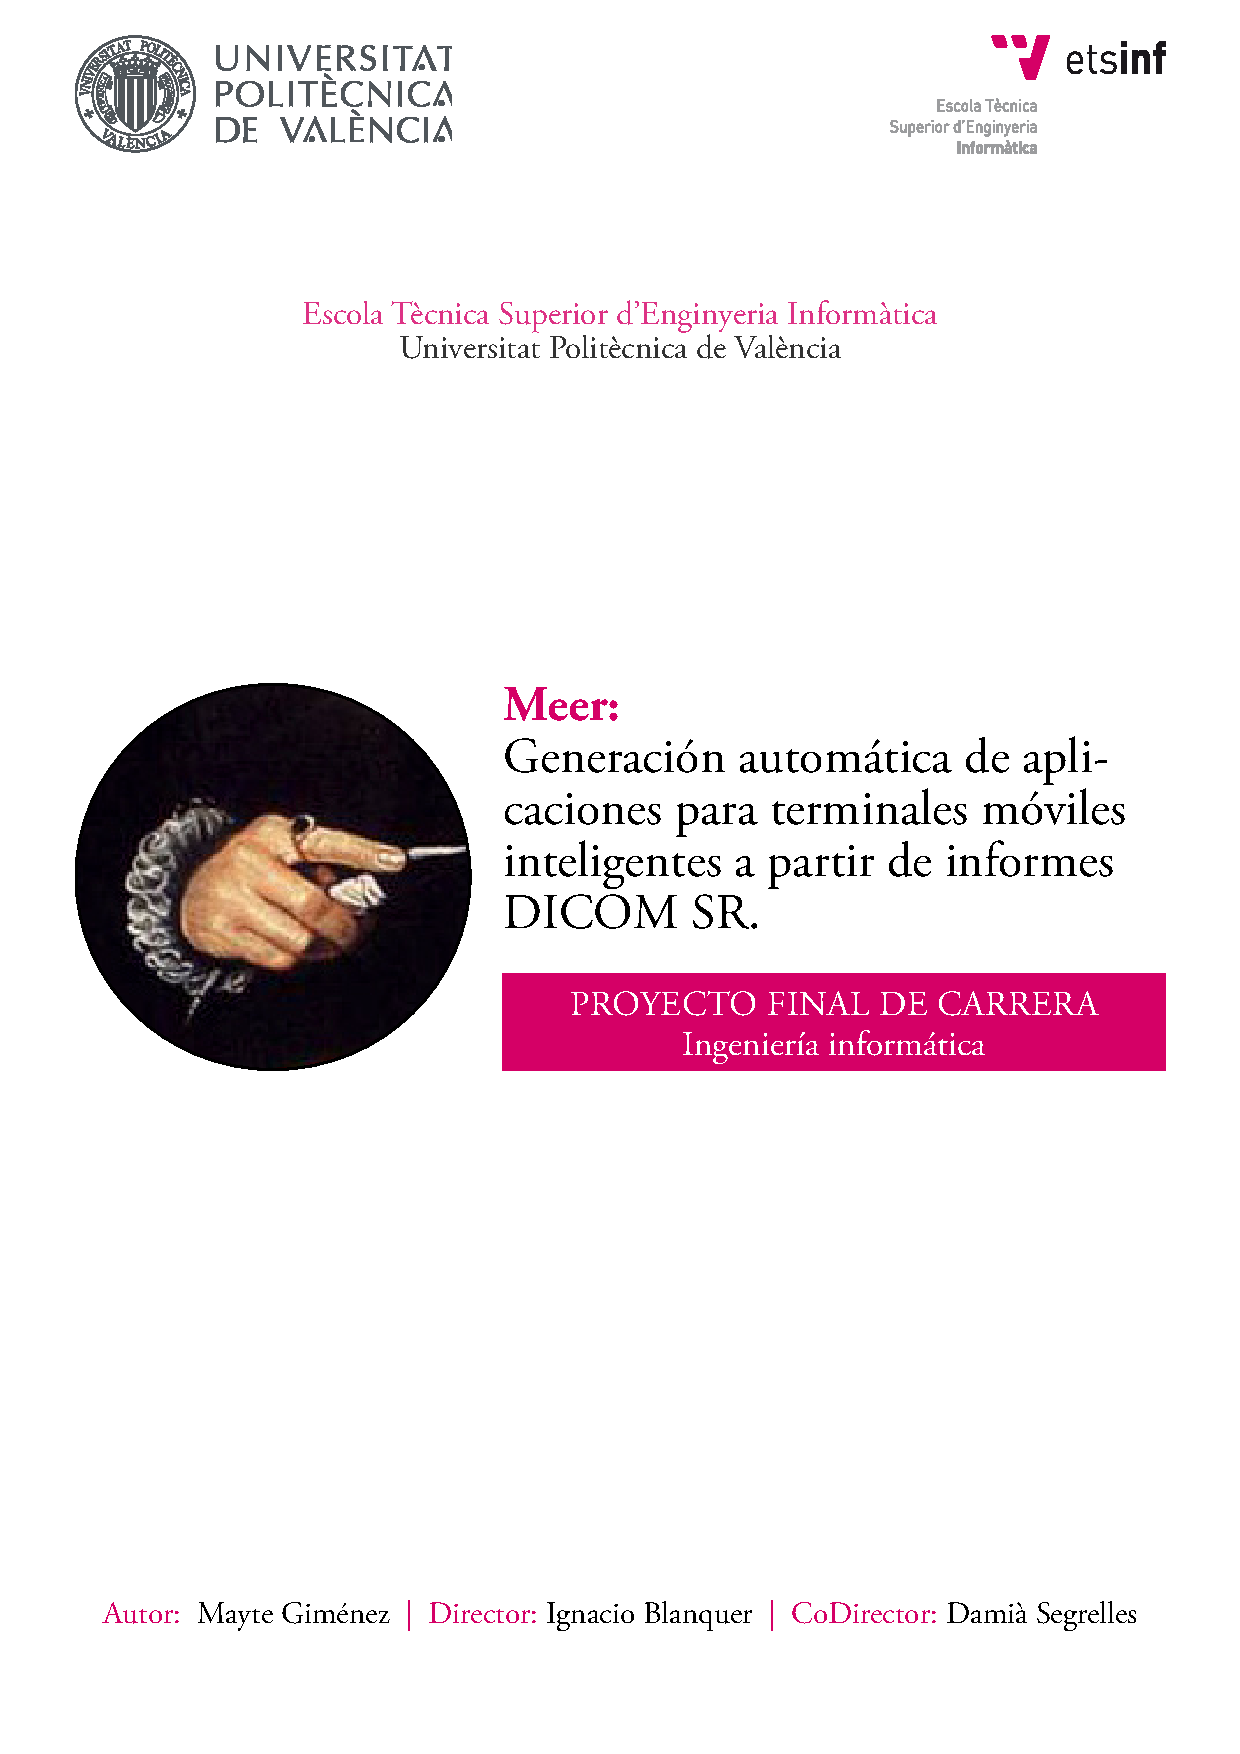
\includepdf[pages={1}]{./imgs/portada.pdf}

\begin{abstract}
El objetivo del siguiente Proyecto Fin de Carrera consiste en el desarrollo de una aplicación que a partir de un esquema de un informe médico, codificado en el estándar DICOM-SR, genere de manera automática una aplicación para dispositivos móviles de tipo Android de modo que facilite la adquisición de datos de pacientes e informes válidos.
\medskip  \par
El estándar Digital Imaging and Communication in Medicine (DICOM) define como tratar imágenes médicas desde su procesado hasta su comunicación. DICOM también especifica una extensión para soportar informes estructurados médicos (DICOM-SR), lo que ha permitido el desarrollo de distintas líneas de investigación basadas en este estándar. \medskip \par

En el ámbito médico, es fundamental que los datos adquiridos en los informes sean exhaustivos y fidedignos, sin embargo la gran versatilidad el estándar DICOM-SR hace que la propia adquisición de los datos sea un reto, en la que  la aparición y expansión de terminales móviles inteligentes pueden facilitar  la interacción entre el  usuario y la máquina. Estas tecnologías nos ofrecen la posibilidad de obtener datos de informes clínicos sin incrementar significativamente la carga de trabajo del personal médico. Por ello, son estas cualidades las que pretendemos explorar y explotar en este PFC, simplificando el proceso de adquisición de información para la obtención masiva de datos y de una mayor calidad.\par
Para ello se plantea como objetivo del PFC,  una aplicación para terminales Android, que permita al usuario introducir los datos de los informes estructurados basados en DICOMSR,  de un modo productivo, eficiente e intuitivo. La aplicación propuesta debe generar automáticamente a partir de un fichero plantilla donde se defina la estructura de informe DICOM-SR,  el código de la aplicación Android que proporcione la funcionalidad de inserción de informes.\par

\Keywords{DicomSR, Android, Python, Generación automática de código, imagen médica.}
\end{abstract}

\tableofcontents
\newpage

\listoffigures
\renewcommand\lstlistlistingname{Índice de código fuente}
\lstlistoflistings
\listoftables

\chapter{Introducción}
\section{Descripción del problema}\label{intro}
% Historia de los CADS y la imagen médica
Antes de profundizar en la descripción del problema que abordaremos en este proyecto final de carrera (PFC), hablaremos acerca del contexto en el que se inscribe.\medskip\par

La introducción de la imagen médica digitalizada ha transformado la práctica clínica. 
En la década de los 60 \cite{journals/cmig/Doi07} comienzan los esfuerzos por desarrollar líneas de investigación para el diagnóstico asistido por ordenador (CAD), pero no es hasta la década de los 80 cuando la tecnología permite que esta disciplina despegue. Solo como apunte para mostrar el impacto que tiene  el desarrollo de la imagen médica: la detección de cáncer de mama ha incrementado aproximadamente en un 10\% \cite{journals/cmig/Nishikawa07}, aunque podemos encontrar muchos otros ejemplos \cite{johnston1994effects, doi:10.1117/12.877968, kundel1975interpreting, Fujita:2008:CDE:1456710.1456735}.\medskip\par

% Historia de los PACs y DICOM
El formato de estas imágenes es crucial para el desarrollo de la investigación. Los Sistemas de Adquisición y Procesado de Imagen médica (PACs) \cite{huang2010pacs} contienen tanto el software como el hardware necesario para el tratamiento de la imagen médica.  Los principales elementos que forman los PACs son \cite{pianykh2012digital}:
\begin{itemize}
	\item \textit{Dispositivos de adquisición}: permiten la captura de la imagen médica. Estos dispositivos no tiene que compartir la misma tecnología de captura. Por lo que encontramos dispositivos de adquisición de imágenes como:
	\begin{itemize}
		\item Ultrasonidos.
		\item Resonancia magnética.
		\item Tomografía Axial Computarizada (TAC).
		\item Rayos X.
		\item \ldots
	\end{itemize}
	\item \textit{Archivos de la imagen médica}: servidores donde almacenar las imágenes.
	\item \textit{Estaciones de trabajo}: estaciones dónde los profesionales leen y trabajan con estas imágenes. 
\end{itemize}

 En la figura \ref{fig:pacs} vemos un esquema de los sistemas de adquisición y procesamiento de la imagen médica que acabamos de describir.\par
\begin{figure}[ht]
\centering
\includegraphics[scale=0.6]{./imgs/esquemas/pacs.pdf}
\caption{Componentes principales de los PACs}
\label{fig:pacs}
\end{figure}

\medskip\par

Y aunque en los inicios de estos sistemas cada fabricante comenzó desarrollando su propio formato para el majejo de las imagenes \cite{huang2011short, lemke2011short}, no tardaron en aflorar problemas derivados de la falta de un estándar para compartir y estudiar estas. Por este motivo surge en 1983 el estándar  Digital Imaging and Communication in Medicine (DICOM).\medskip\par

DICOM es un estándar \cite{bidgood1992introduction} desarrollado por el colegio Estadounidense de Radiología (ACR) y la asociación Nacional de Fabricantes eléctricos (NEMA), especifica no  solo el formato de las imágenes sino también como deben ser almacenadas, los protocolos para el intercambio de las mismas. \par
En los veinte años de vida el estándar no ha dejado de crecer. Se han desarrollado más de 160 suplementos al mismo que completan las carencias detectadas en su uso y se adaptan a las nuevas tecnologías. Entre el 2006 y el 2013, los temas en los que se ha centrado el foco de atención son la mejora en las tecnologías para la adquisición de las imágenes y los informes estructurados asociados a estas.\cite{dicomtrends}.
Precisamente de estos dos temas dan pie a dos líneas de investigación bien diferenciados en la literatura \cite{torres2012improving}:
\begin{itemize}
	\item \textit{Imagen médica}: cómo almacenar y procesar la información de las imágenes médicas. 
	\item \textit{Informes médicos}: informes estructurados con información de las imágenes.  
\end{itemize}
\medskip\par

Es precisamente en esta segunda rama de la investigación en la que nos centraremos en este PFC. Concretamente dentro del estándar DICOM, se especifica una extensión para tratar con los informes médicos estructurados, se trata del estándar DICOM-SR \cite{clunie2000dicom}, del cual relegamos una definición más en profundidad en el aparatado \ref{dicomSR}.\par
La correcta estructuración de los informes permite organizar el conocimiento sobre las imágenes, permitiendo comparar imágenes de manera precisa mediante métodos cuantificables, y con esta información mejorar el diagnóstico.  Estos informes estructurados, (así como la imagen médica) ofrece a los profesionales sanitarios herramientas de apoyo a la medicina basada en evidencias \cite{Sackett19973, Darlenski2010553, Elphick2004525}, y con los datos necesarios para entrenar a los sistemas de diagnostico asistidos por ordenador.\medskip\par

En la literatura podemos encontrar diferentes esfuerzos por mejorar el tratamiento del conocimiento contenido en los informes médicos\cite{BlanquerEspert:2009:COV:1528937.1529213,journals/jbi/TorresQEH12, journals/jamia/Tirado-RamosHL02}  y de la utilidad del uso de los informes DICOM-SR. \par
Pero lo que es evidente es que para que los estudios derivados de los informes médicos estructurados (DICOM-SR) sean eficaces necesitamos disponer de un conjunto amplio y preciso de estos. Aunque el uso de métodos estadísticos nos ayuda a paliar en  este problema, los modelos que se generen a partir de los datos y por extensión las conclusiones a las que pudiéramos llegar, serían en el mejor de los casos imprecisos. \par
Paradójicamente, nos encontramos con un cuello de botella en la adquisición de los datos en los informes DICOM-SR a partir de la imagen médica, ya que este proceso debe hacerlo un profesional. Rellenar formularios electrónicos pude ser una tarea tediosa, por lo que en la actualidad se emplea el reconocimiento del habla  para transcribir los informes de los profesionales como texto plano. Pero el lenguaje natural es impreciso por lo que se necesitan herramientas para aplicar la estructura de un informe DICOM a este texto plano \cite{sevenster2012aut, 9227155, citeulike:191295}. \medskip\par

Y es en este punto dónde encontramos el problema que queremos abordar. Necesitamos informes médicos estructurados, pero su adquisición es demasiado costosa y poco productiva de la manera tradicional, ya que la interacción requerida para que el usuario introduzca los datos es poco intuitiva y monótona, y las herramientas para aplicar la estructura del informe médico DICOM-SR al texto plano se ciñen a tipos de imagen concretos (Radiografías, radiologías,\ldots) debido a la complejidad de interpretar correctamente el lenguaje natural.\medskip\par

El otro elemento que nos hace falta para terminar de definir el problema, nos vincula con la solución que propondremos en el apartado \ref{solucion}, y es que afortunadamente las nuevas tecnologías nos ofrecen nuevas posibilidades. La interacción con los terminales móviles inteligentes han demostrado ser mucho más intuitiva y amigable para todo tipo de usuarios.\par
En los últimos años podemos encontrar trabajos que han comenzado a introducir terminales móviles inteligentes en el campo médico con resultados satisfactorios. \cite{journals/jdi/ChoudhriR11,20359897,journals/jdi/TangLLC04}\bigskip\par

Recapitulando, la existencia de estándares en la imagen médica ha facilitado el desarrollo de distintas líneas de investigación que han revolucionado la práctica clínica. \par
Los informes estructurados son una valiosa fuente de información médica, pero su adquisición requiere aumentar la carga de trabajo de los profesionales. \par
Los terminales móviles ofrecen nuevas formas de interactuar con los usuarios de manera más intuitiva, y su uso en el ámbito médico se ha probado productivo. \par


\section{Solución propuesta}\label{solucion}
La solución que se propone para el problema que hemos descrito en el apartado anterior, explota las ventajas que nos ofrecen los terminales móviles. Lo que se propone es desarrollar una aplicación que permita generar automáticamente una aplicación para terminales móviles inteligentes con el sistema operativo Android a partir de plantillas de los informes médicos estructurados (DICOM-SR).\medskip\par

Partimos de ficheros que sigan el estándar para informes médico DICOM-SR con la definición de la plantilla del tipo de informe en el que estamos interesados. Estos ficheros contienen información  acerca del tipo de informe, así como de todos los campos que deben estar presentes en el mismo; también contiene para cada campo información acerca del tipo, de las propiedades de cardinalidad, verificación de los mismos y posibles valores a asignar.\par

A partir de estos ficheros, extraeremos la información de los mismos y generamos el código necesario para crear un aplicación para terminales móviles inteligentes Android. Una vez hemos generado todos los ficheros necesarios (interfaz, modelo de clases, interacciones entre la interfaz de usuario, \ldots), los integraremos en el esqueleto de una aplicación Android estándar para este propósito, y de este modo tendremos el informe estructurado, convertido en una aplicación para terminales inteligentes.\par
En la figura \ref{fig:basic_schema}, podemos ver un esquema muy básico de la solución propuesta: la entrada del sistema es el fichero con la plantilla DICOM-SR, que se pasa a la aplicación en python que hemos desarrollado y esta genera una aplicación en Android con los datos del informe estructurado DICOM-SR. Entraremos en más detalles acerca de la arquitectura y la justificación de los detalles técnicos de la solución en los siguientes apartados.\bigskip\par

\begin{figure}[ht]
\centering
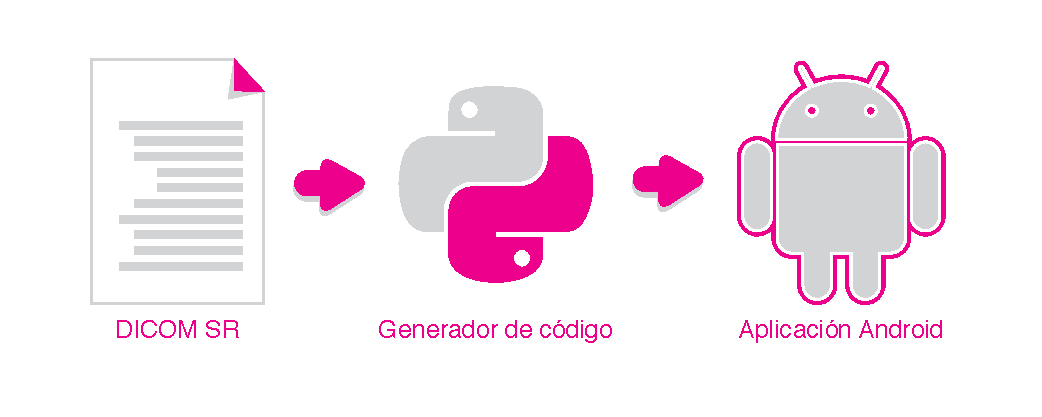
\includegraphics[scale=0.6]{./imgs/esquemas/simple.pdf}
\caption{Esquema básico}
\label{fig:basic_schema}
\end{figure}

El objetivo que pretendemos lograr con esta solución es claro: hacer uso de una interfaz de usuario muy intuitiva característica de los terminales móviles inteligentes, para interactuar con el usuario. Cuanto más podamos simplificar el trabajo del usuario a la hora de codificar los informes, más probablemente el profesional introduzca un número mayor de informes y de una forma más productiva. \medskip\par
La solución propuesta tiene varios puntos fuertes, que son los siguientes:
\begin{itemize}
\item Se trata de una solución \textit{genérica}. Independientemente del tipo de informe médico podemos de manera automática crear una aplicación Android que lo soporte.
\item Es \textit{adaptable} a los cambios en la plantilla DICOM-SR. Si añadimos nuevos campos, o modificamos el tipo de los mismos, la aplicación que se generaría cambiaría adaptándose a los cambios realizados en el informe.
\item Es \textit{configurarle}, ya el usuario podría decidir la configuración más intuitiva para él/ella.
\item La \textit{ubicuidad} de los terminales Android aporta al usuario la posibilidad al personal médico de comenzar la introcción de los datos en una pantalla táctil y continuar en una tableta. 
% TODO: Añadir la cita a los léxicos
\end{itemize}
\medskip\par

En definitiva, se trata de una solución que busca que los profesionales médicos introduzcan los datos de las imágenes que analicen en los informes médicos estructurados de tipo DICOM-SR  de una manera rápida e intuitiva. Los datos específicos de cada paciente introducidos por el profesional interactuando con la aplicación Android, se guardarán de nuevo en el formato estándar DICOM-SR. 

\chapter{Objetivos}

En este apartado enumeraremos los objetivos que se pretenden alcanzar por parte de la alumna durante el desarrollo de este proyecto final de carrera.\par
Esto nos permitirá acotar el alcance del proyecto y establecer los hitos a alcanzar, permitiendo elaborar una planificación lo más precisa posible.\medskip\par

Los objetivos a lograr son los siguientes:
\begin{itemize}
	\item Demostrar la habilidad para emprender un proyecto parcialmente autónomo a partir de lo estudiado durante el periodo de formación académica en la Ingeniería Informática.
	\item Comprender la estructura de los informes médicos de tipo DICOM-SR y ser capaz de interpretar su contenido.
	\item Desarrollar una aplicación que realice el análisis sintáctico y semántico de ficheros DICOM-SR.
	\item Desarrollar una aplicación Android genérica para generar interfaces que permitan la introducción de informes DICOM-SR en base a plantillas.
	\item Desarrollar una aplicación que a partir de un fichero DICOM-SR genere los ficheros necesarios para completar la aplicación Android básica para el informe concreto de entrada. 
	\begin{itemize}
		\item Comprender la generación de código haciendo uso de plantillas.
	\end{itemize}
	\item Realizar las pruebas pertinentes a la aplicación para un informe concreto. Estas pruebas las aplicaremos exhaustivamente a 4 ontologías:
	\begin{itemize}
		\item Exploración de mama.
		\item Mamografía.
		\item Ultrasonidos
		\item Resonancia magnética.
	\end{itemize}
	Y consistirán en realizar las siguientes tareas:
	\begin{itemize}
		\item Generar el código XML para soportar la internacionalización
		\item Generar el código XML que desarrolle la interfaz de usuario. 
		\item Generar el código XML con las propiedades de la aplicación Android.
		\item Generar el código java que codifique los modelos de clase del informe. 
		\item Generar el código java que codifique las interacciones entre actividades.
		\item Integrar todo el código generado dentro de la aplicación base de Android. 
		\item Comprobar su correcto funcionamiento en terminales físicos.
	\end{itemize}
\end{itemize}
\medskip\par
Aunque no sea estrictamente necesario, hemos creado un diagrama de Gantt que podemos ver en la figura \ref{fig:gantt}, que nos ayude a planificar el tiempo para lograr los objetivos que acabamos de describir.\par
\begin{figure}[ht]
\centering
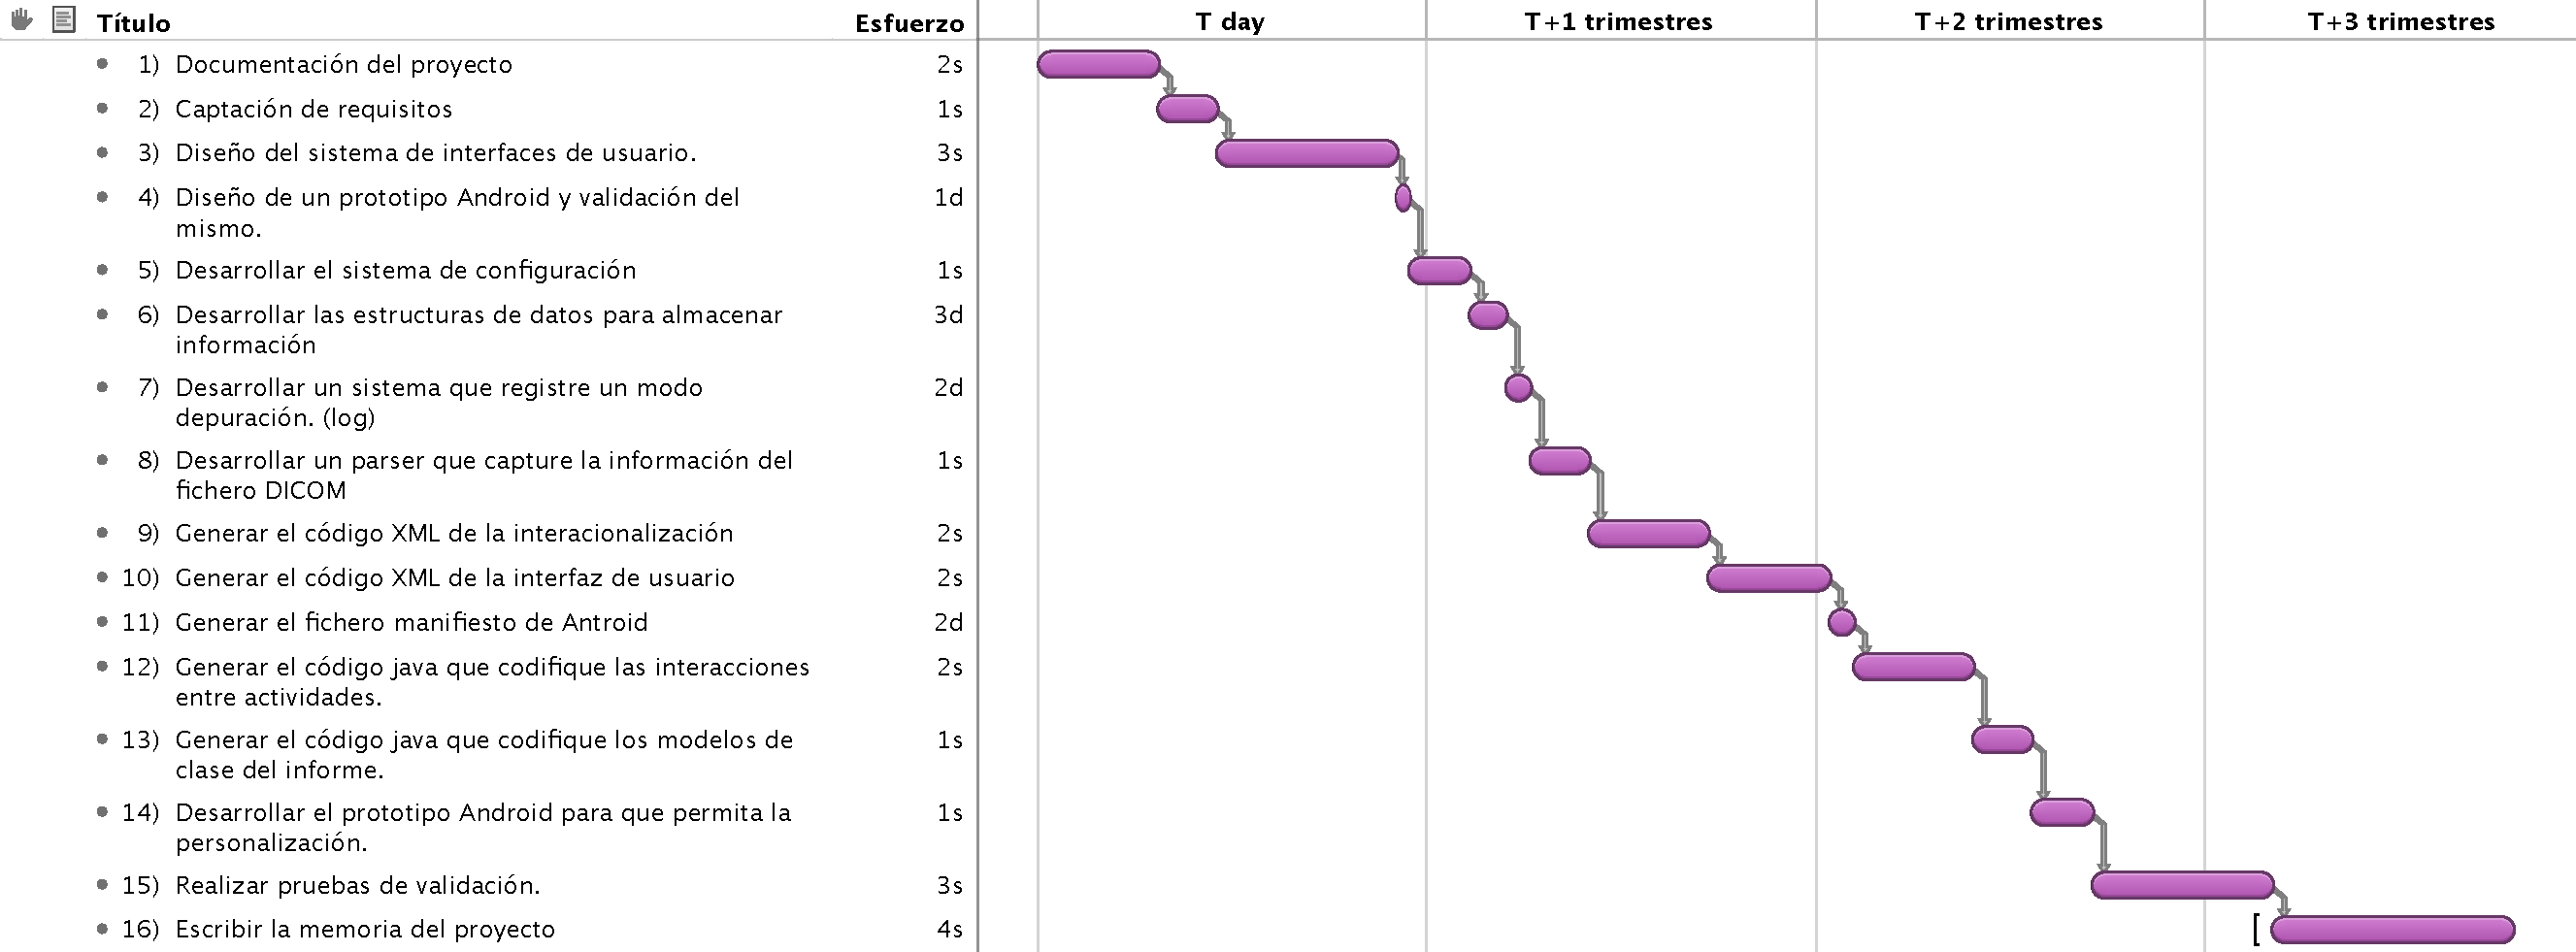
\includegraphics[scale=0.3]{./imgs/gantt.pdf}
\caption{Diagrama de Gantt}
\label{fig:gantt}
\end{figure}


\chapter{Estado del arte }\label{arte}
\chaptermark{Estado del arte}
Hasta este punto hemos introducido el problema y el contexto en el que ser circunscribe de manera generalista. En los siguientes apartados profundizaremos un poco más en el contexto del problema. Haremos un resumen del estado del arte de las áreas de conocimiento que vamos a trabajar. \medskip\par

\section{Imagen médica}
Situamos la primera imagen médica en 1895 con la imagen de rayos X de  Wilhelm Conrad Röntgen, pero no es hasta 1972 cuando encontraremos la primera imagen médica digitalizada: una tomografía computarizada de Godfrey Newbold Hounsfield. Paralelamente al desarrollo de la tecnología de los aparatos para la captación de imágenes hemos visto el desarrollo de las técnicas de la informática médica.\par
Encontramos en \cite{mantas2010recommendations}, una definición de lo que es la informática médica. Se trata del procesamientos sistemático de datos, información y conocimiento para la toma de decisiones óptima.\par
La medicina es un ámbito en que se puede aprovechar al máximo las nuevas posibilidades que nos ofrecen las tecnologías de la información. Es por esto que en los últimos 20 años hemos visto como ha florecido distintas líneas de investigación al rededor de la imagen médica.\par
Cuando hablamos de imagen médica nos referimos a un conjunto de técnicas y procesos para capturar imágenes del totales o parciales del cuerpo humano con propósitos cínicos.\cite{wiki:imgmedica}\par

En la literatura \cite{Muller20041,Maintz19981} podemos encontrar un repaso de los distintos dispositivos y tecnologías para captar imagen médica. Lo que es innegable es el gran impacto de la imagen médica en la práctica clínica. \medskip \par

Como afirmábamos en el apartado \ref{intro}, para hacer posible esta evolución son necesarios los estándares que permitan manipular las imágenes de manera óptima. Es precisamente por esto que se desarrolló el estándar de imagen médica DICOM. 
El acrónimo DICOM significa \textit{Imagen Digital y Comunicación en Medicina}. Por lo tanto no se trata únicamente del formato de la imagen sino que se diseñó para cubrir todas las necesidades vinculadas con la imagen médica. Necesidades como pueden ser: la compresión de imágenes, la comunicación, el almacenamiento, \ldots\par
Cada una de las necesidades específicas para el desarrollo de investigaciones y dispositivos relacionados con la imagen médica se recogen en el estándar y sus anexos que podemos encontrar en la web de la asociación Nacional de Fabricantes eléctricos (NEMA).\cite{nema}.\medskip\par

La literatura al respecto de la imagen médica en muy profusa. Por lo tanto, lo visto hasta el momento son únicamente los conceptos más básicos así como sus definiciones. La teoría sobre la imagen médica que hemos descrito forma parte de los cimientos sobre los que se sustenta este proyecto.\par

\section{Generación automática de código}\label{sec:generacion-codigo}
Otro de los pilares teóricos en los que se sustenta este proyecto es en la generación automática de código.\par
Cada una de las pruebas de imagen médica tiene asociado un informe DICOM-SR. Si nos planteáramos seguir un paradigma de programación diferente, necesitaríamos crear una aplicación Android para cada informe DICOM-SR. Aunque gran parte de este código fuera reutilizable, estaríamos desplazando el cuello de botella que ahora se encuentra en la captación de datos al desarrollo de aplicaciones.\par
Es por este motivo que optamos por la generación de código o traducción automática. Términos sinónimos en la literatura.\cite{802346}\medskip\par 
La generación automática de código es uno de los paradigmas de programación existentes y consiste en escribir programas que sean capaces de escribir el código fuente de otros programas basándose en modelos ontológicos.\par 
En nuestro caso los modelos ontológicos son las plantillas DICOM-SR. Para conseguir llevar a cabo esta tarea se dispone de un sistema de patrones que se instancian con los datos concretos, siguiendo unas reglas que son generalmente sencillas.\medskip\par
La generación automática de código es una de las líneas de investigación que más interés despierta en el ámbito de la ingeniería de software \cite{hinchey2005requirements}. Existe un buen número de razones para que esto sea así, a pesar de los desafíos que plantea este paradigma de programación. Entre los beneficios que ofrece la generación automática de código podemos enumerar los siguientes \cite{herrington2003code}:
\begin{itemize}
	\item \textit{Calidad}: El código generado mediante plantillas permite que la calidad sea consistente a lo largo de todo 	el software desarrollado y simplifica el proceso de aplicar parches que solucionen bugs. 
	\item \textit{Consistencia}: El estilo de programación mantiene una consistencia a lo largo de todo el software desarrolladoo.
	\item \textit{Más tiempo para el diseño del software y la arquitectura}: el análisis y desarrollo de la API en este paradigma es muy importante, por lo que se dedica más tiempo y recursos a captar los requisitos y crear la arquitectura. Estamos aprovechando el tiempo que de otro modo hubiéramos empleado en escribir manualmente el software.
	\item \textit{Abstracción}: la generación automática de código es independiente del lenguaje de programación, simplemente modificando el lenguaje de las plantillas podremos generar software en el lenguaje de programación que sea más conveniente. 
\end{itemize}
\medskip\par

La investigación actual tiene como gran reto el desarrollar modelos independientes del lenguaje y demostrar que el código que generan es computacionalmente equivalente al código generado por un desarrollador.\par
Sin embargo este enfoque queda fuera del alcance de nuestro proyecto. Lo que haremos es emplear las bases teóricas del paradigma de generación automática en nuestro desarrollo.\medskip\par
Existen diversas técnicas para generar código. Para este proyecto optamos por \textbf{generación parcial de clases}. La generación parcial de clases consiste en leer un fichero de texto con la información abstracta de las clases a generar, a continuación lee una serie de plantillas y con la información recogida de estas dos fuentes, generará el código necesario. Este código que hemos generado se integrará con el código escrito por ingenieros para formar la solución final.\par

En la figura \ref{fig:generacion} vemos como se aplica esta técnica de generación de código en nuestro ejemplo concreto. El sistema tendrá como entrada el informe médico de tipo DICOM-SR y una serie de plantillas, con esto generará el código necesario para que cuando lo integremos en la aplicación Android obtengamos una aplicación Android funcional específica para el informe de entrada. \par
\begin{figure}[ht]
\centering
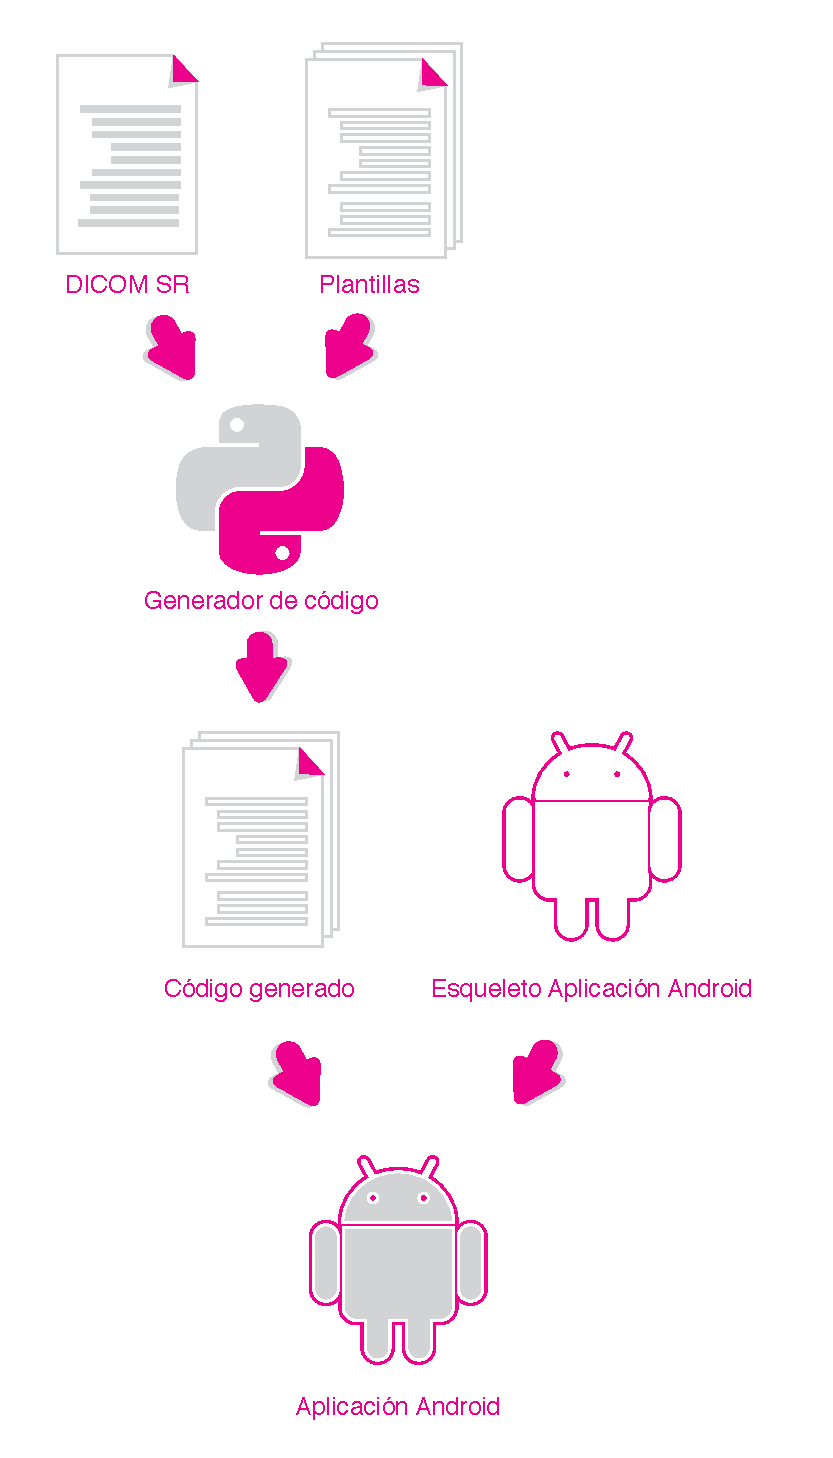
\includegraphics[scale=0.5]{./imgs/esquemas/generacion.pdf}
\caption{Generación parcial de clases}
\label{fig:generacion}
\end{figure}

\subsection{Desarrollo de software guiado por modelos}
El desarrollo de software guiado por modelos forma parte del paradigma de programación automática. De los paradigmas que descienden de la programación automática este es el que más se ajusta al trabajo que estamos presentando.\par
Consiste en desarrollar uno o varios modelos que representen el sistema y a partir de estos modelos se generará el software. Existen numerosas herramientas para definir modelos.\par
Según la literatura \cite{MDA} lo fundamental es que los modelos tengan las siguientes características:
\begin{itemize}
	\item Tan simples como sea posible (KISS).
	\item Canónico (DRY).
	\item Correcto nivel de abstracción.
	\item Separación de aspectos ( SoC ).
	\item Mantener modelos organizados y manejables.
	\item Independiente de la tecnología.
	\item Pragmáticos: sólo modelamos aquello que vayamos a emplear.
\end{itemize}
Podemos modelar todo o parte del sistema. Lo recomendable es que se modele aquello que varíe poco, con lo que el tiempo invertido en el modelado sea eficiente.\medskip \par

En nuestro caso el modelo viene determinado por el estándar soportado por los dispositivos PACs, es decir, utilizaremos los ficheros DICOM-SR como modelo para generar la aplicación.\par
Debido a las características del modelo, este proyecto no se adscribe dentro del desarrollo guiado por modelos tal y como se define en la literatura \cite{mdd}, pero si obviamos las características del modelo que vienen impuestas por los estándares médicos, seguimos la filosofía de este paradigma de programación, ya que a partir del modelo del sistema, el informe médico DICOM-SR, generamos el software con las características que el modelo define.\par


\section{Interacción persona-máquina y usabilidadad}\label{sec:UI}
\chaptermark{Usabilidad}
Por último, antes de cerrar este capítulo nos falta hablar del tercer pilar que sustenta este proyecto: la interacción persona-máquina.\par
Como hemos discutido en la introducción \ref{intro}, uno de los problemas a los que nos enfrentamos a la hora de recoger informes médicos es que rellenar estos informes es una tarea pesada para los profesionales clínicos que deben invertir mucho tiempo en la captación de requisitos. La tecnología per se no soluciona este problema, sino que nos da herramientas para afrontarlo. Lo que es importante es que realicemos un diseño de las interfaces de usuario centrándonos en las necesidades de las personas que utilizarán las aplicaciones.\medskip\par
El término Interacción Persona-Máquina (\textit{\textbf{H}uman-\textbf{C}omputer \textbf{I}nteraction} en inglés) no se popularizó hasta la década de los 80, aunque podemos encontrar raíces similares en los estudios de ergonomía de principios del siglo XX \cite{dix2004human}. Pero es con el auge de la informática y diseño de sistemas cuando el estudio de la Interacción persona-máquina comienza a desarrollarse plenamente de manera autónoma. Con la aparición de los ordenadores personales todo el mundo se convirtió en un usuario potencial y era necesario encontrar formas de interactuar adecuadamente con este nuevo público. \par
La Interacción Persona-Máquina se encarga del diseño, implementación y validación de las interfaces de usuario. Es decir, se encarga de modelar cómo los usuarios se relacionan con las máquinas.\medskip\par
Al desarrollar un proyecto de este tipo corremos el peligro cuando estemos absortos en los detalles técnicos de olvidar la importancia del diseño. Un buen diseño debe centrarse en las personas, y tiene un tremendo impacto en las tareas que realizan a pesar de que el diseño será transparente para los usuarios.\par
En ámbitos que incluyan sistemas críticos como puede ser la medicina, los fallos en el diseño de las interacciones pueden tener un gran coste económico y personal. A pesar de que nuestro ámbito de aplicación no es crítico tenemos presente que la aceptación del sistema por parte de los usuarios es un punto clave para resolver el problema que nos planteamos en este proyecto.\medskip \par
Los puntos claves para conseguir un buen diseño de interfaces se basan en que todo el sistema sea consistente y en solicitar información al usuario final acerca de sus impresiones y sensaciones con el diseño.\par 
Respecto a la consistencia, esta es una ventaja propia de la generación automática de código ya que mientras seamos consistentes en el diseño de las plantillas la aplicación final tendrá una aspecto coherente.\par
Para conseguir la información acerca de la idoneidad del diseño, el procedimiento consiste en crear un diseño y evaluar la satisfacción por parte de los usuarios, con las respuestas que obtenemos de nuestro usuarios, que idealmente será un grupo diverso que represente a las personas que utilizarán la aplicación, cambiamos el diseño y solicitamos de nuevo una evaluación del diseño. Idealmente seguiríamos iterando en el diseño de este prototipo hasta llegar a un punto en el los usuarios estén satisfechos con el resultado. En la práctica se llega a una solución de compromiso entre el tiempo empleado en el diseño y la satisfacción de los usuarios.\par
En nuestro proyecto hemos integrado los ciclos de diseño y validación de la interfaces dentro del desarrollo de la aplicación. En la fases iniciales de diseño, creamos las interfaces que se fueron refinando durante el proceso, y empleamos la aplicación Android que nos serviría de esqueleto dónde integrar el código generado como prototipo para poder validar el diseño.\medskip \par
Finalizamos este apartado recalcando la importancia del diseño, muchas veces denostado, en la aceptación por parte de los usuarios de las soluciones software que les proponemos. 



\chapter{Tecnologías empleadas en el proyecto}
En el capítulo \ref{intro} hemos planteado el problema y una posible solución al mismo. El objetivo tanto del capítulo anterior como este es el de sentar las bases teóricas y tecnológicas de la solución que hemos propuesto.\par 
Si en el capítulo  \ref{arte} repasábamos el estado del arte y sentábamos las bases teóricas del proyecto, en este capítulo describiremos la tecnología de la que hacemos uso para ejecutar de solución que proponemos. Además justificaremos los motivos que nos han llevado a seleccionar esta tecnología y no otra.\par

\section{DICOM-SR}\label{dicomSR}
En primer lugar hablaremos de la tecnología que nos impone el proyecto. Los PACs utilizan la extensión del estándar DICOM para informes estructurados(DICOM-SR) y como nuestro objetivo es que la solución se integre en el ecosistema existente en los centros médicos deberemos emplear este estándar.\medskip\par

\subsection{Definición}
DICOM-SR se incluye dentro del suplemento 23 del estándar de imagen médica DICOM. Describe una arquitectura de documento que permite compartir, almacenar y transmitir información de informes médicos estructurados \cite{hussein2004dicom}.\par
Se diseñó con la intención de suplir la brecha entre la información contenida en las imágenes y la información que los profesionales médicos introducen en estos. Los ficheros DICOM-SR almacenan de forma no ambigua y jerárquica todos los conceptos que podemos encontrar en un informe médico tradicional y además pueden incluir referencias a:
\begin{itemize}
	\item Imágenes en formato DICOM. 
	\item Informes de estudios previos.
	\item Detalles de las imágenes.
\end{itemize}\par\medskip\par
El estándar define el modelo de la información y cómo debe gestionarse el documento, lo que permite personalizar muchos aspectos de la implementación final\cite{hussein2004dicom2}.\par
Sin embargo al tratarse de un estándar bastante complejo, han surgido soluciones bastante dispares, entre las que podemos encontrar:
\begin{itemize}
	\item Una implementación basada en la orientación objetos integrando el estándar DICOM-SR en la estructura de XML.\cite{tirado2002information}
	\item Una implementación extendiendo el modelo de objetos de documento XML (DOM).\cite{doi:10.1117}
	\item Una implementación en C y C++ del estándar. \cite{Riesmeier2001795}
\end{itemize}
\par
Desde la Asociación Nacional de Fabricantes eléctricos (NEMA), se están haciendo esfuerzos por unificar los criterios y seguir avanzando en la definición del estándar.\par
Para este proyecto se emplea una implementación en la que el informe se estructura en un XML. Expondremos los detalles de los ficheros DICOM-SR con los que trabajaremos en los apartados \ref{dicomsr:ficheros},\ref{dicomsr:plantillas}, \ref{dicomsr:vocabulario} y \ref{dicomsr:internacionalizacion}.\par

\subsection{Beneficios del estándar DICOM-SR}\label{dicom:beneficios}
A pesar de los problemas que surgen en la definición y en la implementación del estándar, los beneficios que aporta su desarrollo merecen el esfuerzo. Podemos encontrar un resumen exhaustivo de las ventajas de DICOM-SR en el siguiente artículo \cite{noumeir2006benefits}. Entre las mejoras que aporta a la práctica clínica más relevantes encontramos: 
\begin{itemize}
	\item Mejora la comunicación entre los profesionales, al utilizar un léxico estándar no hay lugar a traducciones o 	interpretaciones erróneas. 
	\item Los informes son más precisos y concisos. Los profesionales rellenan el informe utilizando los códigos adecuados sin 	las estructuras gramaticales que serían necesarias al redactar los informes de modo tradicional. 
	\item Se evitan los errores gramaticales y de transcripción.
	\item La interpretación de los informes es más sencilla y permite una interpretación asistida por ordenador. 
	\item Las imágenes DICOM y los informes DICOM-SR comparten la misma cabecera que contiene información acerca del paciente, 	lo que mejora el registro de información médica.
	\item El informe incluye medidas numéricas de las evidencias encontradas, que redundará en la precisión del informe.
	\item Permite ejecutar acciones automáticas sobre los informes permitiendo la minería de datos.
	\item Se enfatizan los contenidos. El informe en DICOM-SR no guarda información de cómo debe mostrarse al usuario, separa el contenido de la presentación de los datos.
	\item Permite la transformación a otros formatos. 
	\item Permite la integración con sistemas que reconozcan el habla. 
\end{itemize} 
Como podemos comprobar el desarrollo del estándar tiene un impacto beneficioso directamente sobre la práctica clínica, es por esto que en los últimos 5 años ha crecido el interés de la comunidad científica por explotar el estándar DICOM-SR.\par

\subsection{Estructura de un informe médico estructurado} \label{dicomsr:ficheros}
A continuación describiremos las características de un informe médico DICOM-SR representado siguiendo el formato XML.\par
En un fichero XML que contiene un informe médico DICOM-SR, la información se organiza mediante contenedores \textit{<CONTAINER>}. Los contenedores no almacenan la información, únicamente la estructuran. Los contenedores tienen hijos \textit{<CHILDS>}, y es dentro de los hijos dónde se almacena la información correspondiente a un informe concreto. Cada elemento de información se agrupa con las etiquetas con el tipo del valor que designan el tipo de elemento que se almacena en el campo. En nuestro PFC soportamos las siguientes, aunque existen otros muchos:
\begin{itemize} 
 	\item \textit{<DATE>}: almacena fechas.
 	\item \textit{<TEXT>}: almacena texto sin formato.
 	\item \textit{<NUM>}: almacena enteros o boleanos.
 	\item \textit{<CODE>}: almacena campos multievaluados.
 \end{itemize}
Dentro de las secciones definidas por estas etiquetas de tipo valor encontramos los datos del informe médico en pares de elementos clave-valor. Para designar la clave utilizamos la etiqueta \textit{<CONCEPT\_NAME>}, mientras que para referirnos al valor de este contenedor utilizamos la etiqueta \textit{<VALUE>}.
En el ejemplo de la figura \ref{dicom-report-tags} podemos ver como se codifica el identificador \textit{M001} de una lesión de tipo masa. Vemos un contenedor que abarca el concepto \textit{masa} y entre los hijos encontramos el identificador de la masa que es de tipo texto.\par
En el campo valor, \textit{<VALUE>}, podremos encontrar entre otros:
\begin{itemize}
	\item Texto plano.
	\item Valores numéricos con sus unidades.
	\item Fechas.
	\item Referencias a imágenes DICOM.
	\item \ldots
\end{itemize}\par

Un punto importante para alcanzar los objetivos descritos en \ref{dicom:beneficios}, es trabajar con un léxico limitado y bien conocido, por lo que se utilizan diccionarios de conceptos médicos para identificar cada concepto de los que puede aparecer en un informe.Cada concepto del informe se identifica por su \textit{CONCEPT\_NAME} que está formado por tres elementos:
\begin{itemize}
	\item \textit{CODE\_SCHEMA}: identifica el diccionario dónde se encuentra el término que estamos definiendo.
	\item \textit{CODE\_VALUE}: es el código al término médico definido.
	\item \textit{CODE\_MEANING}: contiene una descripción en texto plano del término para que sea legible por el usuario.
\end{itemize}
La combinación de \textit{CODE\_SCHEMA} y \textit{CODE\_VALUE} identifica de modo único un concepto dentro del informe.\par
De nuevo empleando el ejemplo \ref{dicom-report-tags}, vemos que el concepto \textit{masa} se encuentra en el diccionario \textit{RADLEX} con el código \textit{RID3874}.\medskip\par

\lstset{escapechar=@,style=dicom}
\renewcommand*\lstlistingname{Código}
\begin{lstlisting}[label=dicom-report-tags,caption=Fragmento de un informe estructurado de una exploración de mama]
		  ...
          <CONTAINER>
            <CONCEPT_NAME>
              <CODE_VALUE>RID3874</CODE_VALUE>
              <CODE_SCHEMA>RADLEX</CODE_SCHEMA>
              <CODE_MEANING>Mass</CODE_MEANING>
            </CONCEPT_NAME>
            <CHILDS>
              <TEXT>
                <CONCEPT_NAME>
                  <CODE_VALUE>118522005</CODE_VALUE>
                  <CODE_SCHEMA>SNOMED-CT</CODE_SCHEMA>
                  <CODE_MEANING>Identifier</CODE_MEANING>
                </CONCEPT_NAME>
                <VALUE> M001 </VALUE>
              </TEXT>
              ...
\end{lstlisting}

La información DICOM-SR del informe rellena el árbol XML. Existen implementaciones del estándar que hacen uso de etiquetas específicas para indicar las relaciones entre los contenedores DICOM, pero debido a que los ficheros XML almacenan la información per se en forma de árbol estas etiquetas son redundantes.\par
En la figura \ref{fig:dicom-report} se puede ver un esquema del árbol de conceptos de un informe siguiendo el formato DICOM-SR. Se trata de un exploración de mama, en la que se ha encontrado una masa en la mama derecha y dos asimetrías en la mama izquierda. Los campos de tipo valor, es decir los atributos del contenedor padre los representamos utilizando los cuadrados grises. Mientras que los contenedores, que no almacenan información pero estructuran el informe, los representamos con los cuadrados magentas.\par
Podemos encontrar el fichero DICOM-SR completo del informe que representa esta figura en el apéndice \ref{dicom-sr}.	\par

\begin{figure}[ht]
\centering
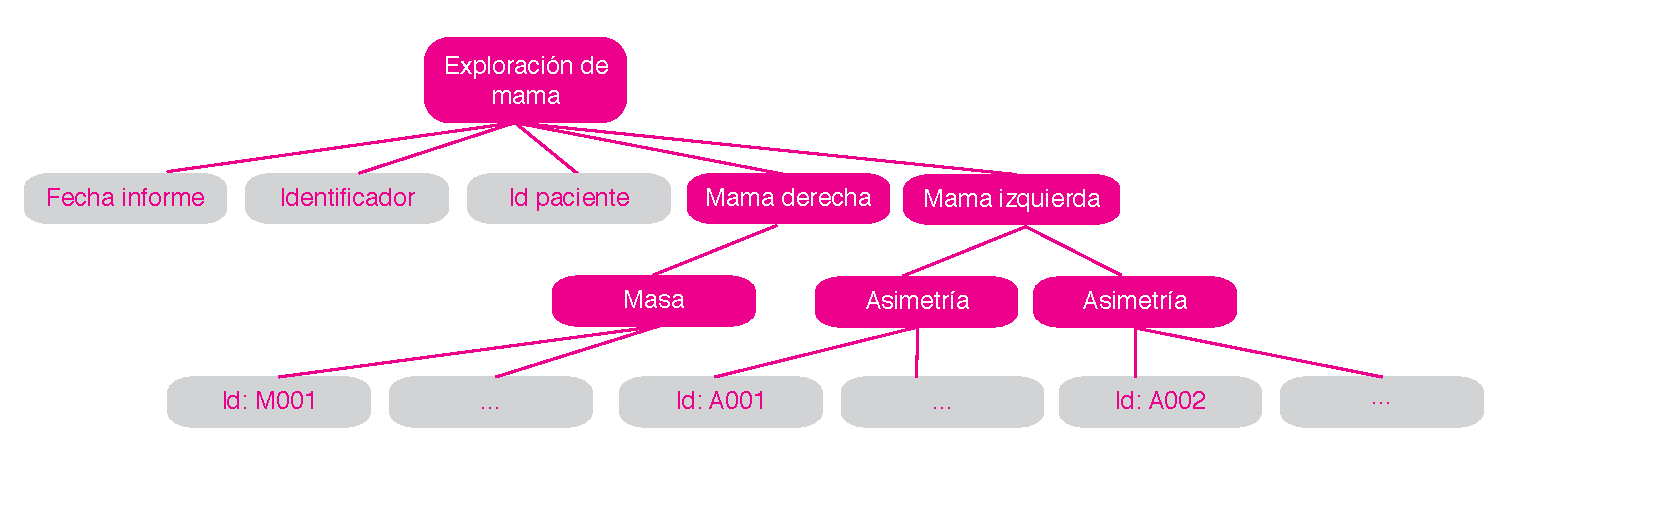
\includegraphics[scale=0.7]{./imgs/esquemas/dicomsrTreeReportA.pdf}
\caption{Representación del árbol XML de un informe en formato DICOM-SR}
\label{fig:dicom-report}
\end{figure}

\subsection{Estructura de una plantilla para un informe médico estructurado}\label{dicomsr:plantillas}
El estándar DICOM-SR, permite gran flexibilidad a la hora de escribir los informes estructurados. Esta característica puede complicarnos mucho el trabajo si cada especialista médico escribiera los informes siguiendo criterios correctos según el estándar pero aleatorios.
Para solucionar esto se crean las plantillas.
Las plantillas describen cómo debe ser un informe de tipo DICOM-SR, incluye los conceptos que debe tener así como las relaciones de jerarquía entre ellos y las propiedades que deben cumplir: si los conceptos son obligatorios o no, si pueden repetirse a lo largo del informe, \ldots\par 
Únicamente se guardan los conceptos en las plantillas, los campos correspondientes a los valores  \textit{<VALUE>} se incluirán después cuando el profesional rellene los datos para un paciente concreto.\par
El formato de las plantillas DICOM-SR es muy similar al de los informes DICOM. Carecen de las etiquetas \textit{<VALUE>} pero incluyen etiquetas \emph{<PROPERTIES>} para especificar las propiedades que deben tener los campos.\par
En el ejemplo de código \ref{dicom-template-mass} vemos como se almacenaría un concepto de tipo masa en una plantilla para la exploración de mama. Este contenedor podrá aparecer 0 o más veces en el informe final  (\textit{<CARDINALITY max=``-1'' min=``0''/>}) y lo introduce el usuario (\textit{<CONDITION\_TYPE type=``U''/>}).\medskip\par


\lstset{escapechar=@,style=dicom}
\renewcommand*\lstlistingname{Código}
\begin{lstlisting}[label=dicom-template-mass,caption=Fragmento de un plantilla informe estructurado: codificar una anomalía de tipo masa en una exploración de mama.]
		  ...
            <CONCEPT_NAME>
              <CODE_VALUE>RID3874</CODE_VALUE>
              <CODE_SCHEMA>RADLEX</CODE_SCHEMA>
              <CODE_MEANING>Mass</CODE_MEANING>
            </CONCEPT_NAME>
            <PROPERTIES>
              <CARDINALITY max="-1" min="0"/>
              <CONDITION_TYPE type="U"/>
              <EXPRESION_CONDITION xquery=""/>
            </PROPERTIES>
          ...
\end{lstlisting}

Además, en las plantillas de los contenedores se pueden incluir etiquetas para indicar la unidad de medida de los mismos, dentro de las etiquetas \emph{<UNIT\_MEASUREMENT>}. Estas etiquetas también servirán como modificadores como es el caso del ejemplo \ref{dicom-template-bool}, donde la etiqueta para el tipo del valor número, \textit{<NUM>}, se modifica de modo que el valor que introduzca el usuario será de tipo boleano, es decir sólo se permiten los valores 0 y 1. Así el concepto ``Cuadrante superior exterior de la mama derecha'' tendrá el valor verdadero o falso si la anomalía se sitúa en esa posición de la mama.\medskip\par

\lstset{escapechar=@,style=dicom}
\renewcommand*\lstlistingname{Código}
\begin{lstlisting}[label=dicom-template-bool,caption=Fragmento de una plantilla de un informe estructurado: codificar un atributo de tipo booleano.]
		  ...
              <NUM>
                <CONCEPT_NAME>
                  <CODE_VALUE>RID29929</CODE_VALUE>
                  <CODE_SCHEMA>RADLEX</CODE_SCHEMA>
                  <CODE_MEANING>Upper Outer Quadrant of Right Female Breast</CODE_MEANING>
                </CONCEPT_NAME>
                <PROPERTIES>
                  <CARDINALITY max="1" min="1"/>
                  <CONDITION_TYPE type="M"/>
                  <EXPRESION_CONDITION xquery=""/>
                  <DEFAULT_VALUE value="0"/>
                  <UNIT_MEASUREMENT>
                    <CONCEPT_NAME>
                      <CODE_VALUE>000000001</CODE_VALUE>
                      <CODE_SCHEMA>UNIT_MEASUREMENT</CODE_SCHEMA>
                      <CODE_MEANING>Boolean Units</CODE_MEANING>
                    </CONCEPT_NAME>
                  </UNIT_MEASUREMENT>
                </PROPERTIES>
              </NUM>
              ...
\end{lstlisting}

Las plantillas deben sintetizar el conocimiento de los especialistas técnicos que conozcan el estándar DICOM-SR y los profesionales médicos que conocen las características que deben tener los informes de las pruebas clínicas, por lo que será imprescindible la colaboración entre los profesionales de ambos ámbitos para crear las plantillas DICOM-SR.\medskip\par

Utilizamos estas plantillas como entrada para nuestro sistema. Tenemos una plantilla por ontología de exploración médica. Para este proyecto estamos trabajando con 4 ontologías diferentes.
\begin{itemize}
	\item Exploración de mama.
	\item Mamografía.
	\item Escáner de ultrasonidos.
	\item Resonancia Magnética
\end{itemize}

En el caso de las plantillas la información también se estructura en forma de árbol. En el apéndice \ref{dicom-sr-template}, hemos incluido una plantilla truncada para el informe de una exploración de mama. En este apéndice se describe una plantilla que permite introducir lesiones de tipo masa en la mama derecha y asimetrías en la mama izquierda. El esquema \ref{fig:dicom-template} muestra esta plantilla con su  forma arbórea.\medskip\par

\begin{figure}[ht]
\centering
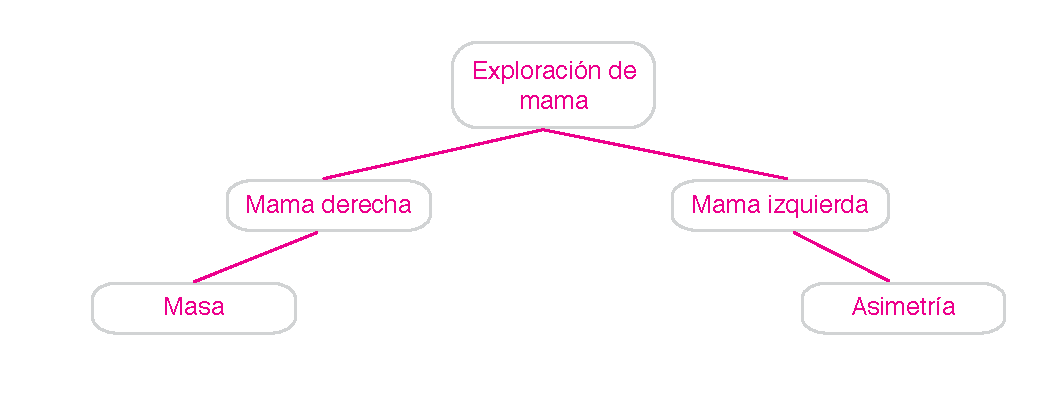
\includegraphics[scale=0.7]{./imgs/esquemas/dicomTreeTemplate.pdf}
\caption{Representación del árbol XML de una plantilla para un informe en formato DICOM-SR}
\label{fig:dicom-template}
\end{figure}


\subsection{Vocabulario}\label{dicomsr:vocabulario}
Un punto en el que hemos hecho hincapié es en la ventaja que supone que los informes hagan uso de un vocabulario estandarizado. Esto permite hacer referencia a conceptos concretos de manera precisa. Evitando los problemas que supone la barrera lingüística y la falta precisión del lenguaje natural.\medskip\par
También en lo que respecta al uso de vocabularios médicos DICOM-SR permite gran flexibilidad, permitiendo a los usuarios seleccionar el léxico que más les convenga en cada momento. En un mismo informe estructurado DICOM-SR pueden aparecer varios vocabularios.\par
Los vocabularios más habituales que podemos encontrar son: 
\begin{itemize}
	\item \emph{RadLex}: léxico desarrollado para cubrir las necesidades de la imagen radiológica. Contiene más de 30.000 términos \cite{langlotz2006radlex}.
	\item \emph{ICD-10}: léxico generalista que contiene un índice internacional de enfermedades y problemas relacionados con la salud. Está traducido en 42 idiomas \cite{world2004icd}.
	\item \emph{SNOMED-CT}: se considera la terminología clínica que más términos abarca y que soporta más lenguajes \cite{stearns2001snomed}. Se está convirtiendo en un estándar de facto al estar apoyado por numerosos gobiernos internacionales \cite{snomed-gov}.
\end{itemize}
\medskip\par
Sin embargo estos léxicos también presentan algunos inconvenientes: los conceptos pueden aparecer en varios léxicos, existen léxicos muy específicos para un país o idioma\ldots\medskip\par
Para este proyecto utilizaremos los siguientes léxicos:
\begin{itemize}
 \item Estándares internacionales:
 \begin{itemize} 
  \item \emph{RadLex}. 
  \item \emph{SNOMED-CT}.
 \end{itemize}
 \item Vocabularios definidos por nostros:
 \begin{itemize} 
  \item \emph{TRENCADIS\_MAMO}.
  \item \emph{UNIT\_MEASUREMENT}.
 \end{itemize}
 \end{itemize}
  \par
	
\subsection{Internacionalización}\label{dicomsr:internacionalizacion}
Las máquinas pueden trabajar con códigos como los que se almacenan en los léxicos médicos, incluso para algunas tareas puede ser incluso más beneficioso que tener que lidiar con secuencias de caracteres, especialmente si estos incluyen caracteres especiales. Pero las personas necesitamos el vocabulario para comprender los conceptos y poder trabajar con ellos.\medskip \par

La internacionalización y localización consiste precisamente en adaptar el software a los distintos idiomas y a las diferencias regionales como puedan ser los formatos de las divisas. No se trata únicamente de traducir las cadenas de texto.\par 
La internacionalización es la primera parte del proceso, consiste en diseñar y preparar el software que vamos a desarrollar y la localización es el proceso de adaptar el software creado a los distintos idiomas que se soporten \cite{Uren:1993:ISI:562752}. \medskip\par

Para presentar el informe a los profesionales médicos hacemos uso del texto codificado en las etiquetas \emph{<CODE\_MEANING>}. Sabiendo que algunos de los léxicos que se pueden incluir dentro un informe estructurado DICOM-SR están traducidos a múltiples idiomas, necesitamos encontrar una manera de que el significado del concepto sea diferente para cada lenguaje.\par
El estándar DICOM-SR especifica que las cadenas que se introduzcan en el campo \emph{<CODE\_MEANING>} pertenezcan al léxico con el que se esté trabajando, lo que no implica que estos textos deban estar en inglés, pero restringe la posibilidad de implementar soluciones en las que las traducciones no provengan de fuentes oficiales, porque esto nos conduciría de nuevo a la confusión semántica que pretendíamos evitar con el uso de vocabularios.\par
La solución que se propone en la literatura \cite{clunie2000dicom}, es hacer uso de la codificación del fichero para deducir el lenguaje del mismo, pero aunque se trata de una solución sencilla que no implica tener que trasmitir ni almacenar más información, si varios idiomas pueden utilizar la misma codificación no hay ninguna manera de diferenciarlos siguiendo este método. La otra solución que se propone es utilizar una etiqueta para identificar el idioma. Los ficheros XML con los que trabajamos optan por la segunda opción. Utilizan la etiqueta \emph{<CODE\_MEANING>} para un primer idioma y \emph{<CODE\_MEANING2>} para un segundo como podemos ver en el ejemplo \ref{code-meaning}.\par

\lstset{escapechar=@,style=dicom}
\renewcommand*\lstlistingname{Código}
\begin{lstlisting}[label=code-meaning,caption=Internacionación y localización en ficheros DICOM-SR.]
		  ...
  <CONTAINER>
    <CONCEPT_NAME>
      <CODE_VALUE>RID10312</CODE_VALUE>
      <CODE_SCHEMA>RADLEX</CODE_SCHEMA>
      <CODE_MEANING>Resonancia Magnética</CODE_MEANING>
      <CODE_MEANING2>Magnetic Resonance Imaging</CODE_MEANING2>
    </CONCEPT_NAME>
              ...
\end{lstlisting}


En nuestro PFC trabajaremos con plantillas localizadas para castellano e inglés como las que hemos visto en el ejemplo \ref{code-meaning}, así como con plantillas únicamente en inglés sin localizar como los fragmentos vistos en los ejemplos \ref{dicom-report-tags}, \ref{dicom-template-mass} y \ref{dicom-template-bool}

\section{Android}
Los teléfonos móviles inteligentes y las tabletas son tecnologías que ya llevan bastante tiempo entre nosotros, pero es en los últimos cinco años cuando la tecnología ha crecido exponencialmente. El índice de penetración en el mercado supera el 50\% en el caso de China y Estados Unidos, mientras que en Europa encontramos porcentajes inferiores, alrededor del 25\% pero las previsiones estiman que estas tasas crezcan rápidamente \cite{wiki:smartphones}.\par
La integración de dispositivos, la posibilidad de acceder a Internet y sobretodo la simplicidad de su uso fomentada por la posibilidad de interactuar con el dispositivo a través de la pantalla táctil, mucho más intuitivo que el teclado y el ratón, junto con un muy buen diseño de interfaces han facilitado la gran adopción de esta tecnología ya que han conseguido ampliar el espectro de usuarios potenciales\medskip\par

Un punto fundamental en el éxito de estas tecnologías es sin duda el nacimiento de Android.\par
Android es un sistema operativo basado en Linux, diseñado para trabajar con dispositivos móviles con pantallas táctiles. Fue desarrollado inicialmente por Android Inc., que fue comprada por Google en 2005. En el 2007 se forma la Open Handset Alliance: un conglomerado de empresas de hardware, software y telecomunicaciones cuyo objetivo es el de crear un entorno estandarizado para el desarrollo de dispositivos móviles. La OHA disponía de todos los agentes necesarios para revolucionar el mercado de las comunicaciones móviles y es en Octubre de 2008 cuando aparece el primer teléfono inteligente el HTC Dream que corría un Android 1.0. \cite{wiki:android}.\medskip\par

A partir de este momento el desarrollo de Android no ha dejado de crecer, convirtiéndose en una tecnología clave.\par
Como ya se ha comentado en el apartado \ref{intro}, el uso de terminales móviles inteligentes en la práctica clínica para trabajar con imagen médica ha dado resultados muy satisfactorios. Por lo tanto, es obvio pensar que una aplicación para recopilar informes médicos sobre Android tendrá mejor acogida por parte del personal médico, ya que es más sencillo e intuitivo introducir los datos de los informes DICOM-SR. Y al facilitar esta tarea al personal médico, es más factible que podamos adquirir más informes DICOM-SR con los que realizar estudios posteriores.\par 

\subsection{Arquitectura}
En este apartado hablaremos brevemente de la arquitectura de Android.\par
Android es un sistema operativo abierto basado en Linux, cuyo núcleo está escrito en C y C++, y que fundamentalmente tiene soporte para Java. Google libera periódicamente el código del sistema operativo bajo la licencia Apache.\par 
\begin{figure}[ht]
\centering
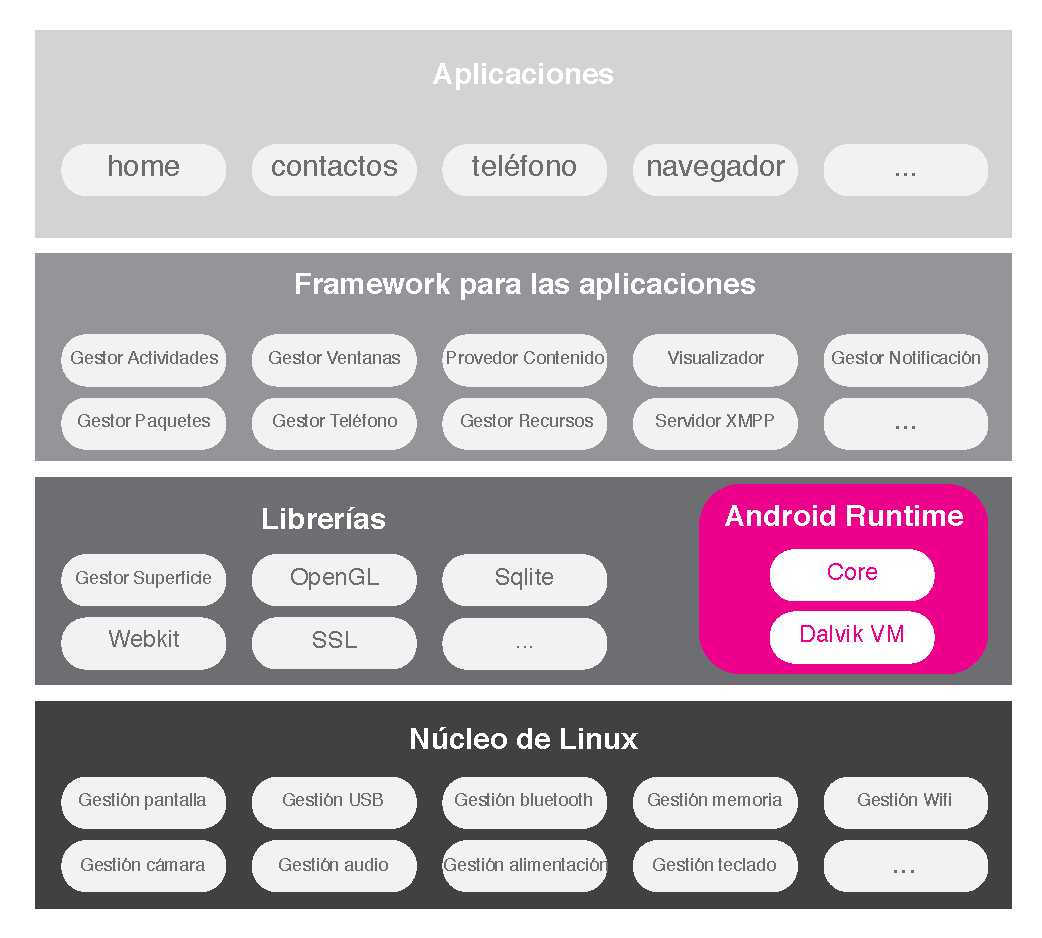
\includegraphics[scale=0.8]{./imgs/esquemas/arquitectura.pdf}
\caption{Arquitectura Android}
\label{fig:arquitectura_android}
\end{figure}

En la figura \ref{fig:arquitectura_android} vemos un esquema de la arquitectura Android, compuesta por:
\begin{itemize}
\item \emph{Núcleo Linux}: el núcleo es un fork de la versión 2.6 de Linux. Sirve de abstracción con el hardware y gestiona los recursos del sistema. 
\item \emph{Librerías}: librerías nativas del sistema las utilizará el framework de Android para comunicarse con el hardware. Están escritas en C o C++.
\item \emph{Android Runtime}: se trata del entorno de ejecución de Android. Se integra con las librerías. Aquí tenemos el conjunto de librerías habituales de java, así como librerías Java específicas para Android. La Dalvik VM, es la máquina virtual de Java que ejecutará la aplicaciones. 
\item \emph{Framework para aplicaciones}: Capa formada por las clases y servicios que utilizan directamente las aplicaciones de usuario para interactuar con Android. 
\item \emph{Aplicaciones}: esta última capa incluye todas las aplicaciones del sistema y las instaladas por el usuario, tanto las nativas como las escritas en java.

\end{itemize}




\subsection{Segmentación}
El hecho de que exista una amplia gama de dispositivos que utilizan Android como sistema operativo también tiene una parte negativa y es que los terminales más antiguos ejecutan versiones obsoletas de Android y no es posible actualizarlos. Lo que lleva a que en el mercado convivan distintas versiones de Android.\par

La segmentación es uno de los problemas con los que tiene que lidiar Android. En la actualidad conviven 7 distribuciones de Android.\par
Desde la web de Android \cite{android} mantienen una tabla con el porcentaje de dispositivos que usan cada versión (tabla \ref{android:distro}).\medskip\par

\begin{table}
\begin{center}

  
  \begin{tabular}{ |l|l|l|l| }
    \hline
    \rowcolor{RubineRed} {\color{White} Versión} & {\color{White} Nombre }& {\color{White} Nivel API }& {\color{White} Distribución} \\ \hline
    1.6 & Donut & 4 & 0.1\%  \\ \hline
    2.1 & Eclair & 7 & 1.2\%  \\ \hline
    2.2 & Froyo & 8 & 2.5\%  \\ \hline
    2.3-2.3.2 & Gingerbread & 9 & 0.1\%  \\ \hline
    2.3.3-2.3.7 & Gingerbread & 10 & 33.0\%  \\ \hline
    3.2 & Honeycomb & 13 & 0.1\%  \\ \hline
    3.2 & Ice Cream Sandwich & 15 & 22.5\%  \\ \hline
    4.1 & JellyBean & 16 & 34.0\%  \\ \hline
    4.2 & JellyBean & 17 & 6.5\%  \\ \hline
    
    \end{tabular}
\end{center}
\caption{Distribución de las versiones de la plataforma Android}
  \label{android:distro}
\end{table}

Lo que recomienda Google a la hora de seleccionar una versión de Android es que lleguemos a una solución de compromiso entre las características que necesitamos utilizar de la API y el porcentaje de dispositivos en los que nuestra aplicación se podrá instalar.\par

\subsection{Tabletas e interfaces táctiles de grandes dimensiones}
Las pantallas táctiles de los móviles facilitan la interacción con los usuarios, pero cuanto más grande son las pantallas más sencillo es el proceso. Por lo tanto planteamos este proyecto centrándonos en tabletas de al menos 10 pulgadas, y teniendo en mente dispositivos de mayores dimensiones.\medskip\par
A partir de la versión 3.2 \emph{Honeycomb}, Google hace un profundo rediseño de su plataforma para adaptarse a las tabletas y el resto de dispositivos con altas resoluciones. A partir de esta versión introducen mecanismos específicos para trabajar con pantallas más grandes.\par
Android permite establecer la versión mínima necesaria para ejecutar la aplicación (\emph{android:minSdkVersion}), en nuestro caso escogeremos \emph{Honeycomb}, pues se trata de la primera versión que soporta directamente tabletas. Sin embargo para de seleccionar la versión para la que diseñaremos la aplicación tendremos en cuenta las características que nos ofrecen \emph{Honeycomb, Ice cream y JellyBean} y el porcentaje de dispositivos que las soportan.\par

\begin{figure}[ht]
\centering
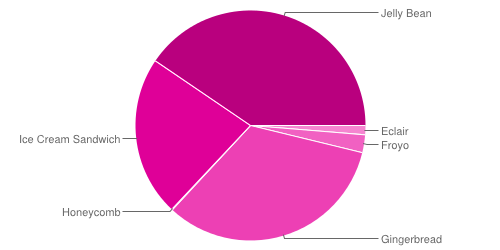
\includegraphics[scale=0.8]{./imgs/esquemas/chart.png}
\caption{Gráfico con la distribución de las versiones de la plataforma Android}
\label{fig:android_distribucion}
\end{figure}
Vemos el gráfico con la distribución de versiones de la SDK entre los dispositivos Android en la figura \ref{fig:android_distribucion}.


\begin{itemize}
  \item \emph{Honeycomb}:
    \begin{itemize} 
      \item Presenta una nueva interfaz de usuario.
      \item Gráficos acelerados por hardware.
      \item Multiselección
      \item Soportada por el 63.1\% de los dispositivos.
    \end{itemize}
    \item \emph{Ice cream Sandwich}:
    \begin{itemize} 
      \item Unificación de la interfaz de usuario.
      \item Mejora la aceleración gráfica.
      \item Mejora el soporte a múltiples pantallas. 
      \item Soportada por el 63\% de los dispositivos.
    \end{itemize}
  \item \emph{JellyBean}:
    \begin{itemize} 
      \item Simplificada la navegación.
      \item Mejora el comportamiento de los dispositivos.
      \item Mejora las notificaciones
      \item Soportada por el 40.5\% de los dispositivos.
    \end{itemize}
\end{itemize}
A la vista de esto, optamos por que la aplicación que se genera a partir de una plantilla de informe DICOM-SR fuera dirigida a Ice Cream Sandwich, puesto que ya tiene la mayor parte de las mejoras significativas de Android para tabletas y es soportada por un importante número de dispositivos.\par
Si en el futuro aparecieran mejoras que creyereamos indispensables siempre podríamos modificar las plantillas con el código  que genera la aplicación para utilizar otra versión de Android.\par


\section{Python}\label{sec:tecnologias:python}
La elección óptima de un lenguaje de programación para un proyecto determinado depende de varios factores: el equipo de desarrollo, las características del propio proyecto, las características del lenguaje\ldots\par
En este proyecto lo fundamental es la generación de código y uno de los puntos fuertes de este paradigma es que el lenguaje de programación que utilizamos para generar la aplicación y el lenguaje de la propia aplicación no tienen porque coincidir. En nuestro caso el lenguaje de la aplicación viene fijado por el problema que queremos resolver. Sin embargo podremos elegir el lenguaje para generar el código que más se adapte a nuestras necesidades.\par
Las características que debe tener un lenguaje de programación para ser apropiado para la generación de código son las siguientes \cite{herrington2003code}:
\begin{itemize}
\item Deben ser muy eficientes en la lectura, análisis gramatical y escritura de texto.
\item Deben disponer de mecanismos para crear plantillas de texto fácilmente.
\item Si soportan de manera nativa XML es útil aunque siempre se pueden incluir librerías externas para leer y manipular XML.
\item Deben ser multiplataforma.
\item La velocidad de ejecución del lenguaje no es un punto clave porque se ejecutará en producción. Es la aplicación que genere la que debe tener un buen rendimiento.
\item Su desarrollo y mantenimiento debe ser sencillo. 
\end{itemize}
\medskip\par
Pensando en todos estos puntos decidimos utilizar Python como lenguaje para generar el código de la aplicación Android.\par
Python es un lenguaje de alto nivel multipropósito y multiplataforma diseñado por Guido van Rossum en 1991. Es un lenguaje que fomenta la escritura de código legible con una sintaxis sencilla. Por su simplicidad muchas veces se utiliza como un lenguaje de scripting pero es un lenguaje suficientemente potente para utilizarlo en otros muchos contextos.\par
La implementación más común de Python esta escrita en C, se trata de CPython. Es una implementación de código abierto y gratuita, gestionada por la asociación sin ánimo de lucro  de Python (\emph{Python Software Foundation}) \cite{python}.\medskip\par
Uno de los puntos fuertes de este lenguaje es su amplia librería estándar que nos permite hacer análisis sintáctico, acceder a la API de XML, utilizar expresiones regulares, hacer uso de plantillas,\ldots de manera simple.\par
Es especialmente apropiado para este problema porque cumple todas las premisas que debe tener un buen lenguaje para la generación de código.\par
En 2009 Python lanzó su versión 3.0, la primera versión no compatible con las versiones anteriores. A pesar de que introduce un buen número de mejoras, algunas librerías externas todavía no son compatibles con esta versión. Por esto para este proyecto utilizaremos la versión 2.7 de Python. Aunque existen mecanismos \cite{py:2to3} para portar automáticamente una aplicación de Python 2.x a Python 3.x.\par
En este proyecto haremos uso de un paradigma de programación orientado a objetos, así como de las librerías estándar para gestionar la configuración, el análisis sintáctico y la parte más sencilla de las plantillas. La única librería externa que utilizaremos será Jinja, para la gestión de plantillas más complejas. Hablaremos en detalle de esto en los apartados \ref{req:implementacion}, \ref{sec:configuracion} y \ref{sec:templates}.



\chapter{Análisis}
\section{Análisis de requisitos}

Afrontamos el desarrollo de la aplicación siguiendo las pautas del esquema tradicional de desarrollo de software en cascada. Por la naturaleza del problema algunas etapas se han reducido para poder dedicar más tiempo al desarrollo de la solución.\medskip\par
En el siguiente apartado describiremos los requisitos de la solución que hemos propuesto. Durante esta fase del proyecto analizaremos las necesidades que tienen los usuarios de nuestro sistema.\par
Muchos de los requisitos vienen definidos por el propio problema y el resto por la solución que proponemos y que hemos descrito a alto nivel en el apartado \ref{solucion}. La complejidad de este proyecto estriba en la propia generación de código a partir de un fichero plantilla basada en DICOM-SR. Los casos de uso y los actores se reducen a la mínima expresión.\par
Recopilar y analizar los requisitos sienta las bases de nuestro proyecto.\par
\subsection{Requisitos funcionales}
\begin{itemize}
	\item A partir de un fichero con la plantilla de un informe médico en formato DICOM-SR, como el fichero incluido en el apéndice \ref{dicom-sr-template}, que pertenezca a una  ontología, se generarán los ficheros necesarios para instanciar una aplicación Andoid para esta plantilla que tendrá soporte para 1 o 2 idiomas en función de los idiomas que soporte el fichero DICOM.
	\item Con los ficheros generados el usuario podrá introducirlos en el esqueleto de una aplicación Android. Obteniendo una aplicación Android funcional.
	\item El entorno para la ejecución del script que genera el código y el de la aplicación esqueleto de Android deben ser fácilmente replicables, para que el usuario pueda genererar sus propias aplicaciones en distintas plataformas. 
\end{itemize}
\subsection{Requisitos no funcionales}
\begin{itemize}
\item La aplicación que genera el código debe ser lo más genérica posible para así abarcar la mayor parte de informes DICOM-SR posibles.
\item La interfaz de la aplicación se construirá mediante piezas de código intercambiables, lo que permitirá al usuario modificar la interfaz para que se acople a su metodología de trabajo.
\item La interfaz debe ser simple e intuitiva. La interfaz se construirá siguiendo un sistema de cuadrícula dónde se dará especial importancia a la tipografía y al esquema de color, para que con los mínimos elementos consigamos una interfaz de usuario amigable. 
\item El usuario podrá configurar ciertos aspectos del script que genera al código de la aplicación Android. Como por ejemplo el directorio donde estos ficheros se almacenarán, cual es el lenguaje principal, \ldots
\item La aplicación deberá facilitar la introducción de datos 
\end{itemize}
\subsection{Requisitos de implementación}\label{req:implementacion}
\begin{itemize}
\item La aplicación que genere el código se desarrollará en Python 2.7.x y seguirá las guías de estilo PEP-8 para la escritura de código y PEP-257 para la documentación.
\item La aplicación final Android se desarrollará para la versión Ice Cream Sandwich (3.2) o superior. Deberá soportar tamaños de pantalla de  10 pulgadas o más y alta resoluciones.
\item La aplicación Android se ajustará a las recomendaciones de diseño que podemos encontrar en las guías para diseñadores y desarrolladores de la web de Android Developers.
\item Se encapsularán las librerías de las que dependa el proyecto haciendo uso de \emph{virtualenv}, que permite crear entornos de desarrollo para python.
\end{itemize}
\section{Actores}\label{sec:actores}
En la tabla \ref{actores}, podemos ver la definición formal de los usuarios que emplearán el sistema que vamos a desarrollar. \par
Únicamente tenemos un actor y un caso de uso, que veremos en el apartado \ref{sec:casos-uso}, porque la generación de código debe necesitar la mínima interacción de los usuarios. Sin embargo por coherencia con la metodología de desarrollo realizamos el modelado de los actores y de los casos de uso.\par

\begin{table}
\begin{center}
  
  \begin{tabular}{ |b{4cm}||b{3cm}|b{1cm}|b{2cm}|b{1.5cm}| b{1cm}| }
    \hline
    \cellcolor{RubineRed} {\color{White} Actor} & \multicolumn{2}{|l|}{Usuario}  & \multicolumn{2}{|l|}{\color{RubineRed} Identificador}  &  USER1 \\ 
    \hline \hline
    {\color{RubineRed} Descripción } & \multicolumn{5}{|l|}{Usuario que generará automáticamente aplicaciones Android.}  \\ 
    \hline
    {\color{RubineRed} Características } & \multicolumn{5}{|l|}{\parbox{10.5cm}{El usuario dispondrá del entorno python  y de las aplicación esqueleto de Android, así como de un fichero con la plantilla de un informe DICOM-SR.}} \\ 
    \hline
    {\color{RubineRed} Relaciones } & \multicolumn{5}{|l|}{}\\ 
    \hline
    {\color{RubineRed} Referencias } &  \multicolumn{5}{|l|}{CONF,GENCOD,INSAND}\\ 
    \hline
    {\color{RubineRed} Autor } &  Mayte Giménez & {\color{RubineRed} Fecha } & 16/08/2013 & {\color{RubineRed} Version } & v1.0 \\ 
    \hline
    \end{tabular}
    \begin{tabular}{ |b{4cm}|b{6cm}|b{4.75cm}|}
    \hline
    \multicolumn{3}{|>{\columncolor{RubineRed}}l|}{\color{White}  Atributos} \\
    \hline
    {\color{RubineRed} Nombre } & {\color{RubineRed} Descripción } & {\color{RubineRed} Tipo} \\
    \hline
    Vacío & Vacío & Vacío \\
    \hline
    \end{tabular}
    \begin{tabular}{ |b{15.6cm}|}
    \hline
    \cellcolor{RubineRed} {\color{White} Comentarios}  \\
    \hline
	\parbox{15.5cm}{Aunque para ejecutar la aplicación el usuario no requiera ningún tipo de conocimiento del sistema generador de código o de los informes médicos, el usuario debe disponer de un fichero plantilla basado en DICOM-SR correctamente elaborado. Además debe de tener la aplicación esqueleto Android para instanciar la aplicación final. Además debe disponer de un dispositivo Android con la versión 3.2 o superior.}    \\
	\hline

    \end{tabular}
\end{center}
	\caption{Actores del sistema}
	\label{actores}
\end{table}
\newpage
\section{Casos de uso}\label{sec:casos-uso}
\renewcommand*{\arraystretch}{1.5}
%\begin{table}
\begin{center}
  \begin{longtable}{ |b{2.5cm}|b{4cm}|b{1cm}|b{2cm}|b{1.5cm}| b{2.5cm}| }
  
    \hline
    \cellcolor{RubineRed} {\color{White} Caso de uso} & \multicolumn{2}{|l|}{\parbox{4.5cm}{Configuración del generador de código}}  & \multicolumn{2}{|l|}{\color{RubineRed} Identificador}  &  CONF \\ 
    \hline \hline
    {\color{RubineRed} Actores } & \multicolumn{5}{|l|}{Usuario}  \\ 
    \hline
    {\color{RubineRed} Tipo } & \multicolumn{5}{|l|}{Primario}  \\ 
    \hline
    {\color{RubineRed} Referencias } & \multicolumn{5}{|l|}{}  \\ 
    \hline
    {\color{RubineRed} Precondición } & \multicolumn{5}{|l|}{\parbox{13cm}{El usuario dispone de un fichero para generar la aplicación que sigue el estándar DICOM-SR. Y tiene el entorno de desarrollo para la aplicación generadora de código preparado.} }  \\ 
    \hline
    {\color{RubineRed} Postcondición } & \multicolumn{5}{|l|}{\parbox{13cm}{Los ficheros de configuración del generador quedarán personalizados según las necesidades del usuario.}}  \\ 
    \hline
    {\color{RubineRed} Autor } &  Mayte Giménez & {\color{RubineRed} Fecha } & 16/08/2013 & {\color{RubineRed} Version } & v1.0 \\ 
    \hline
    {\color{RubineRed} Propósito } & \multicolumn{5}{|l|}{\parbox{13cm}{Configurar las opciones parametizables del generador de código de la aplicación Android.}}  \\ 
    \hline
    \multicolumn{6}{|l|}{{\color{RubineRed} Resumen }}  \\ 
    \hline
   	\multicolumn{6}{|l|}{\parbox{16cm}{ Existen un número de opciones que el usuario puede modificar como son: las cadenas de texto que aparecen en los idiomas soportados, la ruta dónde se creará el código generado automáticamente y las ontologías soportadas. Los ficheros de configuración permiten que el usuario edite estas opciones para que el código generado se adapte a sus necesidades.}}  \\ 
    \hline
    \multicolumn{6}{|l|}{\parbox{8cm}{{\color{RubineRed} Curso normal }}}  \\ 
    \hline
    1 & \multicolumn{2}{|l|}{\parbox{5cm}{ El usuario modifica alguno o varios de los parámetros de configuración}} &  & \multicolumn{2}{|l|}{}\\
    \hline
     & \multicolumn{2}{|l|}{} & 2 &  \multicolumn{2}{|l|}{\parbox{5cm}{El sistema lee la configuración y cuando el usuario ejecute el script de generación de código aplicará las modificaciones.}}\\
    \hline
    \multicolumn{6}{|l|}{\parbox{8cm}{{\color{RubineRed} Curso alterno }}}  \\ 
    \hline
    2b & \multicolumn{5}{|l|}{\parbox{13cm}{Si alguno de los parámetros de configuración no es válido, este volverá al valor por defecto.}}  \\ 
    \hline
    \caption{Casos de uso: Configuración del generador de código}
  	\label{tab:caso-uso:conf}
    \end{longtable}
\end{center}
%\end{table}

\begin{center}
  \begin{longtable}{ |b{2.5cm}|b{4cm}|b{1cm}|b{2cm}|b{1.5cm}| b{2.5cm}| }
    \hline
    \cellcolor{RubineRed} {\color{White} Caso de uso} & \multicolumn{2}{|l|}{\parbox{4.5cm}{Generación del código de la aplicación Android}}  & \multicolumn{2}{|l|}{\color{RubineRed} Identificador}  &  GENCOD \\ 
    \hline \hline
    {\color{RubineRed} Actores } & \multicolumn{5}{|l|}{Usuario}  \\ 
    \hline
    {\color{RubineRed} Tipo } & \multicolumn{5}{|l|}{Primario}  \\ 
    \hline
    {\color{RubineRed} Referencias } & \multicolumn{5}{|l|}{}  \\ 
    \hline
    {\color{RubineRed} Precondición } & \multicolumn{5}{|l|}{\parbox{13cm}{El fichero para generar la aplicación debe seguir el estándar DICOM-SR y pertenecer a las ontologías soportadas en la configuración.} }  \\ 
    \hline
    {\color{RubineRed} Postcondición } & \multicolumn{5}{|l|}{\parbox{13cm}{Se generarán los ficheros necesarios para instanciar la aplicación Android esqueleto.}}  \\ 
    \hline
    {\color{RubineRed} Autor } &  Mayte Giménez & {\color{RubineRed} Fecha } & 16/08/2013 & {\color{RubineRed} Version } & v1.0 \\ 
    \hline
    {\color{RubineRed} Propósito } & \multicolumn{5}{|l|}{\parbox{13cm}{ Generar parte del código necesario de una aplicación Android.}}  \\ 
    \hline
    \multicolumn{6}{|l|}{{\color{RubineRed} Resumen }}  \\ 
    \hline
   	\multicolumn{6}{|l|}{\parbox{16cm}{El usuario ejecutará el script pasándole el fichero plantilla basado en DICOM-SR y el método de internacionalización de este fichero (i18n o default) y el sistema generará los ficheros de código necesarios para instanciar la aplicación Android.}}  \\ 
    \hline
    \multicolumn{6}{|l|}{\parbox{8cm}{{\color{RubineRed} Curso normal }}}  \\ 
    \hline
   	1 & \multicolumn{2}{|l|}{\parbox{5cm}{ El usuario ejecuta el script generador de código. Los argumentos serán el fichero plantilla basado en DICOM-SR y el método de internacionalización}} &  & \multicolumn{2}{|l|}{}\\
    \hline
    & \multicolumn{2}{|l|}{} & 2 & \multicolumn{2}{|l|}{\parbox{5cm}{El sistema comprueba que el fichero existe y que el método de internacionalización es correcto}}\\
    \hline
     & \multicolumn{2}{|l|}{} & 3 &  \multicolumn{2}{|l|}{\parbox{5cm}{El sistema realiza el análisis sintáctico del fichero DICOM-SR}}\\
    \hline
    & \multicolumn{2}{|l|}{} & 4 &  \multicolumn{2}{|l|}{\parbox{5cm}{El sistema carga en una estructura de árbol la información del fichero DICOM-SR}}\\
    \hline
    & \multicolumn{2}{|l|}{} & 5 &  \multicolumn{2}{|l|}{\parbox{5cm}{El sistema genera las cadenas de internacionalización necesarias para la aplicación Android}}\\
    \hline
    & \multicolumn{2}{|l|}{} & 6 &  \multicolumn{2}{|l|}{\parbox{5cm}{El sistema genera los ficheros XML para la interfaz de usuario.}}\\
    \hline
    & \multicolumn{2}{|l|}{} & 7 &  \multicolumn{2}{|l|}{\parbox{5cm}{El sistema genera las clases Java que modelan el informe médico}}\\
    \hline
    & \multicolumn{2}{|l|}{} & 8 &  \multicolumn{2}{|l|}{\parbox{5cm}{El sistema genera las clases Java que controlan la aplicación Android.}}\\
    \hline
    & \multicolumn{2}{|l|}{} & 9 &  \multicolumn{2}{|l|}{\parbox{5cm}{El sistema genera el manifiesto de la aplicación Android.}}\\
    \hline
    \multicolumn{6}{|l|}{\parbox{8cm}{{\color{RubineRed} Curso alterno }}}  \\ 
    \hline
    2b & \multicolumn{5}{|l|}{\parbox{13cm}{Si el sistema detecta que el método de internacionalización no es correcto usará el método por defecto, descartando la información del segundo idioma si existiera}}  \\ 
        \hline
    5b & \multicolumn{5}{|l|}{\parbox{13cm}{Si los ficheros XML de las cadenas de internacionalización ya existen en la ruta especificada no se vuelven a generar.}}  \\ 
    \hline
    6b & \multicolumn{5}{|l|}{\parbox{13cm}{Si los ficheros XML de la interfaz de usuario ya existen en la ruta especificada no se vuelven a generar.}}  \\ 
	\hline
    7b & \multicolumn{5}{|l|}{\parbox{13cm}{Si los ficheros Java con el modelo ya existen en la ruta especificada no se vuelven a generar.}}  \\
	\hline
	8b & \multicolumn{5}{|l|}{\parbox{13cm}{Si los ficheros Java que controlan la aplicación Android ya existen en la ruta especificada no se vuelven a generar.}}  \\
	\hline
	9b & \multicolumn{5}{|l|}{\parbox{13cm}{Si el manifiesto Android ya existe en la ruta especificada no se vuelven a generar.}}  \\
	\hline
    \caption{Casos de uso: Generación de código}
  	\label{tab:casos-uso:gen}
    \end{longtable}
\end{center}

\begin{center}
  \begin{longtable}{ |b{2.5cm}|b{4cm}|b{1cm}|b{2cm}|b{1.5cm}| b{2.5cm}| }
    \hline
    \cellcolor{RubineRed} {\color{White} Caso de uso} & \multicolumn{2}{|l|}{\parbox{4.5cm}{Instanciación de la aplicación Android}}  & \multicolumn{2}{|l|}{\color{RubineRed} Identificador}  &  INSAND \\ 
    \hline \hline
    {\color{RubineRed} Actores } & \multicolumn{5}{|l|}{Usuario}  \\ 
    \hline
    {\color{RubineRed} Tipo } & \multicolumn{5}{|l|}{Primario}  \\ 
    \hline
    {\color{RubineRed} Referencias } & \multicolumn{5}{|l|}{}  \\ 
    \hline
    {\color{RubineRed} Precondición } & \multicolumn{5}{|l|}{\parbox{13cm}{El usuario dispone de los ficheros generados a partir de un fichero plantilla basado DICOM-SR y la estructura de la aplicación Android que los contendrá.} }  \\ 
    \hline
    {\color{RubineRed} Postcondición } & \multicolumn{5}{|l|}{\parbox{13cm}{Se crea una aplicación Android para el informe médico DICOM-SR a partir del cual se habían generado los ficheros.}}  \\ 
    \hline
    {\color{RubineRed} Autor } &  Mayte Giménez & {\color{RubineRed} Fecha } & 16/08/2013 & {\color{RubineRed} Version } & v1.0 \\ 
    \hline
    {\color{RubineRed} Propósito } & \multicolumn{5}{|l|}{\parbox{13cm}{Disponer de una aplicación Android que permita al usuario introducir los datos de informes DICOM-SR de la ontología instanciada.}}  \\ 
    \hline
    \multicolumn{6}{|l|}{\parbox{8cm}{{\color{RubineRed} Resumen }}}  \\ 
    \hline
   	\multicolumn{6}{|l|}{\parbox{16cm}{ Con el esqueleto de la aplicación Android para este proposito y todos los ficheros necesarios para personalizarla, el sistema instancia la aplicación Android para esta plantilla específica.}}  \\ 
    \hline
    \multicolumn{6}{|l|}{\parbox{8cm}{{\color{RubineRed} Curso normal }}}  \\ 
    \hline
    1 & \multicolumn{2}{|l|}{\parbox{5cm}{El usuario llama al script con la ruta raíz dónde se encuentran los ficheros generados y la ruta raíz de la aplicación Android.}} &  & \multicolumn{2}{|l|}{\parbox{5cm}{ El sistema comprueba que los ficheros generados y la aplicación Android esqueleto existan.}}\\
    \hline
     & \multicolumn{2}{|l|}{} & 3 &  \multicolumn{2}{|l|}{\parbox{5cm}{El sistema copia los ficheros en la ruta que les corresponde dentro de la aplicación Android.}}\\
    \hline
    \multicolumn{6}{|l|}{\parbox{8cm}{{\color{RubineRed} Curso alterno }}}  \\ 
    \hline
    2b & \multicolumn{5}{|l|}{\parbox{13cm}{Si alguna de las rutas no existe o falta algún fichero necesario la ejecución se aborta.}}  \\ 
    \hline
    \caption{Casos de uso: Instanciación de la aplicación Android}
  	\label{tab:casos-uso:android}
    \end{longtable}
\end{center}

\chapter{Diseño}

\section{Arquitectura de la solución}
En este apartado continuaremos profundizando en los detalles de la solución propuesta en el apartado \ref{solucion}. Describiremos tanto la arquitectura de la aplicación generadora del código como de la aplicación esqueleto de Android que instanciaremos con la plantilla de un informe DICOM-SR.\par

\subsection{Aplicación Android}
Nuestro objetivo último es disponer de una aplicación Android para una determinada ontología de informe médico,  que facilite al personal clínico la tarea de rellenar los informes de los pacientes siguiendo el estándar DICOM-SR. Por lo tanto el código que generaremos deberá contener todos los componentes de una aplicación Android.

\subsubsection{Justificación para desarrollar un aplicación nativa para Android}

En este proyecto generamos una aplicación nativa para Android. Antes de entrar en profundidad a describir la anatomía de una aplicación Android, dedicaremos unas líneas a justificar la decisión de escribir una aplicación nativa para Android en lugar de desarrollar una aplicación genérica en HTML5, o utilizando frameworks como Phonegap \cite{phonegap}, Titanium \cite{titanium} o Corona \cite{corona} para crear una aplicación híbrida, o ya que nuestro generador de código está escrito en Python porque no utilizar Python también en Android mediante el framework Kivy\cite{kivy}.\medskip\par

Comenzaremos por argumentar esta última opción ya que es también la más sencilla de rebatir. Que escribamos el generador de código en un lenguaje no implica que el software generado deba estar escrito en ese mismo lenguaje, de hecho esta disociación es un punto fuerte de la generación de código, como ya explicamos en el apartado \ref{sec:generacion-codigo}.\par 
La utilización de Kivy está justificada cuando queremos hacer una aplicación multiplataforma, para dispositivo móviles y de escritorio, sin necesidad de reescribir del código. Aporta la potencia y simplicidad de Python y está recomendado para el desarrollo de juegos o aplicaciones con gran carga gráfica, ya que en el caso de aplicaciones genéricas la interfaz que crea este framework no es la más apropiada.\par
En nuestro caso, la aplicación final es un formulario,  y una de las premisas que nos hemos marcado es que sea intuitiva y fácil de utilizar, por lo tanto los elementos de la interfaz no deberán sorprender al usuario y la interacción con el usuario debe ser ágil. Como generar código en Python supone el mismo esfuerzo que generarlo en cualquier otro lenguaje y no nos ofrece ventajas adicionales descartamos esta opción.\medskip\par

La siguiente opción sería desarrollar una aplicación en HTLM5.\par
Las ventajas principales que tiene esta opción es la rapidez en el desarrollo y que no es necesario pasar un proceso de validación de la misma. Por otra parte se resiente la velocidad de ejecución y no se tiene acceso a todas las funcionalidades de los teléfono o tabletas para las que se desarrolla.\par 
No vamos a necesitar funcionalidades complejas pero el hecho de que la velocidad de ejecución se reduzca respecto a las aplicaciones nativas empeora la usabilidad y por tanto el índice de aceptación de los usuarios y este si es un punto relevante para nuestro objetivo, por lo tanto también descartamos esta opción.\medskip\par

Finalmente quedaría la opción de desarrollar una aplicación híbrida.\par
Esta opción puede hacer uso de las funcionalidades de las tabletas y puede funcionar a la misma velocidad que una aplicación nativa, además tiene aporta el beneficio de que las aplicaciones sobre estos frameworks son más sencillas de desarrollar, pero aportan las complicaciones propias de instalar y trabajar con el framework.\par
Nuestro objetivo es que con un fichero DICOM-SR se genere de automáticamente una aplicación Android. El esqueleto de la aplicación en Android podemos tenerlo preparado e instanciar la aplicación para el fichero concreto, en cambio incluir un framework introduce un nivel más que nos complica la generación automática. Y respecto a la complicación del desarrollo, como el código que generamos lo hacemos mediante generación automática guiada por modelos, desarrollar una aplicación en Anroid no implica un esfuerzo mucho mayor que hacerlo para algún framework para aplicaciones híbridas.\medskip\par

Por lo tanto la opción que más se adapta a las necesidades concretas de este proyecto es el desarrollo de una aplicación nativa para Android.\par

\subsubsection{Esquema de una aplicación Android}
Las aplicaciones Android las aplicación siguen normalmente el patrón de desarrollo Modelo-Vista-Controlador(MVC).
%, o siendo más específicos el patrón de desarrollo Modelo-Vista-Presentador (MVP) que es una evolución del anterior. 
El modelo y los presentadores o controladores se programan en Java y para definir la interfaz de usuario se utilizan ficheros XML.\par
Una aplicación que sigue este patrón de diseño se compone por:
\begin{itemize}
\item \textbf{Vista}: Contiene la interfaz de usuario y las cadenas de texto para internacionalizar dicha interfaz.\par
\item \textbf{Modelo}: Es la información del sistema, encapsula el estado del sistema. 
\item \textbf{Controlador}: Responde a los eventos generados por la vista y interactua con el modelo. 
\end{itemize}

\begin{figure}[ht]
\centering
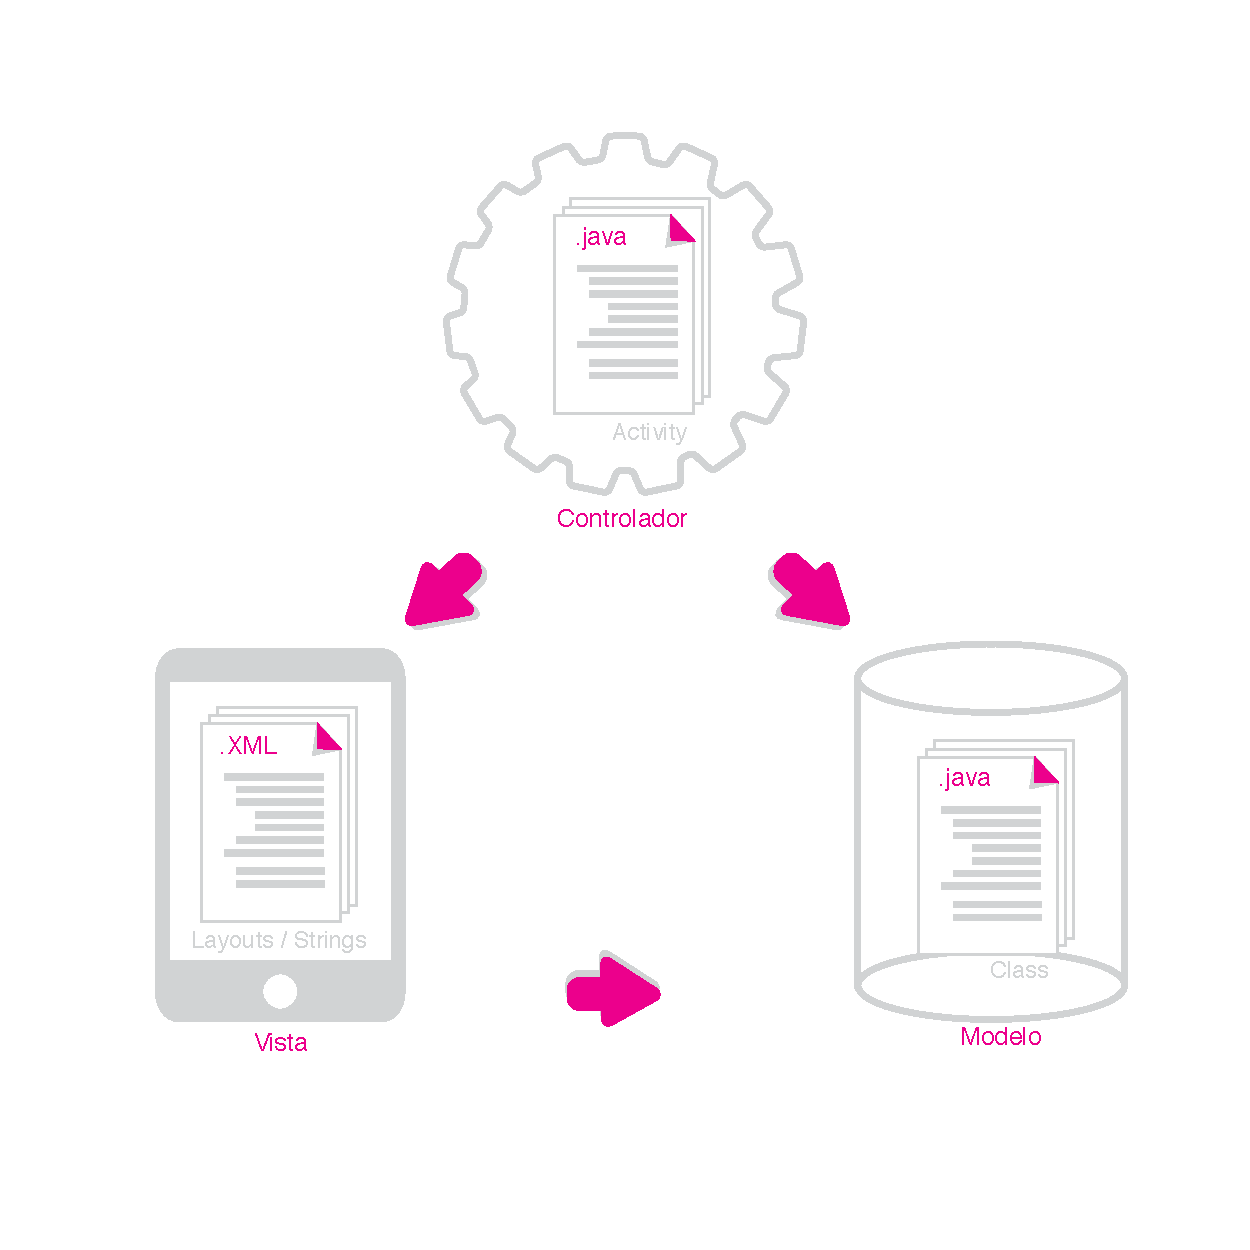
\includegraphics[scale=0.5]{./imgs/esquemas/mvc.pdf}
\caption{Generación parcial de clases}
\label{fig:mvc}
\end{figure}

En la figura \ref{fig:mvc}, vemos el esquema del patrón de desarrollo MVC aplicado en una aplicación Android.\par
Las partes de las que se compone una aplicación Android son las siguientes:
\begin{itemize}
\item \textbf{Vista}: La vista de la aplicación se desarrolla mediante ficheros XML. La vista en Android se compone fundamentalmente por dos elementos: los ficheros XML que definen la interfaz de usuario, que podemos encontrar en \emph{\textbackslash{res}\textbackslash{layout}} y por otra parte tenemos los ficheros XML con las cadenas de texto que se utilizarán en la interfaz, correctamente internacionalizadas y almacenadas en \emph{\textbackslash{res}\textbackslash{values}}. Adicionalmente se puede definir estilos para los elementos de la interfaz gráfica, análogamente a como se hace en CSS, estos ficheros de estilo los podemos encontrar también en \emph{\textbackslash{res}\textbackslash{values}}. Para soportar distintos tipos de pantalla en Android, las imágenes y los estilos se organizan dentro de carpetas determinadas en la aplicación Android y en función de la resolución del dispositivo se cargarán unas u otras.
\item \textbf{Modelo}: El modelo en para una aplicación Android no difiere del modelo en otro lenguaje. Se trata de una serie de clases con la información del sistema. En nuestro caso serán las clases que contengan la información del informe médico. Encapsularemos el modelo dentro del paquete \emph{model}.
\item \textbf{Controlador}: Finalmente los controladores en las aplicaciones Android son las Actividades (\emph{Activity}). Las actividades gestionan la interfaz de usuario, interactuan con el usuario y acceden al modelo bien para mostrarlo en la vista o para modificarlo. 
\end{itemize}

Finalizaremos este apartado viendo la estructura de ficheros de la aplicación Android que nos servirá como framework para instanciar las aplicaciones concretas sobre un informe DICOM-SR y señalando las rutas dónde irán los ficheros que generaremos.\par

\begin{figure}
\centering
\framebox[1.05\textwidth]{%
\begin{minipage}{0.95\textwidth}
	\dirtree{%
		.1 meer-framework/.
		.2 {\color{RubineRed} AndroidManifest.xml.}
		.2 assets/. 
		.3 \vdots.
		.2 bin/. 
		.3 \vdots.
		.2 gen/. 
		.3 \vdots.
		.2 libs/. 
		.3 \vdots.
		.2 src/.
		.3 com/.
		.4 i3m/.
		.5 meer/.
		.6 {\color{RubineRed} *.java }\DTcomment{\emph{Actividades}}.
		.6 model/.
		.7 {\color{RubineRed} *.java }\DTcomment{\emph{Modelo}}.
		.2 res/.
		.3 drawable-hdpi/.
		.4 \vdots\DTcomment{\emph{Iconos e imágenes para alta resolución (> 640dp x 480dp)}}.
		.3 drawable-ldpi/.
		.4 \vdots\DTcomment{\emph{Iconos e imágenes para baja resolución (> 426dp x 320dp)}}.
		.3 drawable-mdpi/.
		.4 \vdots\DTcomment{\emph{Iconos e imágenes para resolución media (> 470dp x 320dp)}}.
		.3 drawable-xhdpi/.
		.4 \vdots\DTcomment{\emph{Iconos e imágenes para extra alta resolución (> 960dp x 720dp)}}.
		.3 layout/.
		.4 {\color{RubineRed} *.xml }\DTcomment{\emph{Vista: UI}}.
		.2 menu/. 
		.3 \vdots\DTcomment{\emph{Vista: menús}}.
		.2 values/. 
		.3 {\color{RubineRed} *.xml }\DTcomment{\emph{Vista: estilos y cadenas de texto}}.
		.2 values-11/. 
		.3 {\color{RubineRed} *.xml }\DTcomment{\emph{Vista: estilos para API 11}}.
		.2 values-14/. 
		.3 {\color{RubineRed} *.xml }\DTcomment{\emph{Vista: estilos para API 14}}.
	}
\end{minipage}
}
\caption{Estructura de ficheros de la aplicación framework Android}
\end{figure}

\subsection{Aplicación generadora de código}
\subsubsection{Diagrama de clases}


\section{Diseño de interfaces}

\section{Prototipo}

\chapter{Implementación}
\section{Entorno de trabajo}

A continuación describiremos brevemente el entorno de trabajo que hemos empleado para desarrollar el proyecto y que debemos hacer para reproducir este entorno de desarrollo.\par
Hemos trabajado indistintamente sobre sistemas operativos basados en Unix, utilizando Mac OS X y Linux; pero el entorno podría reproducirse para trabajar también sobre Windows.\par
Aunque se trata de un proyecto individual, el código se mantenía bajo un sistema de control de versiones, lo que permite mantener un registro histórico del desarrollo. Mantendremos dos repositorios en Github: uno en el que mantendremos el diseño del framework de Android \cite{meer:android} y otro para desarrollar el generador de código \cite{meer}.\par

\subsection{Python}
La aplicación que genera el código está escrita en Python, así que obviamente necesitaremos el intérprete de Python para poder ejecutarla.\par
Emplearemos la rama 2.x de Python por los motivos que justificamos en el aparado \ref{sec:tecnologias:python}. En las plataformas en las que hemos estado desarrollando podemos encontrar Python en la versión 2.7, la última versión estable del lenguaje, y es sobre esta versión sobre la que trabajaremos.\par

\subsubsection{Pip y VirtualEnv}\label{sec:virtualenv}
Uno de los problemas más comunes en el desarrollo son los conflictos entre librerías y la necesidad de replicar entornos de trabajo.\par 
En Python existen dos herramientas que permiten atajar este problema: pip y virtualenv. \par
Pip es una herramienta para instalar y gestionar paquetes de Python automáticamente. Instalar un paquete con pip es tan sencillo como indicar el nombre del paquete y la versión, como vemos en el ejemplo de código \ref{pip}.\par

\begin{lstlisting}[language=bash,label=pip,caption=Instalación de un paquete utilizando pip]
	$ pip install SomePackage==1.0  
\end{lstlisting}

También acepta como parámetro para instalar paquetes un fichero las librerías del proyecto, como podemos ver en el ejemplo de código \ref{pip-req}.\par

\begin{lstlisting}[language=bash,label=pip-req,caption=Instalación de los requisitos de un proyecto utilizando pip]
	$ pip install requirements.txt  
\end{lstlisting}

Para conocer las dependencias de un proyecto únicamente tendremos que ejecutar pip con el parámetro \emph{freeze} y nos devolverá un listado con las librerías que necesita este proyecto, que guardaremos en un fichero requirements.txt, lo que nos permitirá replicar el entrono fácilmente. \par
En esta aplicación únicamente hacemos uso de la librería externa Jinja2, y esta a su vez necesita MarkupSafe y wsgiref. Así que el fichero con los requisitos será como el que vemos en el código de \ref{requisitos}.\par

\begin{lstlisting}[language=bash,label=requisitos,caption=Requisitos del proyecto]
	Jinja2==2.7
	MarkupSafe==0.18
	wsgiref==0.1.2
\end{lstlisting}


La otra herramienta de la que haremos uso es virtualenv  que  crea entornos virtuales de Python aislados evitando los conflictos de dependencias entre las librerías de un proyecto y permite replicar el entorno fácilmente.\par
Cada entrono virtual contiene su propia versión de Pip encapsuladas. Lo que permite instalar librerías dentro del entorno que hayamos creado.\medskip\par

La combinación de estos dos paquetes nos permite tener entornos de trabajo con todas las dependencias del proyecto que pueden ser replicados con facilidad. 

\subsection{Android}

Tanto para desarrollar el prototipo como para crear el framework de Android que instanciará los informes DICOM-SR, necesitamos trabajar dentro del entorno de desarrollo de Android.\par
Para desarrollar una aplicación haremos uso de las siguientes herramientas:
\begin{itemize}
\item El kit de desarrollo de Java (JDK).	
\item La kit de desarrollo de  Android (Android SDK). En nuestro caso necesitaremos la SDK de la versión 3.2.
\item El IDE de desarrollo Eclipse.
\item El plugin para Eclipse para poder trabajar con Android. (ADT)
\end{itemize}

\medskip\par
Concluyendo, tenemos un entrono de trabajo para el generador de código y otro para el desarrollo de la aplicación framework de Android. Esto nos permite desarrollar de modo independiente cada una de las partes que componen la arquitectura de la solución.


\section{Aplicación framework de Android}
El desarrollo de la solución final sigue la metodología en cascada. Pero necesitamos desarrollar simultáneamente una aplicación Android que nos servirá como esqueleto (o framework) para insertar en ella el código que generemos a partir de un informe DICOM-SR concreto.\par 
Para esta aplicación Android necesitamos que el usuario valide las decisiones de diseño e interacción que hemos tomado, por lo tanto ya durante la etapa de diseño elaboramos un prototipo como ya hemos explicado en el apartado \ref{prototipo}.\par

Este mismo prototipo lo haremos evolucionas para que nos sirva como esqueleto para las aplicaciones generadas. Simplemente eliminaremos del prototipo todas las partes que correspondan a un informe concreto, y las sustituiremos por el código generado automáticamente. Y añadiremos las funcionalidades que sean genéricas para todas las aplicaciones que se generan a partir de informes DICOM-SR. \medskip\par

Durante el desarrollo de este prototipo nos dimos cuenta que algunas de las pantallas diseñadas en la etapa anterior no podían generalizarse fácilmente. Por ejemplo, en las figuras  \ref{fig:mockup:tree} y \ref{fig:mockup:treenodes}  veíamos todas las posibles lesiones de todos los órganos de este informe como no siempre habrán dos órnagos involucrados en un informe, esta pantalla no podía generalizarse.\par
Decidimos entoces ordenar las pantallas siguiendo la estructura propia del informe. Si bien la solución propuesta en el apartado \ref{sec:ui-mockup} agrupa el conocimiento de una forma algo más simple para el usuario final que únicamente sirva para un subconjunto de informes médicos hace que la descartemos. Optando por una solución genérica que permita transformar en una aplicación Android cualquier plantilla de informe médico.\medskip\par  

Para no duplicar información, podremos ver las modificaciones realizadas en la aplicación esqueleto en el apartado \ref{sec:appfinal}.\par
Resumiendo hemos evolucionado el prototipo desarrollado en la etapa anterior para poder instanciar todo tipo de infores médicos. De esta aplicación Android, eliminamos los fragmentos que pertenecen a un informe concreto quedándonos el esqueleto que después completaremos con el código generado automáticamente. 


\section{Analizador sintáctico}
El análisis sintáctico (parsing) se encarga de leer el fichero de tipo DICOM-SR y crear una estructura de datos en memoria con la información del fichero. La estructura de datos más comúnmente empleada para esta tarea es un  árbol ya que encapsula la información tanto de los nodos como de la jerarquía.\medskip\par

Los analizadores sintácticos de XML se dividen en dos categorías fundamentalmente \cite{li2009xml}: analizadores DOM (Document Object Model) y SAX (Simple API for XML).\par
DOM emplea es una interfaz de aplicación (API) basada en árbol que modela todo el documento XML como un árbol. Es adecuado cuando queremos realizar operaciones sobre ficheros complejos y sobre los que realizan accesos aleatorios, porque en el árbol generado tenemos toda la información del informe. Pero este árbol que genera puede llegar a ser hasta 10 veces más grande que el fichero XML lo hace poco apropiado para tratar con ficheros grandes.\par
SAX, por el contrario es una interfaz de aplicación basada en eventos. Lee el fichero secuencialmente, cada nodo leído provocará que se lance un evento que es tratado por el analizador de tipo SAX. SAX es apropiado para ficheros grandes, porque según va leyendo el fichero lanzará los eventos asociados y descarta la información de lo leído hasta este punto. Su complejidad espacial es menor porque no necesita almacenar mucha información en memoria. Precisamente por este motivo no permite realizar operaciones que requieran de información global.\par
En nuestro caso, los informes DICOM-SR con los que trabajamos son potencialmente muy largos, por lo que un análisis tipo DOM queda descartado. Sin embargo, para generar el código necesitaremos un árbol, lo que haremos tras el análisis es generar una estructurea arbórea eficiente. Este proceso se describe en el apartado \ref{sec:better_tree}.\medskip\par

En la librería estándar de Python podemos encontrar el paquete \emph{xml.sax}, que implementa la interfaz de SAX.\par
Como en nuestro caso queremos extender el comportamiento del analizador sintáctico XML para que sea capaz de interpretar ficheros con plantillas de informes médicos DICOM-SR, por lo tanto crearemos una clase que extienda de la clase \emph{xml.sax.ContentHandler} que es precisamente la clase que trata los eventos lanzados por el analizador sintáctico.\medskip\par

En la figura \ref{fig:uml-parser} hemos visto el diagrama UML que modela esta clase.\par
Los atributos internos nos permiten almacenar información acerca de lo leído en el fichero y al terminar el análisis generar un árbol con los datos del informe DICOM-SR.\par

En el segmento de código \ref{DicomParser} vemos como la clase \emph{DicomPasrser} extiende del analizador sintáctico SAX estándar. Recibe un informe DICOM-SR que sigue el formato XML y en la variable interna \emph{self.\_dict\_report} devolverá la estructura arbórea eficiente con la información del fichero DICOM-SR.\par

\lstset{escapechar=@,style=python}
\begin{lstlisting}[label=DicomParser,caption=Clase que analiza sintácticamente un fichero DICOM-SR]
class DicomParser(xml.sax.handler.ContentHandler):
    ...

    def parse(self, xml_file):
        """ Parse the file using this handler.
        Returns the report using a DictReporT.

        Keyword Argument:
        xml_file  -- XML file in DICOM format to parse

        """
        xml.sax.parse(xml_file, self)
        return self._dict_report
    ...
\end{lstlisting}

Los métodos que hemos sobrecargado para recoger información del informe DICOM-SR son los siguientes:
\begin{itemize}
\item \emph{startElement}: es llamado cada vez que un nueva etiqueta de apertura de un nodo. En nuestro caso lo empleamos para iniciar variables y preparar las variables que nos indican en que punto del análisis sintáctico nos encontramos.
\item \emph{endElement}: se llama cuando se encuentra un final de etiqueta. Si se trata del final de un atributo, almacenamos la información en un contenedor temporal de tipo \emph{SAXContainer} y si se trata del final del contenedor en si, lo añadimos a la variable interna de tipo \emph{SAXReport} que guarda una lista con todos los contenedores DICOM-SR encontrados. 
\item \emph{characters}: se llama cada vez que se lee un carácter y este es almacenado en un buffer.
\item \emph{endDocument}: finalmente cuando termina el documento se llama este método. Como en este punto ya tenemos toda la información del fichero, la reorganizaremos en forma de árbol. Este proceso lo explicaremos en el apartado \ref{sec:better_tree}.
\end{itemize}\medskip\par

En los informes DICOM-SR, cada contenedor sigue un formato estándar lo que le da gran versatilidad. En un contenedor DICOM-SR sus atributos y los contenedores que cuelgan de este contenedor se agrupan bajo la etiqueta de los hijos.Por simplicidad para generar el código, hemos agrupado los atributos dentro del contenedor y sus hijos serán únicamente otros contenedores.\par
En la figura \ref{fig:SAXReport_schema} vemos un esquema de cómo se estructura la información en el analizador sintáctico, al compararla figura \ref{fig:dicom-report} encontramos las diferencias que hemos descrito respecto a un fichero DICOM-SR.\par

\begin{figure}[ht]
\centering
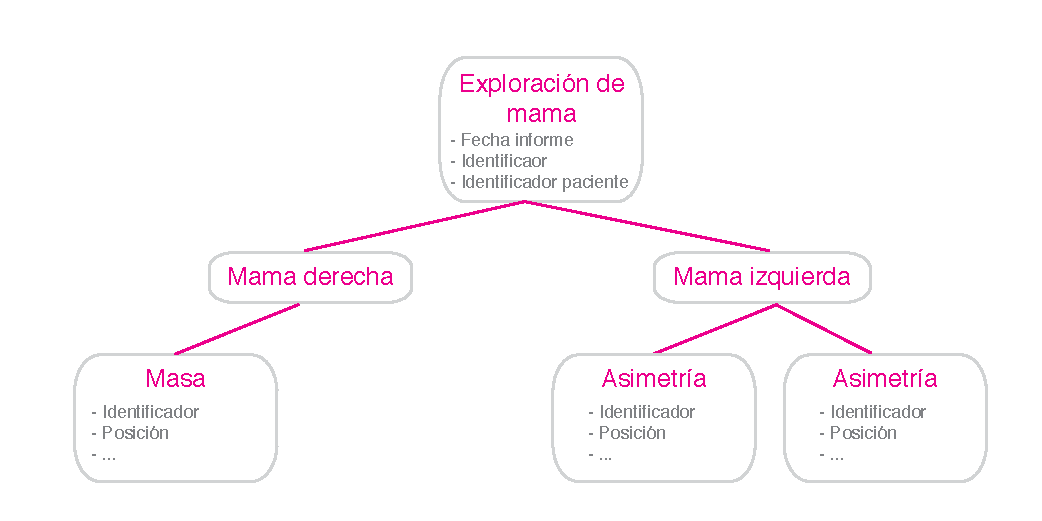
\includegraphics[scale=0.7]{./imgs/esquemas/dicomsrTreeSAX.pdf}
\caption{Esquqema del árbol DICOM-SR para el analizador sintáctico}
\label{fig:SAXReport_schema}
\end{figure}


Para almacenar la información a medida que vamos leyendo creamos dos clases: \emph{SAXContainer} y \emph{SAXReport}.\par
En el segmento de código \ref{SAXContainer} vemos la interfaz de la clase desarrollada para almacenar y gestionar los contenedores DICOM-SR mientras se está leyendo el fichero. Como ya hemos explicado los atributos DICOM-SR se integran dentro del contenedor. Además hemos definido atributos como \emph{open}, \emph{parent} y \emph{tree\_level} para almacenar elementos de la estructura del informe que nos permitirán después construir el árbol.\par

\begin{lstlisting}[label=SAXContainer,caption=Clase que almacena información durante el análisis de un contenedor]
class SAXContainer(object):
    """This class stores a container tag from xml"""
    def __init__(self, concept=Concept(), level=-1, 
    			 open_level=True, parent=Concept(),
    			 properties=Property()):
        self.concept = Concept(concept.value, concept.schema, concept.meaning)
        #A list of attributes/nodes (date, num, text)
        self.attributes = []
        self.tree_level = level
        self.open = open_level
        self.parent = parent
        self.properties = properties

    def has_concept(self)
    def add_attribute(self, attribute)
	def __repr__(self)
\end{lstlisting}

Dentro de cada contenedor se almacena un concepto DICOM-SR. Son los conceptos los que mantiene la información en si del sistema. Tenemos la clase \emph{Concept} y \emph{Data type} con sus hijos para cada tipo de dato que pueda aparecer en el informe \emph{Num} (números), \emph{Text} (cadenas de texto), \emph{Code} (cadenas de texto de un conjunto de posibilidades) y \emph{Date} (fechas). Hemos visto el diagrama UML en \ref{fig:uml-types}.\medskip\par


En el ejemplo de código \ref{SAXReport} vemos la interfaz  de la clase que almacenará el informe durante el análisis sintáctico del informe. Mantiene informcación de la ontología a la que pertenece el informe médico y una lista con los contenedores DICOM que vamos leyendo.\par

\begin{lstlisting}[label=SAXReport,caption=Clase que almacena información durante el análisis de un informe]
class SAXReport(object):
    """This class manages the report while we are reading it from xml"""
    def __init__(self):
        self.report_type = ""
        self.id_odontology = -1
        self._containers = []

    def add_attribute(self, child_level, current_attribute)
    def add_container(self, new_container)
    def close_level(self, child_level)
    def return_parent(self, tree_level)
	def __repr__(self)
\end{lstlisting}

Al finalizar en análisis sintáctico tendremos una lista con todos los nodos del informe.\par 
Aunque en algún caso de traductor orientado a la sintaxis tras el análisis se genera directamente el código, en nuestro caso antes construiremos un árbol con la información leída. La complejidad que añadimos en este paso adicional después simplificará la generación de código, que es el punto más importante de esta aplicación.\par


\section[Árbol DICOM-SR]{Estructura de datos para almacenar un informe DICOM-SR%
              \sectionmark{Árbol DICOM-SR}}
\sectionmark{Árbol DICOM-SR}\label{sec:better_tree}
Antes de adentrarnos en la estructura árborea que hemos diseñado justificaremos su idoneidad para este proyecto.\par
Con este objetivo desarrollamos un sistema de pruebas que generaba las aplicaciones de un conjunto de informes DICOM-SR utilizando el informe almacenado dentro de una lista y con el árbol. Hemos calculado la media del tiempo de usuario empleado para generar un informe. Podemos ver los resultados de generar únicamente la interfaz de usuario en la tabla \ref{table:tiempos1} y en la tabla \ref{table:tiempos2} vemos el tiempo empleado en generar completamente la aplicación Android.\par


\begin{table}[ht]
\begin{minipage}[b]{0.45\linewidth}\centering
\begin{tabular}{c|c|c}
 \hline
 \cellcolor{RubineRed} {\color{White} \backslashbox{Nº informes}{EDA}}  & Lista & Árbol  \\
 \hline
10 & 0.476 s. & 0.51 s \\
 \hline
100 & 0.48 s. & 0.545 s.\\
 \hline
1000 & 0.464 s. & 0.521 s. \\
\hline
\end{tabular}
\caption{Tiempos de ejecución para la generación de la interfaz de usuario}
\label{table:tiempos1}
\end{minipage}
\hspace{0.5cm}
\hfill
\begin{minipage}[b]{0.45\linewidth}
\centering
\begin{tabular}{c|c|c}
 \hline
 \cellcolor{RubineRed} {\color{White} \backslashbox{Nº informes}{EDA}}  & Lista & Árbol  \\
 \hline
10 & 0.92 s. & 0.812 s. \\
 \hline
100 & 0.97 s. & 0.801 s. \\
 \hline
1000 & 0.956 s. & 0.795 s. \\
\hline
\end{tabular}
\caption{Tiempos de ejecución para la aplicación Android}
\label{table:tiempos2}
\end{minipage}
\end{table}

Lo que observamos a partir de estas tablas es que cuando generamos la interfaz de usuario o siendo más generalistas secciones del código que necesitan recorrer todo el informe y que no tienen en cuenta la jerarquía de los nodos, el código que utiliza una lista es más rápido porque no hemos necesitado emplear recursos en crear un árbol con el informe. En cambio si tenemos que generar toda la aplicación, lo que implica segmentos de código que necesitan información jerárquica, el tiempo utilizado en crear el árbol se compensa al generar el código.\par

Los informes que hemos empleado en el script para calcular los tiempos eran de tamaño medio y pequeño. Si utilizamos informes más grandes los resultados serían más abultados, pero en definitiva el uso de un árbol para generar el código está justificado.\medskip\par

En la librería estándar de Python no exista una estructura de árbol, así que nos declaramos una clase para árboles que pueda almacenar cualquier tipo de valor. La interfaz de esta clase podemos verla en el ejemplo de código \ref{defaultTree}.\par
Es un árbol sobre el que se implementan métodos típicos como: recorridos en profundidad y anchura, búsqueda, vaciado, añadir nuevos elementos y la impresión en forma de árbol. Y otros métodos orientados a la tarea para la que vamos a utilizar este árbol como: \emph{get\_set\_data} que devuelve un conjunto de nodos sin elementos repetidos, \emph{get\_flat\_tree} que devuelve el árbol aplanado dentro de una tabla hash o \emph{get\_code\_containers} que nos devuelve una lista con los identificadores de los elementos de árbol de tipo ``CODE''.\par 

\begin{lstlisting}[label=defaultTree,caption=Clase para árboles genéricos]
class Tree():
    """Tree Object, contains value and child references"""
    def __init__(self, value=None, children=None):
        self.value = value
        if children is None:
            self.children = []
        else:
            self.children = children

    def breadthFirst(self)
    def depthFirst(self)
    def __contains__(self, item)
    def clear(self)
    def get_set_data(self,containers,attributes)
    def is_leaf(self)
    def print_tree(self,ident)
    def add_node(self, container, parent)
    def get_flat_tree(self,flat)
    def get_code_containers(self)
\end{lstlisting}

En este árbol los nodos almacenarán la información de un Contenedor DICOM-SR, para esto hemos definido una clase de tipo \emph{Container}. La interfaz de esta clase la podemos ver en el ejemplo de código \ref{container}. Se trata de una clase muy similar a la mostrada en el ejemplo de código \ref{SAXContainer}, pero como en este punto ya no necesitamos información acerca de la jerarquía del informe porque esta información se conserva en la estructura del árbol, ni necesitamos información acerca del estado del análisis sintáctico porque ya lo hemos completado, descartamos estos atributos para así aligerar la estructura de datos en la medida de lo posible.\par

\begin{lstlisting}[label=container,caption=Clase para contenedores DICOM-SR]
class Container(object):
    def __init__(self, tree_level, concept=Concept(), 
    			 properties=Property(), attributes=[]):
        self.tree_level = tree_level
        self.concept = concept
        self.properties = properties
        self.attributes = attributes[:]

    def get_code(self)
    def get_schema(self)
    def get_meaning(self)
    def get_level(self)
    def get_concept(self)
    def get_schema_code(self,sep='_')
    def has_code(self,code)
    def __str__(self)
    def __repr__(self)
\end{lstlisting}

Finalmente nos queda ver como se integra el árbol en la clase que modela el informe DICOM-SR.\par
Como vemos en el ejemplo de código \ref{dicomSRcode}, la interfaz de esta clase es análoga a la definida en el ejemplo de código previo \ref{SAXReport}, descartando la información que ya no es necesaria y encapsulando los contenedores del informe dentro de un árbol en lugar de en una lista.\par

\begin{lstlisting}[label=dicomSRcode,caption=Clase para contenedores DICOM-SR]
class DicomSR(object):
    def __init__(self, report_type="", id_ontology=-1):
        self.report_type = report_type
        self.id_ontology = id_ontology
        self.report = Tree()

    def __repr__(self)
    def add_node(self, node, parent):
    def get_ontology(self):
    def get_flat_data(self):
    def get_root(self):
    def get_data_form_report(self, languages, template_type):
\end{lstlisting}

La transformación de una estructura de datos en otra se realiza al finalizar en análisis sintáctico. \par
Cuando el analizador sintácico SAX alcance el final del documento, lanzará un evento \emph{endDocument} y en este punto construiremos el árbol. \par
En el ejemplo de código \ref{build_dicom_tree}, vemos como hemos construido este árbol. Primero ordenamos los contenedores de la lista y vamos recorriendo esta lista ordenada insertándolos en su posición correcta en el árbol. \par

\begin{lstlisting}[label=build_dicom_tree,caption=Constructor de un árbol DICOM-SR]
    def build_dicom_tree(self):
        """ Build a DicomSR tree using the information read in the file."""
        self._dict_report = DicomSR(self._report.report_type,
                                    self._report.id_odontology)
        #Sort containers list by its tree level.
        self._report._containers.sort(key=lambda x: x.tree_level)
        for container in self._report._containers:
            self._dict_report.add_node(
                Container(container.tree_level, 
                		  container.concept,
                          container.properties,
                          container.attributes),
                container.parent)
\end{lstlisting}

Aunque generar el árbol y rellenarlo suponga añadir una etapa más a la generación de código. Este paso intermedio simplifica el proceso de generaración automática de código, especialmente de aquellas partes de código que necesiten información jerárquica del informe médico.\par

\section{Generador de la aplicación Android}\label{sec:generacion}
Tras la etapa anterior tenemos el informe DICOM-SR cargado en memoria en una estructura de árbool. La siguiente etapa será la de generar el código necesario para instanciar la aplicación Android framework para un informe DICOM-SR concreto.\par

\subsection{Configuración}\label{sec:configuracion}
Un generador de código no necesita de la intervención del usuario, de hecho cuanto más automatizado esté el proceso más efectivo será.\par
Sin embargo existen ciertas opciones que permitimos que el usuario configure, como son: la ruta o el nombre de cada nivel jerárquico del informe DICOM-SR en función de la ontología. \par
Además ciertas funciones internas como la ruta en la que se encuentran las plantillas para cada elemento, la internacionalización, \ldots también se establecen utilizando ficheros de codificación.\medskip\par
La librería estándar de Python nos ofrece un módulo para gestionar la configuración de manera muy simple, se trata de \emph{ConfigParser}.\par
Este módulo nos permitirá leer tanto la configuración establecida por el  usuario como la establecida por el sistema.\par
Los ficheros que utiliza \emph{ConfigParser} estructuran la información mediante secciones, que se indican ente corchetes [ ]. Cada sección almacena los datos de configuración mediante pares clave-valor.\par
En el ejemplo de código \ref{settingsINI} vemos un ejemplo de configuración con la sección que contiene la ruta dónde se almacenará el código generado. La sección es \emph{[Output Directories]} y como podemos ver los ficheros de configuración permiten interpolar valores; por ejemplo: el directorio dónde se guardarán las actividades es el siguiente: \emph{Activities: \%(MainDir)s/activities}, cuando preguntemos a \emph{ConfigParser} por este valor nos devolverá la siguiente ruta: \emph{./outputs/activities}.\par

\begin{lstlisting}[label=settingsINI,caption=Sección del fichero de configuración]
...

[Output Directories]
MainDir: ./outputs
Strings: %(MainDir)s/strings
Activities: %(MainDir)s/activities
Model: %(MainDir)s/models
Layouts:  %(MainDir)s/layouts
Logs: ./logs
Parser: %(Logs)s/parser.log
Properties: ./templates/properties
Manifest: %(MainDir)s/manifest

...
\end{lstlisting}

La gestión de estos ficheros de configuración ha hacemos dentro del módulo \emph{core}. Puesto que necesitaremos acceder a la configuración desde distintos módulos del programa y por lo tanto tiene sentido que este módulo este accesible.\par
El fichero \emph{config.py} contiene las funciones que tratarán con los ficheros de configuración, así como la gestión de otros aspectos de la configuración como la interacionalización. Las funciones más relevantes para este propósito son las siguientes:
\begin{itemize}
\item \emph{set\_environment}: establece las variables de entorno de Jinja para la gestión de plantillas. Hablaremos más en profundidad de este tema en el apartado \ref{sec:jinja}.
\item \emph{get\_languages}: devuelve una lista con los idiomas soportados por la plantilla.
\item \emph{read\_config}: crea una instancia de \emph{ConfigParser} y lee el ficheros con la configuración.
\item \emph{get\_filepath}: devuelve la ruta dónde debemos generar los ficheros de un tipo concreto.
\item \emph{get\_filename}: instancia el nombre del fichero con los datos concretos del informe
\item \emph{get\_property}: devuelve una propiedad concreta del fichero de configuración. 
\item \emph{get\_substitution\_options}: devuelve todas las opciones de una sección del fichero de configuración.
\item \emph{get\_language\_code}: devuelve el código del idioma asociado a la etiqueta del informe DICOM-SR. Utilizamos esta funcionalidad para generar las cadenas de texto internacionalizadas. En el apartado \ref{vista:strings} explicaremos esto con más detalles.
\item \emph{get\_ontology\_level}: Devuelve el nombre de un nivel del árbol DICOM-SR basándose e la ontología.
\item \emph{get\_substitution\_dictionary}: devuelve un diccionario con las cadenas listas para internacionalizar las plantillas. 
\item \emph{get\_layout\_settings}: cada nivel del árbol se puede configurar tiene ciertas opciones configurables en la interfaz como por ejemplo si los datos se distribuirán en 1 o 2 columnas. Esta función nos devuelve las opciones de configuración para un nivel de una ontología.
\end{itemize}
Todas estas funciones, junto con los ficheros de configuración, permiten parametrizar y adaptar la aplicación que generemos a las necesidades del usuario. Además al centralizar la gestión de la configuración evitamos tener código repetido en cada uno de los módulos de la aplicación.\par

\subsection{Plantillas}\label{sec:templates}
Una de las piezas claves en la generación de código son las plantillas.\par
Las plantillas modelan las partes de la aplicación final y sus variables se completan utilizando los datos que hemos obtenido tras en análisis sintáctico del informe DICOM-SR.\medskip\par

Gracias a las plantillas el código que generemos es versatil y se adapta a las necesidades concretas de un informe. \par
Tendremos plantillas para cada parte de la aplicación Android. Como hemos explicado necesitamos generar las actividades, el modelo, la interfaz gráfica y la interacionalización, por lo tanto tendremos un conjunto de plantillas para cada una de estas secciones.\medskip\par

Combinaremos dos sistemas de plantillas dependiento de la complejidad de las propias plantillas y de los datos con las que las completaremos.\par

\subsubsection{String.Template}
De nuevo, dentro de la librería estándar encontramos una solución muy sencilla para la creación de plantillas y la sustitución de sus variables con datos concretos.\par
Empleamos este método para los casos más sencillos, como para instanciar los nombres de los ficheros.\medskip\par
En el ejemplo de código \ref{filesTemplate}, vemos una sección de configuración con los nombres de los ficheros para la distribución de la interfaz de usuario de una Mamografía. Cuando se este generando el código de la aplicación Android para un informe concreto, por cada nivel de la jerarquia del árbol se generará unos ficheros que tomarán su nombre de esta platilla completada con el código del nivel DICOM-SR.\par

\begin{lstlisting}[label=filesTemplate,caption=Sección de la configuración con los nombres de los ficheros]
...

[Layout Filenames]
level_1: summary_${CODE}
level_2: tree_${PARENT}_${CODE}
level_3: edit_${PARENT}_${CODE}

...
\end{lstlisting}

Dentro de la configuración gestionaremos el completado de estas plantillas haciendo uso de String.Template.\par
Como resultado obtenemos ficheros necesarios para la aplicación dónde las variable \emph{\{\$CODE\}} y \emph{\{\$PARENT\}} se sustituyen por el esquema y el código DICOM del nodo actual y de su padre respectivamente.\par
En el ejempo de código \ref{tree:layoutTemplate} tenemos un ejemplo de la salida que obtendríamos tras emplear las plantillas para generar los  nombres de los ficheros.\par

\begin{figure}

\centering
\framebox[1.05\textwidth]{%
\begin{minipage}{0.95\textwidth}
    \dirtree{%
        .1 \textbf{layout}/.
        .2 summary\_radlex\_rid10357.xml.
        .2 tree\_radlex\_rid10357\_radlex\_rid29896.xml.
        .2 tree\_radlex\_rid10357\_radlex\_rid29897.xml.
        .2 edit\_radlex\_rid29897\_trencadis\_mamo\_trmm0011.xml.
        .2 edit\_radlex\_rid29897\_radlex\_rid3874.xml.
        .2 edit\_radlex\_rid29897\_radlex\_rid34261.xml.
        .2 edit\_radlex\_rid29896\_trencadis\_mamo\_trmm0011.xml.
        .2 edit\_radlex\_rid29896\_radlex\_rid3874.xml.
        .2 edit\_radlex\_rid29896\_radlex\_rid34261.xml.
    }
\end{minipage}
}
\caption{Ficheros que contienen la interfaz de usuario para una Mamografía}
\label{tree:layoutTemplate}
\end{figure}
En definitiva, cuando queremos instanciar plantillas simples, el uso de \emph{String.Template} nos permite dar una solución simple y efectiva.\par

\subsubsection{Jinja}\label{sec:jinja}
Sin embargo en este proyecto necesitamos un sistema de plantillas más potente para generar el código.\medskip\par
Para la generación de código utilizamos la librería Jinja2 \cite{jinja}.\par 
Se trata de un módulo que incorpora a Python un lenguaje de modelado de plantillas. Entre las características más importantes de este módulo encontramos:
\begin{itemize}
\item Soporte para Unicode. Especialmente importante para internacionalizar las plantillas para los distintos idiomas soportados.
\item Las plantillas se ejecutan en un entorno controlado de seguridad.
\item Herencia entre plantillas.
\item Permite precompilar las plantillas. 
\item La sintaxis de las plantillas es configurable.  
\end{itemize}

En Python 3.x las cadenas siempre se representan usando Unicode, pero  Python 2.7.x soporta dos tipos de cadenas de texto y la opción por defecto no es la Unicode. Así que siempre que vayamos a pasar cadenas de texto a las plantillas que hayamos definido. Nos aseguraremos siempre de el formato es Unicode de manera explícita. En \ref{jinjaUnicode}, vemos un ejemplo de como pasar correctamente cadenas de texto a Jinja2.\par


\begin{lstlisting}[label=jinjaUnicode,caption=Cadena de texto Unicode para Jinja2]
    write_string = u"{0}".format(concept_name)
\end{lstlisting}

Jinja utiliza una clase de entorno \emph{class jinja2.Environment([options])} para gestionar la carga de plantillas, la configuración y las pruebas; y una clase para gestionar propiamente las plantillas \emph{class jinja2.Template}.\par 
En nuestro proyecto el uso de estas clases la realizaremos dentro del módulo de configuración, de modo que todas las funciones relacionadas con el uso de las plantillas se encuentran centralizadas y el resto de módulos puede acceder.\medskip\par 

El lenguaje para diseñar plantillas define variables que se sustituyen al ser evaluados por valores concretos.\par
Para hacer más versátiles estas plantillas, Jinja2 incluye herencia, bucles para controlar los bloques, pruebas,  \ldots\par
La filosofía seguida para diseñar las plantillas prima maximizar la usabilidad de los bloques. Por lo tanto se definen plantillas unitarias para tratar con elementos básicos como: botones, secciones, variables, \ldots ; plantillas genéricas que servirán como base y plantillas hijas que hereden de estas plantillas base diseñadas haciendo uso de la herencia.\par
En el ejemplo de código \ref{template} vemos una plantilla que crea la interfaz de un campo de control.\medskip\par

\lstset{escapechar=@,style=python}

\begin{lstlisting}[label=template,caption=Plantilla Jinja2]

<!-- Bool: {{ concept\_name }} -->           
<CheckBox android:id="@+id/cbox\_{{ concept\_value }}"
    android:layout\_width="wrap\_content" android:layout\_height="wrap\_content"
    android:text="@string/code\_{{ concept\_value }}"
    
    android:layout\_alignLeft="@id/{{ previous\_item }}" 
    android:layout\_below="@id/{{ previous\_item }}"
    
    android:layout\_marginBottom="10dp"/>

\end{lstlisting}

La combinación de estos dos sistemas de plantillas nos proporciona un entorno rápido y sencillo para las tareas que menos complejidad y la potencia sufieciente para generar el código de una aplicación Android soportando lenguajes con caracteres Unicode.\par

\subsection{Generador del modelo}\label{sec:generacion_modelo}
Ahora que disponemos de un lenguaje para diseñar plantillas y de la información del informe DICOM-SR cargada en memoria dentro de una estructura de árbol, generaremos el código necesario para obtener la aplicación Android.\medskip\par

En primer lugar generaremos el modelo de datos para el informe concreto con el que estamos trabajando.\par
Deberemos recorrer el árbol y generar las clases pertinentes.\par
Para el caso general recorreremos cada nodo completando una plantilla Jinja2 como la que podemos ver en el ejemplo de código \ref{templateClass}.\par
\lstset{escapechar=@,style=java}

\begin{lstlisting}[label=templateClass,caption=Plantilla para una clase genérica]
package {{ package }};


    {{import}}

public class {{ class\_name }} {

    
        {{attribute}}
    

    
        {{method}}
    
}
\end{lstlisting}

 Por cada contenedor DICOM-SR tendremos una clase. Los atributos son todos los hijos del contenedor. En caso de que alguno de los atributos sea multivaluado, es decir que la cardinalidad máxima sea -1, el tipo del atributo será un \textit{ArrayList} de este mismo tipo. Por ejemplo, las lesiones que se pueden encontrar en la mama derecha en una mamografía  (\emph{Radlex\_rid10357\_radlex\_rid29896}) son: 
\begin{itemize}
\item Desesctructuraciones (\emph{ArrayList<Radlex\_rid29896\_radlex\_rid34261>}).
\item Asimetrías (\emph{ArrayList<Radlex\_rid29896\_radlex\_rid34265>}).
\item Nódulos (\emph{ArrayList<Radlex\_rid29896\_radlex\_rid3874>}).
\item Calcificaciones (\emph{ArrayList<Radlex\_rid29896\_radlex\_rid34265>}).
\item Un hallazgos asociado (\emph{Radlex\_rid29896\_trencadis\_mamo\_trmm0011}).
\end{itemize}

Parte del código que hemos obtenido con el ejemplo anterior lo vemos en ejemplo de código \ref{generatedClass}. Además de los atributos también generamos métodos para acceder a estos y modificarlos.\par

\begin{lstlisting}[label=generatedClass,caption=Clase generada automáticamente]
public class Radlex_rid10357_radlex_rid29896 {
    ArrayList<Radlex_rid29896_radlex_rid34261> radlex_rid34261;
    ArrayList<Radlex_rid29896_radlex_rid34265> radlex_rid34265;
    ArrayList<Radlex_rid29896_radlex_rid3874> radlex_rid3874;
    ArrayList<Radlex_rid29896_radlex_rid5196> radlex_rid5196;
    Radlex_rid29896_trencadis_mamo_trmm0011 trencadis_mamo_trmm0011;
    ...
}
\end{lstlisting}

Debemos generar dos clases adicionales, en el caso especial de que la interterfaz gráfica asociada al nivel tenga que mostrar una lista desplegable. En este caso, además de los datos del modelo generaremos adicionalmente una clase para gestionar el grupo y una interfaz para los hijos de esta clase.\par
Siguiendo con el ejemplo anterior, la clase que modela la mama derecha contiene un desplegable para las posibles lesiones, y por lo tanto hemos generado la clase que vemos en el ejemplo de código \ref{generatedGroup} que gestiona el grupo que se visualizará dentro de la  lista desplegable y en el ejemplo de código \ref{generatedChildren} tenemos la interfaz de la que extenderán las clases que modelen las desesctructuraciones, las asimetrías, los nodos, las calcificiaciones y el hallazgo asociado.\par

\begin{lstlisting}[label=generatedGroup,caption=Clase generada automáticamente para tratar con el grupo de una lista desplegable]
package com.i3m.meer.model;

public class Radlex_rid10357_radlex_rid29896_Group {
    String type;
    ArrayList<Radlex_rid10357_radlex_rid29896> radlex_rid10357_radlex_rid29896;

    //Getters and Setters
    ...
}
\end{lstlisting}

\begin{lstlisting}[label=generatedChildren,caption=Interfaz generada automáticamente para gestionar lista desplegable]
package com.i3m.meer.model;

public interface Radlex_rid10357_radlex_rid29896_Children {
    public String get_Snomed_ct_118522005();
}
\end{lstlisting}

Al finalizar esta etapa tendremos el modelo de datos del informe DICOM-SR como clases Java con las que puede tratar nuestra aplicación Android.\par

\subsection{Generador de la vista}
La interfaz de las aplicaciones Android se puede crear de dos manera: mediante ficheros XML que definen la interfaz o mediante código desde la clase que controla la ventana.\par
Si optamos por la segunda opción no estaremos cumpliendo con el principio de diseño de software MVC, que nos insta a separa la presentación del controlador. Además si definimos la interfaz de usuario en un XML podremos definir tantas distribuciones de la interfaz de usuario como queramos (para adaptar la aplicación a distintas resoluciones, tamaños de pantalla, idiomas, \ldots) y cargar un fichero XML u otro en tiempo de ejecución dependiendo de las características del dispositivo Android o de las preferencias del usuario. Por lo tanto, nosotros optaremos por la primera opción.\medskip \par
Por una parte la interfaz de usuario la forman los ficheros XML que sitúan cada elemento de la interfaz gráfica y para simplifcar el proceso de internacionalización tenemos otros ficheros con las cadenas de texto que se mostrarán en la interfaz gráfica.\par

\subsubsection{Generador de la interfaz de usuario}\label{vista:ui}
Cada pantalla de la aplicación Android corresponde directamente con un nivel del informe DICOM-SR. Un nivel se compone de un contendor que identifica el nivel y puede contener atributos, contenedores hijos o ambos elementos.\par
Para definir la interfaz de usuario debemos contemplar estas posibilidades y diseñar las plantillas necesarias para que se puedan generar los ficheros XML.\par
En la figura \ref{fig:layoutAC} vemos caso de que el nivel informe médico tuviera atributos y contenedores hijos, en este caso sólo hay una opción distribuir una columna para los atributos y la otra para los hijos. Otra posibilidad, que vemos en la figura \ref{fig:layoutA} es que el nodo que estemos representando sea una hoja del árbol y sólo tenga atributos, en este caso podríamos usar una o dos columnas para mostrar los atributos, dependiendo de lo que haya indicado el usuario en la configuración. Finalmente en la figura \ref{fig:layoutC} vemos como representar un nodo que solo tiene hijos, se trata de una distribución análoga a la vista para nodos sólo con atributos.\medskip\par

\begin{figure}[ht]
\centering
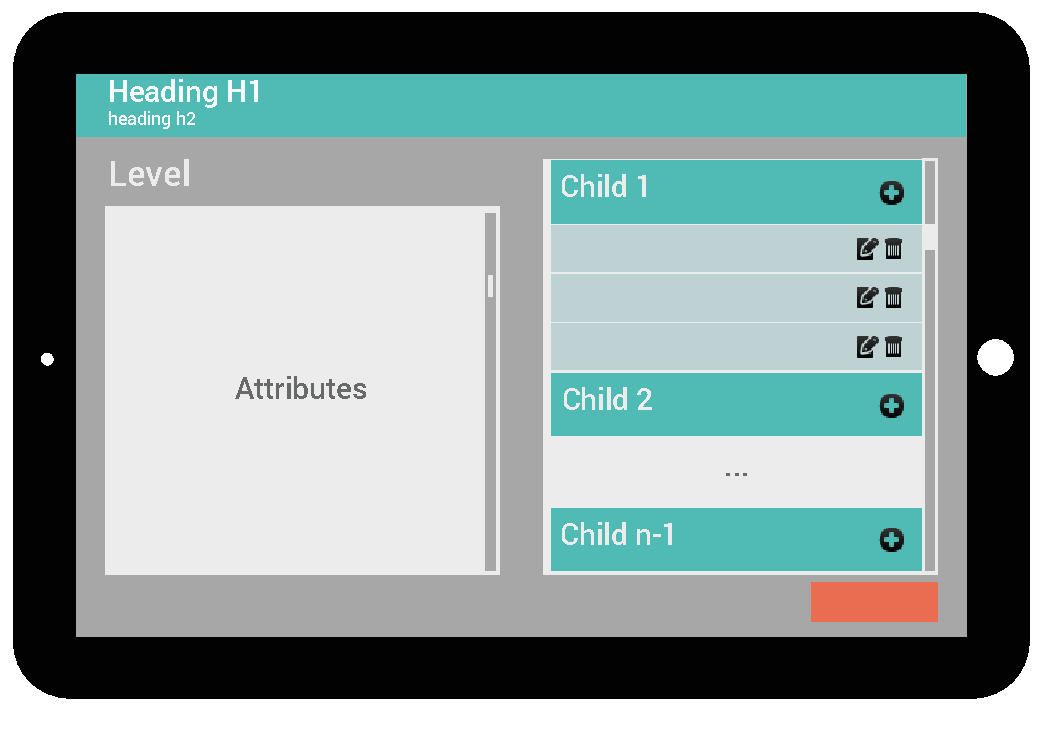
\includegraphics[scale=0.6]{./imgs/esquemas/layoutAttributesChildren.pdf}
\caption{Distribución de la interfaz de usuario con atributos e hijos}
\label{fig:layoutAC}
\end{figure}

\begin{figure}[ht]
\centering
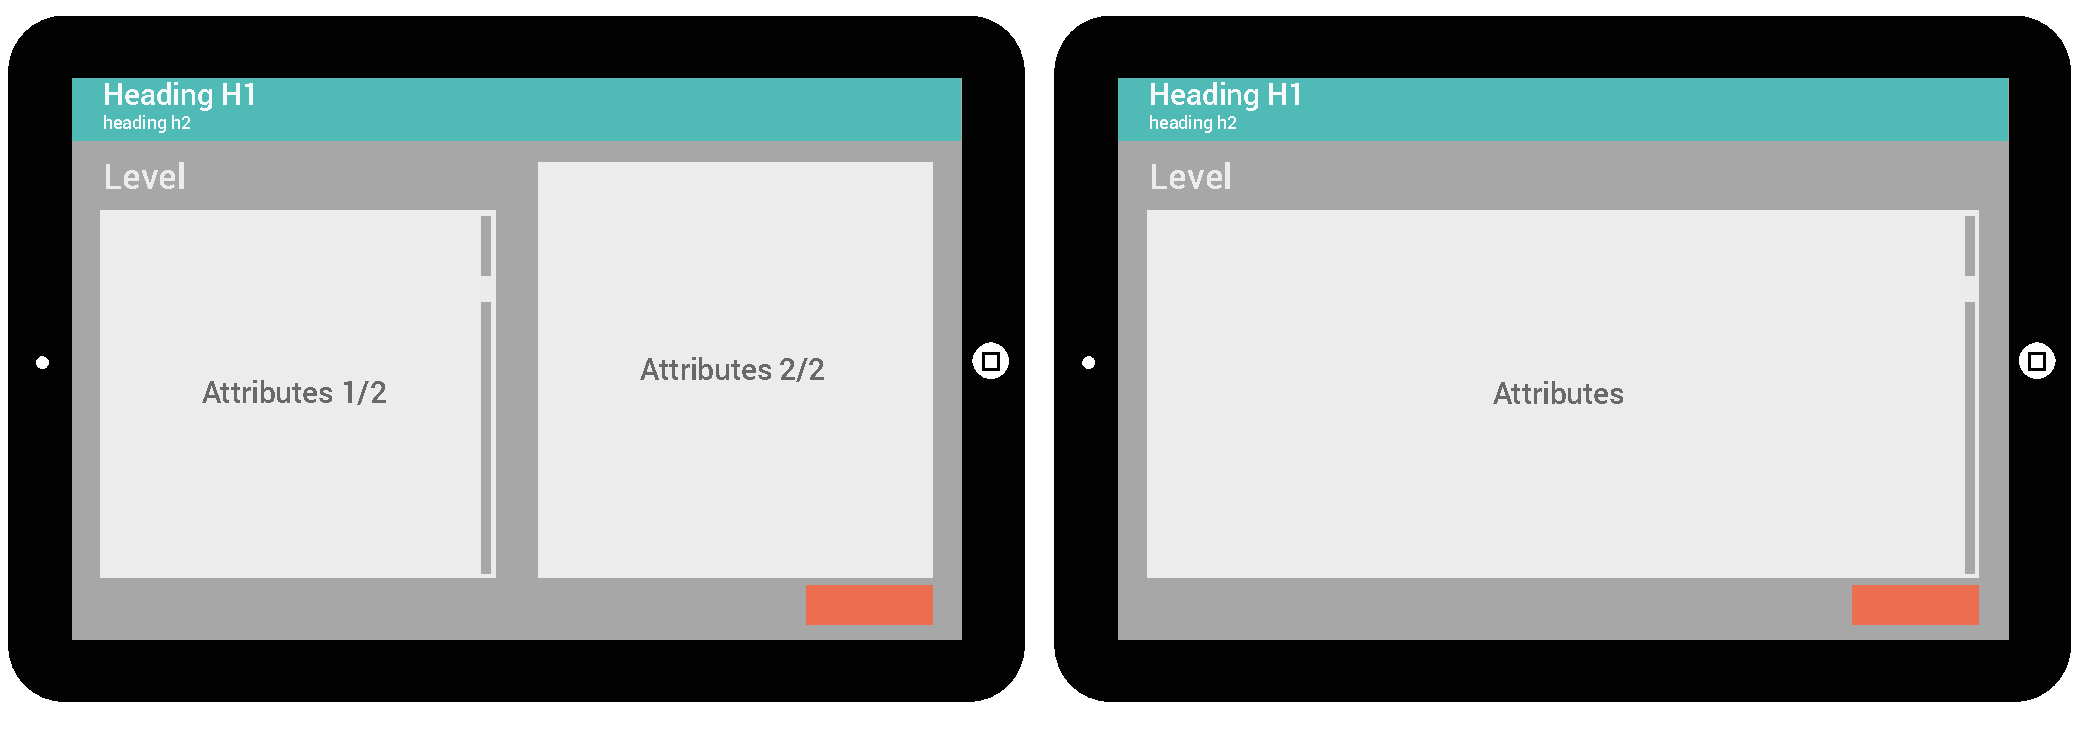
\includegraphics[scale=0.45]{./imgs/esquemas/layoutAttributes.pdf}
\caption{Distribución de la interfaz de usuario con atributos}
\label{fig:layoutA}
\end{figure}

\begin{figure}[ht]
\centering
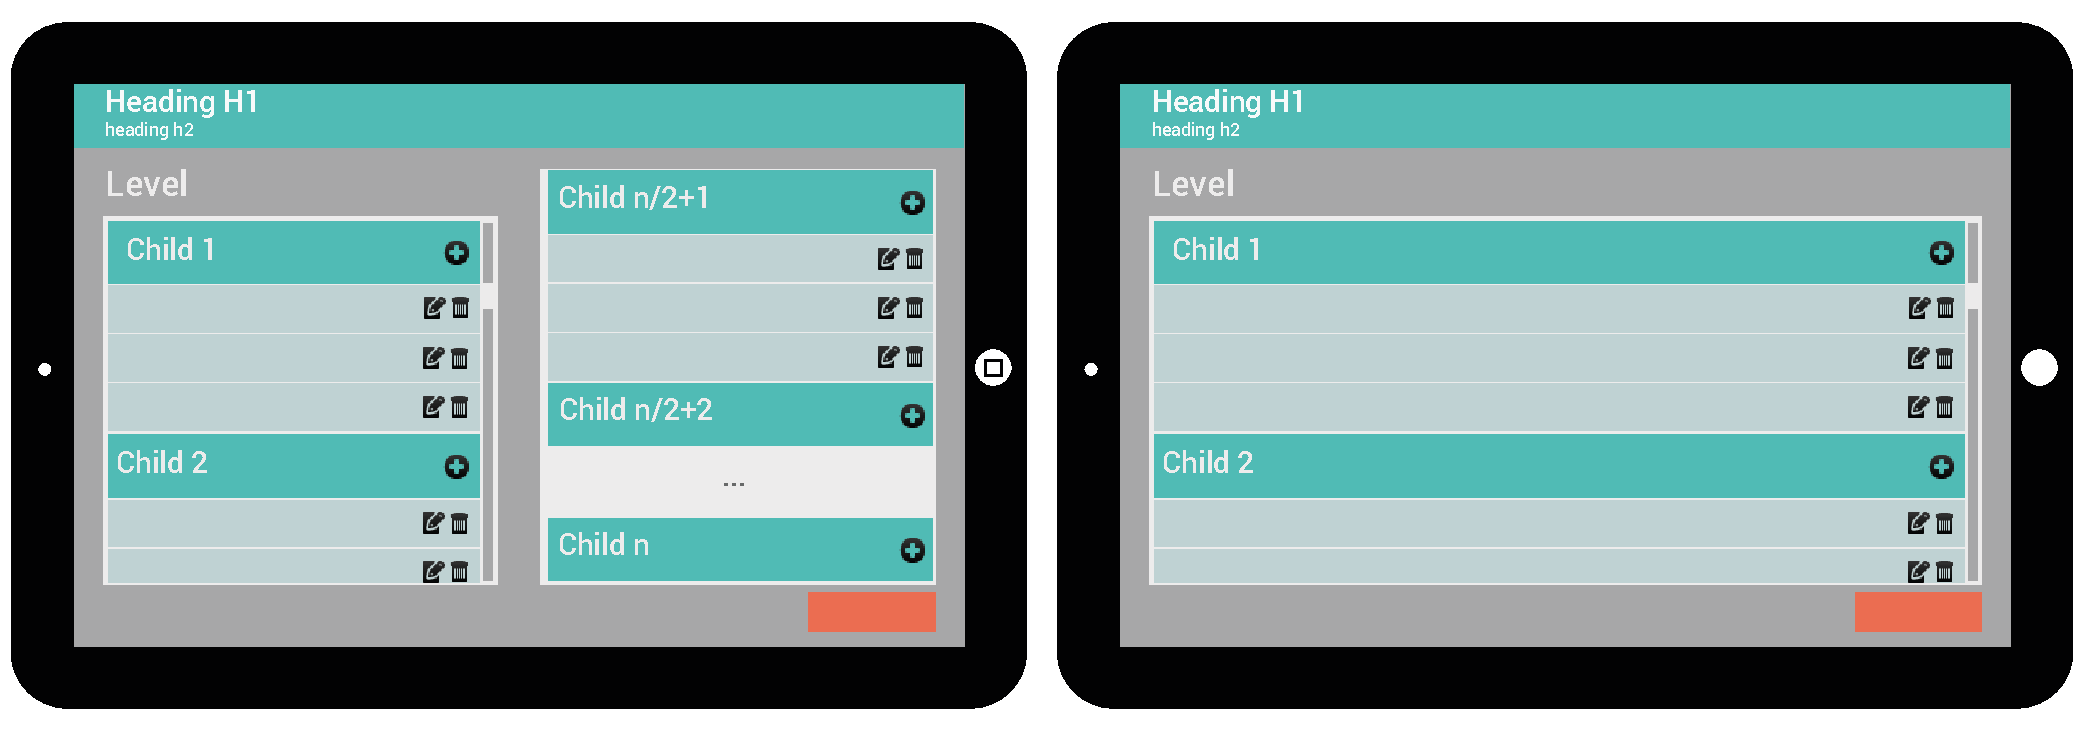
\includegraphics[scale=0.45]{./imgs/esquemas/layoutChildren.pdf}
\caption{Distribución de la interfaz de usuario con hijos}
\label{fig:layoutC}
\end{figure}

Diseñamos estas plantillas empleando el lenguaje de definición de plantillas de Jinja. Creamos una plantilla general (\emph{main.xml}), con los bloques de la interfaz de usuario que no varían (franja superior e inferior, segmento central, \ldots). Del mismo modo crearemos dos plantillas más, que extenderán el comportamiento de la plantilla general para codificar la interfaz de pantalla con una columna (\emph{one\_column.xml}) o con dos columnas (\emph{two\_columns.xml}).\par
El resto de los elementos de la interfaz de usuario (botones, campos de validación, campos de texto, \ldots) se diseñarán también utilizando Jinja. Todas estas plantillas son elementos modulares que se integrarán en la interfaz de usuario.\medskip\par

El programa generador de código se encarga de recorrer en anchura el árbol con el informe DICOM-SR y para cada nivel generar el fichero XML con la interfaz que le corresponda completando las plantillas Jinja con los datos concretos de este nivel.\par
Este fichero se almacenará en la ruta indicada por el usuario en la configuración. \par


\subsubsection{Generador de las cadenas de texto}\label{vista:strings}
Los elementos de la interfaz de usuario que acabamos de crear no muestran ningún texto. En el campo destinado a almacenar una cadena de texto hemos escrito el identificador de un recurso. En este apartado crearemos los ficheros con las cadenas de texto que se mostrarán en el informe.\par
De nuevo tenemos una serie de plantillas Jinja para definir los recursos de texto que tendrá disponibles la aplicación Android.\par
Rellenar estas plantillas es mucho más sencillo que en el apartado anterior porque no necesitamos información de la estructura del árbol, únicamente necesitamos un conjunto (sin repetidos) de todos los \emph{CONCEPT\_MEANING} que aparecen en el informe DICOM-SR. Extraemos este conjunto del árbol y rellenamos las plantillas. \medskip\par
La única complicación con la que debemos lidiar es la de identificar correctamente en que idioma está escrito el significado (\emph{CONCEPT\_MEANING}) de una etiqueta del informe DICOM-SR.\par 
Como en el propio informe no aparece la codificación del idioma,el usuario puede introducir el código en la configuración siguiendo el estándar ISO 3166-1-alpha-2. Este es el estándar que se utiliza en Android y consiste en 2 letras que identifican el idioma, un guión bajo ``\_'' y 2 letras más que identifican el país.\par 
Si el usuario no establece el idioma, el sistema asume que el texto está escrito en inglés si el informe no está internacionalizado y si está internacionalizado le adjudica el inglés al texto dentro de la etiqueta   \emph{CONCEPT\_MEANING2} y castellano para la etiqueta  \emph{CONCEPT\_MEANING}.

\subsection{Generador del controlador}

El último elemento que nos falta generar para completar la aplicación Android es el controlador. \par
En Android la visualización de la interfaz de usuario y la actualización del modelo de datos la realizan las actividades (\emph{Activity}). Una actividad es un componente de una aplicación Android que muestra una pantalla con la que el usuario puede interacturar. Cada actividad es responsable de cargar la interfaz de usuario definida mediante ficheros XML, crear los métodos que escuchen los eventos creados por la interacción con el usuario, interactuar con el modelo y por supuesto gestionar el ciclo de vida de la propia actividad.\medskip\par

%\subsubsection{Generador de las actividades}
% Caso general
El caso general para generar las actividades es análogo al descrito en los apartados \ref{sec:generacion_modelo} y \ref{vista:ui}. En este caso la información de la jerarquía del informe estructurado vuelve a ser relevante, por lo tanto recorreremos el árbol en anchura generando una clase que extiende el funcionamiento de la clase \emph{Activity}.\par
Al igual que en los casos anteriores hemos diseñado un conjunto de plantillas Jinja2 para modelar estas clases, y estas plantillas las completamos con la interfaz de usuario y los controladores correspondientes a los elementos del contenedor DICOM-SR.\medskip\par 

% Controladores para expandable listview
Para que las listas desplegables se comporten de manera adecuada a la funcionalidad que espera el usuario, deberemos crear adaptadores que extiendan el comportamiento básico de estas listas.\par
De nuevo, tendremos una plantilla Jinja2 para que los contenedores que precisen de listas desplegables las instancien.\medskip\par

% Manifest
Lo último que nos queda generar es el fichero \emph{AndroidManifest.txt}. Toda aplicación Android debe tener este fichero en el directorio raíz donde se encuentra el código.\par
Este fichero recoge toda la información fundamental de la aplicación al sistema. En este fichero debe figurar los siguientes elementos:
\begin{itemize}
\item El nombre del paquete de Java de la aplicación.
\item Los componentes de la aplicación Androdid: actividades, indicando cual es la actividad de inicio; servicios; proveedores de contenido; \ldots
\item Los permisos que necesita la aplicación para ejecutarse. 
\item La API mínima de Android que necesita la aplicación para ejecutarse. 
\end{itemize}
Definimos una plantilla Jinja2 con los elementos del manifiesto Android que instanciamos con los datos de la aplicación Android que hemos generado.\bigskip \par

Todos estos ficheros que hemos ido generando se integran dentro de la aplicación Android esqueleto componiendo una aplicación Android específica para el informe estructurado DICOM-SR de entrada.\par
Hemos conseguido una aplicación Android funcional a partir de un informe estructurado DICOM-SR.
%\section{Generador de la plantilla de resultados}


\chapter{Verificación: un caso práctico}
\section{Informe DICOM-SR}
\section{Generación automática de una aplicación Android}
\section{Aplicación Android para el informe de entrada}\label{sec:appfinal}

\chapter{Conclusiones}

\chapter{Futuras mejoras}

%\printbibliography
\bibliographystyle{unsrtnat}
\bibliography{bibliografia}

\appendix
\chapter{Informe DICOM-SR}\label{dicom-sr}
\lstset{escapechar=@,style=dicom}
\renewcommand*\lstlistingname{Fichero}

\begin{lstlisting}[label=dicom-report,caption=Informe estructurado de una exploración de mama]

<?xml version="1.0" encoding="ISO-8859-1"?>

<!-- DICOM HEADER -->

<DICOM_SR Description="Exploration of breast" IDOntology="4">
  <CONTAINER>
    <CONCEPT_NAME>
      <CODE_VALUE>172117008</CODE_VALUE>
      <CODE_SCHEMA>SNOMED-CT</CODE_SCHEMA>
      <CODE_MEANING>Exploration of Breast</CODE_MEANING>
    </CONCEPT_NAME>
    <CHILDS>
      <DATE>
        <CONCEPT_NAME>
          <CODE_VALUE>399651003</CODE_VALUE>
          <CODE_SCHEMA>SNOMED-CT</CODE_SCHEMA>
          <CODE_MEANING>Date of Report</CODE_MEANING>
        </CONCEPT_NAME>
        <VALUE> 28-07-2007 </VALUE>
      </DATE>
      <NUM>
        <CONCEPT_NAME>
          <CODE_VALUE>118522005</CODE_VALUE>
          <CODE_SCHEMA>SNOMED-CT</CODE_SCHEMA>
          <CODE_MEANING>Identifier</CODE_MEANING>
        </CONCEPT_NAME>
        <VALUE> 1234ABC </VALUE>
      </NUM>
      <NUM>
        <CONCEPT_NAME>
          <CODE_VALUE>RID13159</CODE_VALUE>
          <CODE_SCHEMA>RADLEX</CODE_SCHEMA>
          <CODE_MEANING>Patient Identifier</CODE_MEANING>
        </CONCEPT_NAME>
        <VALUE> 12345678X </VALUE>
      </NUM>

      <!-- RIGHT FEMALE BREAST -->
      <CONTAINER>
        <CONCEPT_NAME>
         <CODE_VALUE>RID29896</CODE_VALUE>
         <CODE_SCHEMA>RADLEX</CODE_SCHEMA>
         <CODE_MEANING>Right Female Breast</CODE_MEANING>
        </CONCEPT_NAME>

        <!-- RIGHT FEMALE BREAST INJURIES -->
        <CHILDS>
          <CONTAINER>
            <CONCEPT_NAME>
              <CODE_VALUE>RID3874</CODE_VALUE>
              <CODE_SCHEMA>RADLEX</CODE_SCHEMA>
              <CODE_MEANING>Mass</CODE_MEANING>
            </CONCEPT_NAME>
            <CHILDS>
              <TEXT>
                <CONCEPT_NAME>
                  <CODE_VALUE>118522005</CODE_VALUE>
                  <CODE_SCHEMA>SNOMED-CT</CODE_SCHEMA>
                  <CODE_MEANING>Identifier</CODE_MEANING>
                </CONCEPT_NAME>
                <VALUE> M001 </VALUE>
              </TEXT>
              <NUM>
                <CONCEPT_NAME>
                  <CODE_VALUE>RID29929</CODE_VALUE>
                  <CODE_SCHEMA>RADLEX</CODE_SCHEMA>
                  <CODE_MEANING>Upper Outer Quadrant of Right Female Breast</CODE_MEANING>
                </CONCEPT_NAME>
                <VALUE> TRUE </VALUE>
              </NUM>
              <NUM>
                <CONCEPT_NAME>
                  <CODE_VALUE>RID29935</CODE_VALUE>
                  <CODE_SCHEMA>RADLEX</CODE_SCHEMA>
                  <CODE_MEANING>Lower Outer Quadrant of Right Female Breast</CODE_MEANING>
                </CONCEPT_NAME>
                <VALUE> TRUE </VALUE>
              </NUM>
              <NUM>
                <CONCEPT_NAME>
                  <CODE_VALUE>RID29934</CODE_VALUE>
                  <CODE_SCHEMA>RADLEX</CODE_SCHEMA>
                  <CODE_MEANING>Lower Outer Quadrant of Breast</CODE_MEANING>
                </CONCEPT_NAME>
                <VALUE> FALSE </VALUE>
              </NUM>
              <NUM>
                <CONCEPT_NAME>
                  <CODE_VALUE>RID29932</CODE_VALUE>
                  <CODE_SCHEMA>RADLEX</CODE_SCHEMA>
                  <CODE_MEANING>Upper Inner Quadrant of Right Female Breast</CODE_MEANING>
                </CONCEPT_NAME>
                <VALUE> FALSE </VALUE>
              </NUM>
              <NUM>
                <CONCEPT_NAME>
                  <CODE_VALUE>RID29938</CODE_VALUE>
                  <CODE_SCHEMA>RADLEX</CODE_SCHEMA>
                  <CODE_MEANING>Lower Inner Quadrant of Right Female Breast</CODE_MEANING>
                </CONCEPT_NAME>
                <VALUE> FALSE </VALUE>
              </NUM>
              <NUM>
                <CONCEPT_NAME>
                  <CODE_VALUE>RID29947</CODE_VALUE>
                  <CODE_SCHEMA>RADLEX</CODE_SCHEMA>
                  <CODE_MEANING>Lateral Region of Right Female Breast</CODE_MEANING>
                </CONCEPT_NAME>
                <VALUE> FALSE </VALUE>
              </NUM>
              <NUM>
                <CONCEPT_NAME>
                  <CODE_VALUE>RID29941</CODE_VALUE>
                  <CODE_SCHEMA>RADLEX</CODE_SCHEMA>
                  <CODE_MEANING>Superior Region of Right Female Breast</CODE_MEANING>
                </CONCEPT_NAME>
                <VALUE> TRUE </VALUE>
              </NUM>
              <NUM>
                <CONCEPT_NAME>
                  <CODE_VALUE>RID29953</CODE_VALUE>
                  <CODE_SCHEMA>RADLEX</CODE_SCHEMA>
                  <CODE_MEANING>Subareolar Region of  Right Female Breast</CODE_MEANING>
                </CONCEPT_NAME>
                <VALUE> FALSE </VALUE>
              </NUM>
              <NUM>
                <CONCEPT_NAME>
                  <CODE_VALUE>RID29944</CODE_VALUE>
                  <CODE_SCHEMA>RADLEX</CODE_SCHEMA>
                  <CODE_MEANING>Medial Region of Right Breast</CODE_MEANING>
                </CONCEPT_NAME>
                <VALUE> FALSE </VALUE>
              </NUM>
              <NUM>	
                <CONCEPT_NAME>
                  <CODE_VALUE>RID29950</CODE_VALUE>
                  <CODE_SCHEMA>RADLEX</CODE_SCHEMA>
                  <CODE_MEANING>Central Region of Right Breast</CODE_MEANING>
                </CONCEPT_NAME>
                <VALUE> FALSE </VALUE>
              </NUM>
              <NUM>
                <CONCEPT_NAME>
                  <CODE_VALUE>RID29907</CODE_VALUE>
                  <CODE_SCHEMA>RADLEX</CODE_SCHEMA>
                  <CODE_MEANING>Nipple of Right Female Breast</CODE_MEANING>
                </CONCEPT_NAME>
                <VALUE> FALSE </VALUE>
              </NUM>
              <NUM>
                <CONCEPT_NAME>
                  <CODE_VALUE>RID29918</CODE_VALUE>
                  <CODE_SCHEMA>RADLEX</CODE_SCHEMA>
                  <CODE_MEANING>Areola of Right Female Breast</CODE_MEANING>
                </CONCEPT_NAME>
                <VALUE> FALSE </VALUE>
              </NUM>
              <NUM>
                <CONCEPT_NAME>
                  <CODE_VALUE>TRMM0001</CODE_VALUE>
                  <CODE_SCHEMA>TRENCADIS_MAMO</CODE_SCHEMA>
                  <CODE_MEANING>Axillary Tail of Right Female Breast</CODE_MEANING>
                </CONCEPT_NAME>
                <VALUE> FALSE </VALUE>
              </NUM>
              <NUM>
                <CONCEPT_NAME>
                  <CODE_VALUE>TRMM0003</CODE_VALUE>
                  <CODE_SCHEMA>TRENCADIS_MAMO</CODE_SCHEMA>
                  <CODE_MEANING>Axillary Region of Right Female Breast</CODE_MEANING>
                </CONCEPT_NAME>
                <VALUE> FALSE </VALUE>
              </NUM>
              <NUM>
                <CONCEPT_NAME>
                  <CODE_VALUE>TRMM0005</CODE_VALUE>
                  <CODE_SCHEMA>TRENCADIS_MAMO</CODE_SCHEMA>
                  <CODE_MEANING>Inframammary Sulcus of Right Female Breast</CODE_MEANING>
                </CONCEPT_NAME>
              </NUM>
              <NUM>
                <CONCEPT_NAME>
                  <CODE_VALUE>TRMM0007</CODE_VALUE>
                  <CODE_SCHEMA>TRENCADIS_MAMO</CODE_SCHEMA>
                  <CODE_MEANING>Intermammary Sulcus of Right Female Breast</CODE_MEANING>
                </CONCEPT_NAME>
              </NUM>
            </CHILDS>
      </CONTAINER>

      <!-- LEFT FEMALE BREAST -->
      <CONTAINER>
        <CONCEPT_NAME>
         <CODE_VALUE>RID29897</CODE_VALUE>
         <CODE_SCHEMA>RADLEX</CODE_SCHEMA>
         <CODE_MEANING>Left Female Breast</CODE_MEANING>
        </CONCEPT_NAME>

        <!-- LEFT FEMALE BREAST INJURIES -->
        <CHILDS>
          <CONTAINER>
            <CONCEPT_NAME>
              <CODE_VALUE>RID34265</CODE_VALUE>
              <CODE_SCHEMA>RADLEX</CODE_SCHEMA>
              <CODE_MEANING>Asymmetry</CODE_MEANING>
            </CONCEPT_NAME>
            <CHILDS>
              <TEXT>
                <CONCEPT_NAME>
                  <CODE_VALUE>118522005</CODE_VALUE>
                  <CODE_SCHEMA>SNOMED-CT</CODE_SCHEMA>
                  <CODE_MEANING>Identifier</CODE_MEANING>
                </CONCEPT_NAME>
                <VALUE> A001 </VALUE>
              </TEXT>
              <NUM>
                <CONCEPT_NAME>
                  <CODE_VALUE>RID29930</CODE_VALUE>
                  <CODE_SCHEMA>RADLEX</CODE_SCHEMA>
                  <CODE_MEANING>Upper Outer Quadrant of Left Female Breast</CODE_MEANING>
                </CONCEPT_NAME>
                <VALUE> FALSE </VALUE>
              </NUM>
              <NUM>
                <CONCEPT_NAME>
                  <CODE_VALUE>RID29936</CODE_VALUE>
                  <CODE_SCHEMA>RADLEX</CODE_SCHEMA>
                  <CODE_MEANING>Lower Outer Quadrant of Left Female Breast</CODE_MEANING>
                <VALUE> FALSE </VALUE>
              </NUM>
              <NUM>
                <CONCEPT_NAME>
                  <CODE_VALUE>RID29933</CODE_VALUE>
                  <CODE_SCHEMA>RADLEX</CODE_SCHEMA>
                  <CODE_MEANING>Upper Inner Quadrant of Left Female Breast</CODE_MEANING>
                </CONCEPT_NAME>
                <VALUE> FALSE </VALUE>
              </NUM>
              <NUM>
                <CONCEPT_NAME>
                  <CODE_VALUE>RID29939</CODE_VALUE>
                  <CODE_SCHEMA>RADLEX</CODE_SCHEMA>
                  <CODE_MEANING>Lower Inner Quadrant of Left Female Breast</CODE_MEANING>
                </CONCEPT_NAME>
                <VALUE> FALSE </VALUE>
              </NUM>
              <NUM>
                <CONCEPT_NAME>
                  <CODE_VALUE>RID29948</CODE_VALUE>
                  <CODE_SCHEMA>RADLEX</CODE_SCHEMA>
                  <CODE_MEANING>Lateral Region of Left Breast</CODE_MEANING>
                </CONCEPT_NAME>
                <VALUE> TRUE </VALUE>
              </NUM>
              <NUM>
                <CONCEPT_NAME>
                  <CODE_VALUE>RID29942</CODE_VALUE>
                  <CODE_SCHEMA>RADLEX</CODE_SCHEMA>
                  <CODE_MEANING>Superior Region of Left Breast</CODE_MEANING>
                </CONCEPT_NAME>
                <VALUE> TRUE </VALUE>
              </NUM>
              <NUM>
                <CONCEPT_NAME>
                  <CODE_VALUE>RID29954</CODE_VALUE>
                  <CODE_SCHEMA>RADLEX</CODE_SCHEMA>
                  <CODE_MEANING>Subareolar Region of Left Breast</CODE_MEANING>
                </CONCEPT_NAME>
                <VALUE> FALSE </VALUE>
              </NUM>
              <NUM>
                <CONCEPT_NAME>
                  <CODE_VALUE>RID29945</CODE_VALUE>
                  <CODE_SCHEMA>RADLEX</CODE_SCHEMA>
                  <CODE_MEANING>Medial Region of Left Breast</CODE_MEANING>
                </CONCEPT_NAME>
                <VALUE> FALSE </VALUE>
              </NUM>
              <NUM>
                <CONCEPT_NAME>
                  <CODE_VALUE>RID29951</CODE_VALUE>
                  <CODE_SCHEMA>RADLEX</CODE_SCHEMA>
                  <CODE_MEANING>Central Region of Left Breast</CODE_MEANING>
                </CONCEPT_NAME>
                <VALUE> FALSE </VALUE>
              </NUM>
              <NUM>
                <CONCEPT_NAME>
                  <CODE_VALUE>RID29908</CODE_VALUE>
                  <CODE_SCHEMA>RADLEX</CODE_SCHEMA>
                  <CODE_MEANING>Nipple of Left Female Breast</CODE_MEANING>
                </CONCEPT_NAME>
                <VALUE> FALSE </VALUE>
              </NUM>
              <NUM>
                <CONCEPT_NAME>
                  <CODE_VALUE>RID29919</CODE_VALUE>
                  <CODE_SCHEMA>RADLEX</CODE_SCHEMA>
                  <CODE_MEANING>Areola of Left Female Breast</CODE_MEANING>
                </CONCEPT_NAME>
                <VALUE> FALSE </VALUE>
              </NUM>
              <NUM>
                <CONCEPT_NAME>
                  <CODE_VALUE>TRMM0002</CODE_VALUE>
                  <CODE_SCHEMA>TRENCADIS_MAMO</CODE_SCHEMA>
                  <CODE_MEANING>Axillary Tail of Left Female Breast</CODE_MEANING>
                </CONCEPT_NAME>
                <VALUE> FALSE </VALUE>
              </NUM>
              <NUM>
              <CONCEPT_NAME>
                <CODE_VALUE>TRMM0004</CODE_VALUE>
                <CODE_SCHEMA>TRENCADIS_MAMO</CODE_SCHEMA>
                  <CODE_MEANING>Axillary Region of Left Female Breast</CODE_MEANING>
                </CONCEPT_NAME>
                <VALUE> FALSE </VALUE>
              </NUM>
              <NUM>
                <CONCEPT_NAME>
                  <CODE_VALUE>TRMM0006</CODE_VALUE>
                  <CODE_SCHEMA>TRENCADIS_MAMO</CODE_SCHEMA>
                  <CODE_MEANING>Inframammary Sulcus  of Left Female Breast</CODE_MEANING>
                </CONCEPT_NAME>
                <VALUE> FALSE </VALUE>
              </NUM>
              <NUM>
                <CONCEPT_NAME>
                  <CODE_VALUE>TRMM0008</CODE_VALUE>
                  <CODE_SCHEMA>TRENCADIS_MAMO</CODE_SCHEMA>
                  <CODE_MEANING>Intermammary Sulcus  of Left Female Breast</CODE_MEANING>
                </CONCEPT_NAME>
                <VALUE> FALSE </VALUE>
              </NUM>
            </CHILDS>
          </CONTAINER>
          <CONTAINER>
            <CONCEPT_NAME>
              <CODE_VALUE>RID34265</CODE_VALUE>
              <CODE_SCHEMA>RADLEX</CODE_SCHEMA>
              <CODE_MEANING>Asymmetry</CODE_MEANING>
            </CONCEPT_NAME>
            <CHILDS>
              <TEXT>
                <CONCEPT_NAME>
                  <CODE_VALUE>118522005</CODE_VALUE>
                  <CODE_SCHEMA>SNOMED-CT</CODE_SCHEMA>
                  <CODE_MEANING>Identifier</CODE_MEANING>
                </CONCEPT_NAME>
                <VALUE> A002 </VALUE>
              </TEXT>
              <NUM>
                <CONCEPT_NAME>
                  <CODE_VALUE>RID29930</CODE_VALUE>
                  <CODE_SCHEMA>RADLEX</CODE_SCHEMA>
                  <CODE_MEANING>Upper Outer Quadrant of Left Female Breast</CODE_MEANING>
                </CONCEPT_NAME>
                <VALUE> FALSE </VALUE>
              </NUM>
              <NUM>
                <CONCEPT_NAME>
                  <CODE_VALUE>RID29936</CODE_VALUE>
                  <CODE_SCHEMA>RADLEX</CODE_SCHEMA>
                  <CODE_MEANING>Lower Outer Quadrant of Left Female Breast</CODE_MEANING>
                <VALUE> FALSE </VALUE>
              </NUM>
              <NUM>
                <CONCEPT_NAME>
                  <CODE_VALUE>RID29933</CODE_VALUE>
                  <CODE_SCHEMA>RADLEX</CODE_SCHEMA>
                  <CODE_MEANING>Upper Inner Quadrant of Left Female Breast</CODE_MEANING>
                </CONCEPT_NAME>
                <VALUE> FALSE </VALUE>
              </NUM>
              <NUM>
                <CONCEPT_NAME>
                  <CODE_VALUE>RID29939</CODE_VALUE>
                  <CODE_SCHEMA>RADLEX</CODE_SCHEMA>
                  <CODE_MEANING>Lower Inner Quadrant of Left Female Breast</CODE_MEANING>
                </CONCEPT_NAME>
                <VALUE> FALSE </VALUE>
              </NUM>
              <NUM>
                <CONCEPT_NAME>
                  <CODE_VALUE>RID29948</CODE_VALUE>
                  <CODE_SCHEMA>RADLEX</CODE_SCHEMA>
                  <CODE_MEANING>Lateral Region of Left Breast</CODE_MEANING>
                </CONCEPT_NAME>
                <VALUE> FALSE </VALUE>
              </NUM>
              <NUM>
                <CONCEPT_NAME>
                  <CODE_VALUE>RID29942</CODE_VALUE>
                  <CODE_SCHEMA>RADLEX</CODE_SCHEMA>
                  <CODE_MEANING>Superior Region of Left Breast</CODE_MEANING>
                </CONCEPT_NAME>
                <VALUE> FALSE </VALUE>
              </NUM>
              <NUM>
                <CONCEPT_NAME>
                  <CODE_VALUE>RID29954</CODE_VALUE>
                  <CODE_SCHEMA>RADLEX</CODE_SCHEMA>
                  <CODE_MEANING>Subareolar Region of Left Breast</CODE_MEANING>
                </CONCEPT_NAME>
                <VALUE> FALSE </VALUE>
              </NUM>
              <NUM>
                <CONCEPT_NAME>
                  <CODE_VALUE>RID29945</CODE_VALUE>
                  <CODE_SCHEMA>RADLEX</CODE_SCHEMA>
                  <CODE_MEANING>Medial Region of Left Breast</CODE_MEANING>
                </CONCEPT_NAME>
                <VALUE> FALSE </VALUE>
              </NUM>
              <NUM>
                <CONCEPT_NAME>
                  <CODE_VALUE>RID29951</CODE_VALUE>
                  <CODE_SCHEMA>RADLEX</CODE_SCHEMA>
                  <CODE_MEANING>Central Region of Left Breast</CODE_MEANING>
                </CONCEPT_NAME>
                <VALUE> FALSE </VALUE>
              </NUM>
              <NUM>
                <CONCEPT_NAME>
                  <CODE_VALUE>RID29908</CODE_VALUE>
                  <CODE_SCHEMA>RADLEX</CODE_SCHEMA>
                  <CODE_MEANING>Nipple of Left Female Breast</CODE_MEANING>
                </CONCEPT_NAME>
                <VALUE> FALSE </VALUE>
              </NUM>
              <NUM>
                <CONCEPT_NAME>
                  <CODE_VALUE>RID29919</CODE_VALUE>
                  <CODE_SCHEMA>RADLEX</CODE_SCHEMA>
                  <CODE_MEANING>Areola of Left Female Breast</CODE_MEANING>
                </CONCEPT_NAME>
                <VALUE> FALSE </VALUE>
              </NUM>
              <NUM>
                <CONCEPT_NAME>
                  <CODE_VALUE>TRMM0002</CODE_VALUE>
                  <CODE_SCHEMA>TRENCADIS_MAMO</CODE_SCHEMA>
                  <CODE_MEANING>Axillary Tail of Left Female Breast</CODE_MEANING>
                </CONCEPT_NAME>
                <VALUE> TRUE </VALUE>
              </NUM>
              <NUM>
              <CONCEPT_NAME>
                <CODE_VALUE>TRMM0004</CODE_VALUE>
                <CODE_SCHEMA>TRENCADIS_MAMO</CODE_SCHEMA>
                  <CODE_MEANING>Axillary Region of Left Female Breast</CODE_MEANING>
                </CONCEPT_NAME>
                <VALUE> FALSE </VALUE>
              </NUM>
              <NUM>
                <CONCEPT_NAME>
                  <CODE_VALUE>TRMM0006</CODE_VALUE>
                  <CODE_SCHEMA>TRENCADIS_MAMO</CODE_SCHEMA>
                  <CODE_MEANING>Inframammary Sulcus  of Left Female Breast</CODE_MEANING>
                </CONCEPT_NAME>
                <VALUE> FALSE </VALUE>
              </NUM>
              <NUM>
                <CONCEPT_NAME>
                  <CODE_VALUE>TRMM0008</CODE_VALUE>
                  <CODE_SCHEMA>TRENCADIS_MAMO</CODE_SCHEMA>
                  <CODE_MEANING>Intermammary Sulcus  of Left Female Breast</CODE_MEANING>
                </CONCEPT_NAME>
                <VALUE> FALSE </VALUE>
              </NUM>
            </CHILDS>
          </CONTAINER>
        </CHILDS>
      </CONTAINER>
    </CHILDS>
  </CONTAINER>
<DICOM_SR>

\end{lstlisting}


\chapter{Plantilla de un informe DICOM-SR}\label{dicom-sr-template}
\lstset{escapechar=@,style=dicom}
\renewcommand*\lstlistingname{Fichero}

\begin{lstlisting}[label=dicom-template,caption=Plantilla de un informe estructurado de una exploración de mama]

<?xml version="1.0" encoding="ISO-8859-1"?>

<!-- DICOM HEADER -->

<DICOM_SR Description="Exploration of breast" IDOntology="4">
  <CONTAINER>
    <CONCEPT_NAME>
      <CODE_VALUE>172117008</CODE_VALUE>
      <CODE_SCHEMA>SNOMED-CT</CODE_SCHEMA>
      <CODE_MEANING>Exploration of Breast</CODE_MEANING>
    </CONCEPT_NAME>
    <PROPERTIES>
      <CARDINALITY max="1" min="1"/>
      <CONDITION_TYPE type="M"/>
      <EXPRESION_CONDITION xquery=""/>
    </PROPERTIES>
    <CHILDS>
      <DATE>
        <CONCEPT_NAME>
          <CODE_VALUE>399651003</CODE_VALUE>
          <CODE_SCHEMA>SNOMED-CT</CODE_SCHEMA>
          <CODE_MEANING>Date of Report</CODE_MEANING>
        </CONCEPT_NAME>
        <PROPERTIES>
          <CARDINALITY max="1" min="1"/>
          <CONDITION_TYPE type="M"/>
          <EXPRESION_CONDITION xquery=""/>
          <DEFAULT_VALUE value=""/>
        </PROPERTIES>
      </DATE>
      <NUM>
        <CONCEPT_NAME>
          <CODE_VALUE>118522005</CODE_VALUE>
          <CODE_SCHEMA>SNOMED-CT</CODE_SCHEMA>
          <CODE_MEANING>Identifier</CODE_MEANING>
        </CONCEPT_NAME>
        <PROPERTIES>
          <CARDINALITY max="1" min="1"/>
          <CONDITION_TYPE type="M"/>
          <EXPRESION_CONDITION xquery=""/>
          <DEFAULT_VALUE value=""/>
        </PROPERTIES>
      </NUM>
      <NUM>
        <CONCEPT_NAME>
          <CODE_VALUE>RID13159</CODE_VALUE>
          <CODE_SCHEMA>RADLEX</CODE_SCHEMA>
          <CODE_MEANING>Patient Identifier</CODE_MEANING>
        </CONCEPT_NAME>
        <PROPERTIES>
          <CARDINALITY max="1" min="1"/>
          <CONDITION_TYPE type="M"/>
          <EXPRESION_CONDITION xquery=""/>
          <DEFAULT_VALUE value=""/>
        </PROPERTIES>
      </NUM>

      <!-- RIGHT FEMALE BREAST -->
      <CONTAINER>
        <CONCEPT_NAME>
         <CODE_VALUE>RID29896</CODE_VALUE>
         <CODE_SCHEMA>RADLEX</CODE_SCHEMA>
         <CODE_MEANING>Right Female Breast</CODE_MEANING>
        </CONCEPT_NAME>
        <PROPERTIES>
          <CARDINALITY max="1" min="1"/>
          <CONDITION_TYPE type="M"/>
          <EXPRESION_CONDITION xquery=""/>
          <DEFAULT_VALUE value=""/>
        </PROPERTIES>

        <!-- RIGHT FEMALE BREAST INJURIES -->
        <CHILDS>
          <CONTAINER>
            <CONCEPT_NAME>
              <CODE_VALUE>RID3874</CODE_VALUE>
              <CODE_SCHEMA>RADLEX</CODE_SCHEMA>
              <CODE_MEANING>Mass</CODE_MEANING>
            </CONCEPT_NAME>
            <PROPERTIES>
              <CARDINALITY max="-1" min="0"/>
              <CONDITION_TYPE type="U"/>
              <EXPRESION_CONDITION xquery=""/>
            </PROPERTIES>
            <CHILDS>
              <TEXT>
                <CONCEPT_NAME>
                  <CODE_VALUE>118522005</CODE_VALUE>
                  <CODE_SCHEMA>SNOMED-CT</CODE_SCHEMA>
                  <CODE_MEANING>Identifier</CODE_MEANING>
                </CONCEPT_NAME>
                <PROPERTIES>
                  <CARDINALITY max="1" min="1"/>
                  <CONDITION_TYPE type="M"/>
                  <EXPRESION_CONDITION xquery=""/>
                  <DEFAULT_VALUE value=""/>
                </PROPERTIES>
              </TEXT>
              <NUM>
                <CONCEPT_NAME>
                  <CODE_VALUE>RID29929</CODE_VALUE>
                  <CODE_SCHEMA>RADLEX</CODE_SCHEMA>
                  <CODE_MEANING>Upper Outer Quadrant of Right Female Breast</CODE_MEANING>
                </CONCEPT_NAME>
                <PROPERTIES>
                  <CARDINALITY max="1" min="1"/>
                  <CONDITION_TYPE type="M"/>
                  <EXPRESION_CONDITION xquery=""/>
                  <DEFAULT_VALUE value="0"/>
                  <UNIT_MEASUREMENT>
                    <CONCEPT_NAME>
                      <CODE_VALUE>000000001</CODE_VALUE>
                      <CODE_SCHEMA>UNIT_MEASUREMENT</CODE_SCHEMA>
                      <CODE_MEANING>Boolean Units</CODE_MEANING>
                    </CONCEPT_NAME>
                  </UNIT_MEASUREMENT>
                </PROPERTIES>
              </NUM>
              <NUM>
                <CONCEPT_NAME>
                  <CODE_VALUE>RID29935</CODE_VALUE>
                  <CODE_SCHEMA>RADLEX</CODE_SCHEMA>
                  <CODE_MEANING>Lower Outer Quadrant of Right Female Breast</CODE_MEANING>
                </CONCEPT_NAME>
                <VALUE> TRUE </VALUE>
              </NUM>
              <NUM>
                <CONCEPT_NAME>
                  <CODE_VALUE>RID29934</CODE_VALUE>
                  <CODE_SCHEMA>RADLEX</CODE_SCHEMA>
                  <CODE_MEANING>Lower Outer Quadrant of Breast</CODE_MEANING>
                </CONCEPT_NAME>
                <PROPERTIES>
                  <CARDINALITY max="1" min="1"/>
                  <CONDITION_TYPE type="M"/>
                  <EXPRESION_CONDITION xquery=""/>
                  <DEFAULT_VALUE value="0"/>
                  <UNIT_MEASUREMENT>
                    <CONCEPT_NAME>
                      <CODE_VALUE>000000001</CODE_VALUE>
                      <CODE_SCHEMA>UNIT_MEASUREMENT</CODE_SCHEMA>
                      <CODE_MEANING>Boolean Units</CODE_MEANING>
                    </CONCEPT_NAME>
                  </UNIT_MEASUREMENT>
                </PROPERTIES>
              </NUM>
              <NUM>
                <CONCEPT_NAME>
                  <CODE_VALUE>RID29932</CODE_VALUE>
                  <CODE_SCHEMA>RADLEX</CODE_SCHEMA>
                  <CODE_MEANING>Upper Inner Quadrant of Right Female Breast</CODE_MEANING>
                </CONCEPT_NAME>
                <PROPERTIES>
                  <CARDINALITY max="1" min="1"/>
                  <CONDITION_TYPE type="M"/>
                  <EXPRESION_CONDITION xquery=""/>
                  <DEFAULT_VALUE value="0"/>
                  <UNIT_MEASUREMENT>
                    <CONCEPT_NAME>
                      <CODE_VALUE>000000001</CODE_VALUE>
                      <CODE_SCHEMA>UNIT_MEASUREMENT</CODE_SCHEMA>
                      <CODE_MEANING>Boolean Units</CODE_MEANING>
                    </CONCEPT_NAME>
                  </UNIT_MEASUREMENT>
                </PROPERTIES>
              </NUM>
              <NUM>
                <CONCEPT_NAME>
                  <CODE_VALUE>RID29938</CODE_VALUE>
                  <CODE_SCHEMA>RADLEX</CODE_SCHEMA>
                  <CODE_MEANING>Lower Inner Quadrant of Right Female Breast</CODE_MEANING>
                </CONCEPT_NAME>
                <PROPERTIES>
                  <CARDINALITY max="1" min="1"/>
                  <CONDITION_TYPE type="M"/>
                  <EXPRESION_CONDITION xquery=""/>
                  <DEFAULT_VALUE value="0"/>
                  <UNIT_MEASUREMENT>
                    <CONCEPT_NAME>
                      <CODE_VALUE>000000001</CODE_VALUE>
                      <CODE_SCHEMA>UNIT_MEASUREMENT</CODE_SCHEMA>
                      <CODE_MEANING>Boolean Units</CODE_MEANING>
                    </CONCEPT_NAME>
                  </UNIT_MEASUREMENT>
                </PROPERTIES>
              </NUM>
              <NUM>
                <CONCEPT_NAME>
                  <CODE_VALUE>RID29947</CODE_VALUE>
                  <CODE_SCHEMA>RADLEX</CODE_SCHEMA>
                  <CODE_MEANING>Lateral Region of Right Female Breast</CODE_MEANING>
                </CONCEPT_NAME>
                <PROPERTIES>
                  <CARDINALITY max="1" min="1"/>
                  <CONDITION_TYPE type="M"/>
                  <EXPRESION_CONDITION xquery=""/>
                  <DEFAULT_VALUE value="0"/>
                  <UNIT_MEASUREMENT>
                    <CONCEPT_NAME>
                      <CODE_VALUE>000000001</CODE_VALUE>
                      <CODE_SCHEMA>UNIT_MEASUREMENT</CODE_SCHEMA>
                      <CODE_MEANING>Boolean Units</CODE_MEANING>
                    </CONCEPT_NAME>
                  </UNIT_MEASUREMENT>
                </PROPERTIES>
              </NUM>
              <NUM>
                <CONCEPT_NAME>
                  <CODE_VALUE>RID29941</CODE_VALUE>
                  <CODE_SCHEMA>RADLEX</CODE_SCHEMA>
                  <CODE_MEANING>Superior Region of Right Female Breast</CODE_MEANING>
                </CONCEPT_NAME>
                <VALUE> TRUE </VALUE>
              </NUM>
              <NUM>
                <CONCEPT_NAME>
                  <CODE_VALUE>RID29953</CODE_VALUE>
                  <CODE_SCHEMA>RADLEX</CODE_SCHEMA>
                  <CODE_MEANING>Subareolar Region of  Right Female Breast</CODE_MEANING>
                </CONCEPT_NAME>
                <PROPERTIES>
                  <CARDINALITY max="1" min="1"/>
                  <CONDITION_TYPE type="M"/>
                  <EXPRESION_CONDITION xquery=""/>
                  <DEFAULT_VALUE value="0"/>
                  <UNIT_MEASUREMENT>
                    <CONCEPT_NAME>
                      <CODE_VALUE>000000001</CODE_VALUE>
                      <CODE_SCHEMA>UNIT_MEASUREMENT</CODE_SCHEMA>
                      <CODE_MEANING>Boolean Units</CODE_MEANING>
                    </CONCEPT_NAME>
                  </UNIT_MEASUREMENT>
                </PROPERTIES>
              </NUM>
              <NUM>
                <CONCEPT_NAME>
                  <CODE_VALUE>RID29944</CODE_VALUE>
                  <CODE_SCHEMA>RADLEX</CODE_SCHEMA>
                  <CODE_MEANING>Medial Region of Right Breast</CODE_MEANING>
                </CONCEPT_NAME>
                <PROPERTIES>
                  <CARDINALITY max="1" min="1"/>
                  <CONDITION_TYPE type="M"/>
                  <EXPRESION_CONDITION xquery=""/>
                  <DEFAULT_VALUE value="0"/>
                  <UNIT_MEASUREMENT>
                    <CONCEPT_NAME>
                      <CODE_VALUE>000000001</CODE_VALUE>
                      <CODE_SCHEMA>UNIT_MEASUREMENT</CODE_SCHEMA>
                      <CODE_MEANING>Boolean Units</CODE_MEANING>
                    </CONCEPT_NAME>
                  </UNIT_MEASUREMENT>
                </PROPERTIES>
              </NUM>
              <NUM>	
                <CONCEPT_NAME>
                  <CODE_VALUE>RID29950</CODE_VALUE>
                  <CODE_SCHEMA>RADLEX</CODE_SCHEMA>
                  <CODE_MEANING>Central Region of Right Breast</CODE_MEANING>
                </CONCEPT_NAME>
                <PROPERTIES>
                  <CARDINALITY max="1" min="1"/>
                  <CONDITION_TYPE type="M"/>
                  <EXPRESION_CONDITION xquery=""/>
                  <DEFAULT_VALUE value="0"/>
                  <UNIT_MEASUREMENT>
                    <CONCEPT_NAME>
                      <CODE_VALUE>000000001</CODE_VALUE>
                      <CODE_SCHEMA>UNIT_MEASUREMENT</CODE_SCHEMA>
                      <CODE_MEANING>Boolean Units</CODE_MEANING>
                    </CONCEPT_NAME>
                  </UNIT_MEASUREMENT>
                </PROPERTIES>
              </NUM>
              <NUM>
                <CONCEPT_NAME>
                  <CODE_VALUE>RID29907</CODE_VALUE>
                  <CODE_SCHEMA>RADLEX</CODE_SCHEMA>
                  <CODE_MEANING>Nipple of Right Female Breast</CODE_MEANING>
                </CONCEPT_NAME>
                <PROPERTIES>
                  <CARDINALITY max="1" min="1"/>
                  <CONDITION_TYPE type="M"/>
                  <EXPRESION_CONDITION xquery=""/>
                  <DEFAULT_VALUE value="0"/>
                  <UNIT_MEASUREMENT>
                    <CONCEPT_NAME>
                      <CODE_VALUE>000000001</CODE_VALUE>
                      <CODE_SCHEMA>UNIT_MEASUREMENT</CODE_SCHEMA>
                      <CODE_MEANING>Boolean Units</CODE_MEANING>
                    </CONCEPT_NAME>
                  </UNIT_MEASUREMENT>
                </PROPERTIES>
              </NUM>
              <NUM>
                <CONCEPT_NAME>
                  <CODE_VALUE>RID29918</CODE_VALUE>
                  <CODE_SCHEMA>RADLEX</CODE_SCHEMA>
                  <CODE_MEANING>Areola of Right Female Breast</CODE_MEANING>
                </CONCEPT_NAME>
                <PROPERTIES>
                  <CARDINALITY max="1" min="1"/>
                  <CONDITION_TYPE type="M"/>
                  <EXPRESION_CONDITION xquery=""/>
                  <DEFAULT_VALUE value="0"/>
                  <UNIT_MEASUREMENT>
                    <CONCEPT_NAME>
                      <CODE_VALUE>000000001</CODE_VALUE>
                      <CODE_SCHEMA>UNIT_MEASUREMENT</CODE_SCHEMA>
                      <CODE_MEANING>Boolean Units</CODE_MEANING>
                    </CONCEPT_NAME>
                  </UNIT_MEASUREMENT>
                </PROPERTIES>
              </NUM>
              <NUM>
                <CONCEPT_NAME>
                  <CODE_VALUE>TRMM0001</CODE_VALUE>
                  <CODE_SCHEMA>TRENCADIS_MAMO</CODE_SCHEMA>
                  <CODE_MEANING>Axillary Tail of Right Female Breast</CODE_MEANING>
                </CONCEPT_NAME>
                <PROPERTIES>
                  <CARDINALITY max="1" min="1"/>
                  <CONDITION_TYPE type="M"/>
                  <EXPRESION_CONDITION xquery=""/>
                  <DEFAULT_VALUE value="0"/>
                  <UNIT_MEASUREMENT>
                    <CONCEPT_NAME>
                      <CODE_VALUE>000000001</CODE_VALUE>
                      <CODE_SCHEMA>UNIT_MEASUREMENT</CODE_SCHEMA>
                      <CODE_MEANING>Boolean Units</CODE_MEANING>
                    </CONCEPT_NAME>
                  </UNIT_MEASUREMENT>
                </PROPERTIES>
              </NUM>
              <NUM>
                <CONCEPT_NAME>
                  <CODE_VALUE>TRMM0003</CODE_VALUE>
                  <CODE_SCHEMA>TRENCADIS_MAMO</CODE_SCHEMA>
                  <CODE_MEANING>Axillary Region of Right Female Breast</CODE_MEANING>
                </CONCEPT_NAME>
                <PROPERTIES>
                  <CARDINALITY max="1" min="1"/>
                  <CONDITION_TYPE type="M"/>
                  <EXPRESION_CONDITION xquery=""/>
                  <DEFAULT_VALUE value="0"/>
                  <UNIT_MEASUREMENT>
                    <CONCEPT_NAME>
                      <CODE_VALUE>000000001</CODE_VALUE>
                      <CODE_SCHEMA>UNIT_MEASUREMENT</CODE_SCHEMA>
                      <CODE_MEANING>Boolean Units</CODE_MEANING>
                    </CONCEPT_NAME>
                  </UNIT_MEASUREMENT>
                </PROPERTIES>
              </NUM>
              <NUM>
                <CONCEPT_NAME>
                  <CODE_VALUE>TRMM0005</CODE_VALUE>
                  <CODE_SCHEMA>TRENCADIS_MAMO</CODE_SCHEMA>
                  <CODE_MEANING>Inframammary Sulcus of Right Female Breast</CODE_MEANING>
                </CONCEPT_NAME>
              </NUM>
              <NUM>
                <CONCEPT_NAME>
                  <CODE_VALUE>TRMM0007</CODE_VALUE>
                  <CODE_SCHEMA>TRENCADIS_MAMO</CODE_SCHEMA>
                  <CODE_MEANING>Intermammary Sulcus of Right Female Breast</CODE_MEANING>
                </CONCEPT_NAME>
              </NUM>
            </CHILDS>
      </CONTAINER>

      <!-- LEFT FEMALE BREAST -->
      <CONTAINER>
        <CONCEPT_NAME>
         <CODE_VALUE>RID29897</CODE_VALUE>
         <CODE_SCHEMA>RADLEX</CODE_SCHEMA>
         <CODE_MEANING>Left Female Breast</CODE_MEANING>
        </CONCEPT_NAME>

        <!-- LEFT FEMALE BREAST INJURIES -->
        <CHILDS>
          <CONTAINER>
            <CONCEPT_NAME>
              <CODE_VALUE>RID34265</CODE_VALUE>
              <CODE_SCHEMA>RADLEX</CODE_SCHEMA>
              <CODE_MEANING>Asymmetry</CODE_MEANING>
            </CONCEPT_NAME>
            <CHILDS>
              <TEXT>
                <CONCEPT_NAME>
                  <CODE_VALUE>118522005</CODE_VALUE>
                  <CODE_SCHEMA>SNOMED-CT</CODE_SCHEMA>
                  <CODE_MEANING>Identifier</CODE_MEANING>
                </CONCEPT_NAME>
                <VALUE> A001 </VALUE>
              </TEXT>
              <NUM>
                <CONCEPT_NAME>
                  <CODE_VALUE>RID29930</CODE_VALUE>
                  <CODE_SCHEMA>RADLEX</CODE_SCHEMA>
                  <CODE_MEANING>Upper Outer Quadrant of Left Female Breast</CODE_MEANING>
                </CONCEPT_NAME>
                <PROPERTIES>
                  <CARDINALITY max="1" min="1"/>
                  <CONDITION_TYPE type="M"/>
                  <EXPRESION_CONDITION xquery=""/>
                  <DEFAULT_VALUE value="0"/>
                  <UNIT_MEASUREMENT>
                    <CONCEPT_NAME>
                      <CODE_VALUE>000000001</CODE_VALUE>
                      <CODE_SCHEMA>UNIT_MEASUREMENT</CODE_SCHEMA>
                      <CODE_MEANING>Boolean Units</CODE_MEANING>
                    </CONCEPT_NAME>
                  </UNIT_MEASUREMENT>
                </PROPERTIES>
              </NUM>
              <NUM>
                <CONCEPT_NAME>
                  <CODE_VALUE>RID29936</CODE_VALUE>
                  <CODE_SCHEMA>RADLEX</CODE_SCHEMA>
                  <CODE_MEANING>Lower Outer Quadrant of Left Female Breast</CODE_MEANING>
                <PROPERTIES>
                  <CARDINALITY max="1" min="1"/>
                  <CONDITION_TYPE type="M"/>
                  <EXPRESION_CONDITION xquery=""/>
                  <DEFAULT_VALUE value="0"/>
                  <UNIT_MEASUREMENT>
                    <CONCEPT_NAME>
                      <CODE_VALUE>000000001</CODE_VALUE>
                      <CODE_SCHEMA>UNIT_MEASUREMENT</CODE_SCHEMA>
                      <CODE_MEANING>Boolean Units</CODE_MEANING>
                    </CONCEPT_NAME>
                  </UNIT_MEASUREMENT>
                </PROPERTIES>
              </NUM>
              <NUM>
                <CONCEPT_NAME>
                  <CODE_VALUE>RID29933</CODE_VALUE>
                  <CODE_SCHEMA>RADLEX</CODE_SCHEMA>
                  <CODE_MEANING>Upper Inner Quadrant of Left Female Breast</CODE_MEANING>
                </CONCEPT_NAME>
                <PROPERTIES>
                  <CARDINALITY max="1" min="1"/>
                  <CONDITION_TYPE type="M"/>
                  <EXPRESION_CONDITION xquery=""/>
                  <DEFAULT_VALUE value="0"/>
                  <UNIT_MEASUREMENT>
                    <CONCEPT_NAME>
                      <CODE_VALUE>000000001</CODE_VALUE>
                      <CODE_SCHEMA>UNIT_MEASUREMENT</CODE_SCHEMA>
                      <CODE_MEANING>Boolean Units</CODE_MEANING>
                    </CONCEPT_NAME>
                  </UNIT_MEASUREMENT>
                </PROPERTIES>
              </NUM>
              <NUM>
                <CONCEPT_NAME>
                  <CODE_VALUE>RID29939</CODE_VALUE>
                  <CODE_SCHEMA>RADLEX</CODE_SCHEMA>
                  <CODE_MEANING>Lower Inner Quadrant of Left Female Breast</CODE_MEANING>
                </CONCEPT_NAME>
                <PROPERTIES>
                  <CARDINALITY max="1" min="1"/>
                  <CONDITION_TYPE type="M"/>
                  <EXPRESION_CONDITION xquery=""/>
                  <DEFAULT_VALUE value="0"/>
                  <UNIT_MEASUREMENT>
                    <CONCEPT_NAME>
                      <CODE_VALUE>000000001</CODE_VALUE>
                      <CODE_SCHEMA>UNIT_MEASUREMENT</CODE_SCHEMA>
                      <CODE_MEANING>Boolean Units</CODE_MEANING>
                    </CONCEPT_NAME>
                  </UNIT_MEASUREMENT>
                </PROPERTIES>
              </NUM>
              <NUM>
                <CONCEPT_NAME>
                  <CODE_VALUE>RID29948</CODE_VALUE>
                  <CODE_SCHEMA>RADLEX</CODE_SCHEMA>
                  <CODE_MEANING>Lateral Region of Left Breast</CODE_MEANING>
                </CONCEPT_NAME>
                <VALUE> TRUE </VALUE>
              </NUM>
              <NUM>
                <CONCEPT_NAME>
                  <CODE_VALUE>RID29942</CODE_VALUE>
                  <CODE_SCHEMA>RADLEX</CODE_SCHEMA>
                  <CODE_MEANING>Superior Region of Left Breast</CODE_MEANING>
                </CONCEPT_NAME>
                <VALUE> TRUE </VALUE>
              </NUM>
              <NUM>
                <CONCEPT_NAME>
                  <CODE_VALUE>RID29954</CODE_VALUE>
                  <CODE_SCHEMA>RADLEX</CODE_SCHEMA>
                  <CODE_MEANING>Subareolar Region of Left Breast</CODE_MEANING>
                </CONCEPT_NAME>
                <PROPERTIES>
                  <CARDINALITY max="1" min="1"/>
                  <CONDITION_TYPE type="M"/>
                  <EXPRESION_CONDITION xquery=""/>
                  <DEFAULT_VALUE value="0"/>
                  <UNIT_MEASUREMENT>
                    <CONCEPT_NAME>
                      <CODE_VALUE>000000001</CODE_VALUE>
                      <CODE_SCHEMA>UNIT_MEASUREMENT</CODE_SCHEMA>
                      <CODE_MEANING>Boolean Units</CODE_MEANING>
                    </CONCEPT_NAME>
                  </UNIT_MEASUREMENT>
                </PROPERTIES>
              </NUM>
              <NUM>
                <CONCEPT_NAME>
                  <CODE_VALUE>RID29945</CODE_VALUE>
                  <CODE_SCHEMA>RADLEX</CODE_SCHEMA>
                  <CODE_MEANING>Medial Region of Left Breast</CODE_MEANING>
                </CONCEPT_NAME>
                <PROPERTIES>
                  <CARDINALITY max="1" min="1"/>
                  <CONDITION_TYPE type="M"/>
                  <EXPRESION_CONDITION xquery=""/>
                  <DEFAULT_VALUE value="0"/>
                  <UNIT_MEASUREMENT>
                    <CONCEPT_NAME>
                      <CODE_VALUE>000000001</CODE_VALUE>
                      <CODE_SCHEMA>UNIT_MEASUREMENT</CODE_SCHEMA>
                      <CODE_MEANING>Boolean Units</CODE_MEANING>
                    </CONCEPT_NAME>
                  </UNIT_MEASUREMENT>
                </PROPERTIES>
              </NUM>
              <NUM>
                <CONCEPT_NAME>
                  <CODE_VALUE>RID29951</CODE_VALUE>
                  <CODE_SCHEMA>RADLEX</CODE_SCHEMA>
                  <CODE_MEANING>Central Region of Left Breast</CODE_MEANING>
                </CONCEPT_NAME>
                <PROPERTIES>
                  <CARDINALITY max="1" min="1"/>
                  <CONDITION_TYPE type="M"/>
                  <EXPRESION_CONDITION xquery=""/>
                  <DEFAULT_VALUE value="0"/>
                  <UNIT_MEASUREMENT>
                    <CONCEPT_NAME>
                      <CODE_VALUE>000000001</CODE_VALUE>
                      <CODE_SCHEMA>UNIT_MEASUREMENT</CODE_SCHEMA>
                      <CODE_MEANING>Boolean Units</CODE_MEANING>
                    </CONCEPT_NAME>
                  </UNIT_MEASUREMENT>
                </PROPERTIES>
              </NUM>
              <NUM>
                <CONCEPT_NAME>
                  <CODE_VALUE>RID29908</CODE_VALUE>
                  <CODE_SCHEMA>RADLEX</CODE_SCHEMA>
                  <CODE_MEANING>Nipple of Left Female Breast</CODE_MEANING>
                </CONCEPT_NAME>
                <PROPERTIES>
                  <CARDINALITY max="1" min="1"/>
                  <CONDITION_TYPE type="M"/>
                  <EXPRESION_CONDITION xquery=""/>
                  <DEFAULT_VALUE value="0"/>
                  <UNIT_MEASUREMENT>
                    <CONCEPT_NAME>
                      <CODE_VALUE>000000001</CODE_VALUE>
                      <CODE_SCHEMA>UNIT_MEASUREMENT</CODE_SCHEMA>
                      <CODE_MEANING>Boolean Units</CODE_MEANING>
                    </CONCEPT_NAME>
                  </UNIT_MEASUREMENT>
                </PROPERTIES>
              </NUM>
              <NUM>
                <CONCEPT_NAME>
                  <CODE_VALUE>RID29919</CODE_VALUE>
                  <CODE_SCHEMA>RADLEX</CODE_SCHEMA>
                  <CODE_MEANING>Areola of Left Female Breast</CODE_MEANING>
                </CONCEPT_NAME>
                <PROPERTIES>
                  <CARDINALITY max="1" min="1"/>
                  <CONDITION_TYPE type="M"/>
                  <EXPRESION_CONDITION xquery=""/>
                  <DEFAULT_VALUE value="0"/>
                  <UNIT_MEASUREMENT>
                    <CONCEPT_NAME>
                      <CODE_VALUE>000000001</CODE_VALUE>
                      <CODE_SCHEMA>UNIT_MEASUREMENT</CODE_SCHEMA>
                      <CODE_MEANING>Boolean Units</CODE_MEANING>
                    </CONCEPT_NAME>
                  </UNIT_MEASUREMENT>
                </PROPERTIES>
              </NUM>
              <NUM>
                <CONCEPT_NAME>
                  <CODE_VALUE>TRMM0002</CODE_VALUE>
                  <CODE_SCHEMA>TRENCADIS_MAMO</CODE_SCHEMA>
                  <CODE_MEANING>Axillary Tail of Left Female Breast</CODE_MEANING>
                </CONCEPT_NAME>
                <PROPERTIES>
                  <CARDINALITY max="1" min="1"/>
                  <CONDITION_TYPE type="M"/>
                  <EXPRESION_CONDITION xquery=""/>
                  <DEFAULT_VALUE value="0"/>
                  <UNIT_MEASUREMENT>
                    <CONCEPT_NAME>
                      <CODE_VALUE>000000001</CODE_VALUE>
                      <CODE_SCHEMA>UNIT_MEASUREMENT</CODE_SCHEMA>
                      <CODE_MEANING>Boolean Units</CODE_MEANING>
                    </CONCEPT_NAME>
                  </UNIT_MEASUREMENT>
                </PROPERTIES>
              </NUM>
              <NUM>
              <CONCEPT_NAME>
                <CODE_VALUE>TRMM0004</CODE_VALUE>
                <CODE_SCHEMA>TRENCADIS_MAMO</CODE_SCHEMA>
                  <CODE_MEANING>Axillary Region of Left Female Breast</CODE_MEANING>
                </CONCEPT_NAME>
                <PROPERTIES>
                  <CARDINALITY max="1" min="1"/>
                  <CONDITION_TYPE type="M"/>
                  <EXPRESION_CONDITION xquery=""/>
                  <DEFAULT_VALUE value="0"/>
                  <UNIT_MEASUREMENT>
                    <CONCEPT_NAME>
                      <CODE_VALUE>000000001</CODE_VALUE>
                      <CODE_SCHEMA>UNIT_MEASUREMENT</CODE_SCHEMA>
                      <CODE_MEANING>Boolean Units</CODE_MEANING>
                    </CONCEPT_NAME>
                  </UNIT_MEASUREMENT>
                </PROPERTIES>
              </NUM>
              <NUM>
                <CONCEPT_NAME>
                  <CODE_VALUE>TRMM0006</CODE_VALUE>
                  <CODE_SCHEMA>TRENCADIS_MAMO</CODE_SCHEMA>
                  <CODE_MEANING>Inframammary Sulcus  of Left Female Breast</CODE_MEANING>
                </CONCEPT_NAME>
                <PROPERTIES>
                  <CARDINALITY max="1" min="1"/>
                  <CONDITION_TYPE type="M"/>
                  <EXPRESION_CONDITION xquery=""/>
                  <DEFAULT_VALUE value="0"/>
                  <UNIT_MEASUREMENT>
                    <CONCEPT_NAME>
                      <CODE_VALUE>000000001</CODE_VALUE>
                      <CODE_SCHEMA>UNIT_MEASUREMENT</CODE_SCHEMA>
                      <CODE_MEANING>Boolean Units</CODE_MEANING>
                    </CONCEPT_NAME>
                  </UNIT_MEASUREMENT>
                </PROPERTIES>
              </NUM>
              <NUM>
                <CONCEPT_NAME>
                  <CODE_VALUE>TRMM0008</CODE_VALUE>
                  <CODE_SCHEMA>TRENCADIS_MAMO</CODE_SCHEMA>
                  <CODE_MEANING>Intermammary Sulcus  of Left Female Breast</CODE_MEANING>
                </CONCEPT_NAME>
                <PROPERTIES>
                  <CARDINALITY max="1" min="1"/>
                  <CONDITION_TYPE type="M"/>
                  <EXPRESION_CONDITION xquery=""/>
                  <DEFAULT_VALUE value="0"/>
                  <UNIT_MEASUREMENT>
                    <CONCEPT_NAME>
                      <CODE_VALUE>000000001</CODE_VALUE>
                      <CODE_SCHEMA>UNIT_MEASUREMENT</CODE_SCHEMA>
                      <CODE_MEANING>Boolean Units</CODE_MEANING>
                    </CONCEPT_NAME>
                  </UNIT_MEASUREMENT>
                </PROPERTIES>
              </NUM>
            </CHILDS>
          </CONTAINER>
        </CHILDS>
      </CONTAINER>
    </CHILDS>
  </CONTAINER>
<DICOM_SR>

\end{lstlisting}



\end{document}